\chapter{Použité prostředky a~hardware}\label{kap:prostredky}
	\section{Interpolátor}
	
	Jednotku interpolátoru jsem se rozhodl postavit na STM32F4 Dicovery kitu. Tento vývojový kit je postaven na STM32F407VGT6 ARM mikrokontroléru\cite{discovery}. Kit obsahuje integrovaný debugger. Deska je osazena i dalšími zajímavými komponentami (akcelerometrem, audio DAC, či mikrofonem), ty však nejsou pro můj projekt využité.
	
	Tento vývojový kit jsem se rozhodl použít pro jeho výkonný mikrokontrolér s~bohatými perifériemi. Jádro mikrokontroléru je schopné běžet až na 168~MHz, což jej společně s~integrovanou FPU (floating-point unit) a~192~kB RAM předurčuje pro aplikace vyžadující vysoký výkon. Tento kit také disponuje osazeným PHY pro USB FS aplikace využívající integrovanou USB-OTG periférii na mikrokontroléru, což byl jeden z~mých požadavků. Jako poslední rozhodující faktor pro tuto desku byla její příznivá cena -- 329~Kč\footnote{15. 2. 2013 ve~Farnell electronics \url{http://cz.farnell.com/stmicroelectronics/stm32f4discovery/stm32f407-usb-otg-discovery-kit/dp/2009276}}. 
	
	Pro vývoj aplikací na kitu bylo použito IDE Atollic TrueSTUDIO Lite 2.2.0. (Nejedná se o~nejnovější verzi tohoto IDE -- při započetí vývoje byla nejnovější, avšak na novou verzi jsem neupgradoval, protože v~ní přibylo omezení velikosti výsledného kódu). Toto IDE je přímo navrženo pro spolupráci s~tímto vývojovým kitem. Ve verzi Lite (2.2.0), která je dostupná zdarma, podporuje pouze překladač jazyka C (nikoliv C++) a~omezuje maximální počet breakpointů při debuggování na dva, avšak bez omezení velikosti výsledného kódu.
	
	Celá aplikace pro interpolátor byla napsána v~jazyce~C s~využítím StdPeriph knihovny od~STMicroelectronics pro obsluhu periferií mikrokontroléru a~knihovny USB-Host-Device pro obsluhu USB-OTG periférie.
	
	\section{Aplikace pro počítač}
	
	Aplikaci pro počítač jsem se rozhodl vyvíjet pro Windows. Na základě tohoto rozhodnutí jsem zvolil použité technologie.
	
	Aplikaci jsem vyvíjel v~jazyce C++ s~použitím frameworku WxWidgets\footnote{\url{http://www.wxwidgets.org/}} a~knihovny {WinUSB}\footnote{\url{http://msdn.microsoft.com/en-us/library/windows/hardware/ff540196(v=vs.85).aspx}} pro komunikaci s~interpolátorem. Jazyk C++ jsem použil, jelikož s~ním mám největší zkušenosti, navíc se v~něm velice dobře implementoval relativně nízkoúrovňový protokol komunikace s~interpolátorem (popsaný v~kapitole \ref{kap:protokol}). Knihovnu WxWidgets jsem použil, abych zachoval \uv{look'n'feel} mé platformy (Windows). Jelikož mým primárním cílem nebylo vyvíjet multiplatformní aplikaci, zvolil jsem knihovnu WinUSB před knihovnou LibUSB díky její nativní podpoře v~systému Windows (od~verze XP SP2\cite{winusb}).
	
	\section{Testovací stroj}
	
	Aby bylo možné zařízení odzkoušet, rozhodl jsem si postavit jednoduchý \uv{plotter}. Tento plotter (obrázek \ref{fot:plotter} a~\ref{fot:plotter2}) je postaven na dřevotřískové desce. Jako vedení slouží broušené tyče ze~staré inkoustové tískárny, odkud byla použita i bronzová kluzná pouzdra na tyto tyče. K~pohonu slouží dva bipolární krokové motory opět ze staré inkoustové tiskárny. Tyto motory pohybují strojem za pomoci ozubených řemenů. S~návrhem a~výrobou tohoto plotteru mi pomáhal můj otec, za což mu děkuji.
	
	\begin{figure}[h]
		\centering
		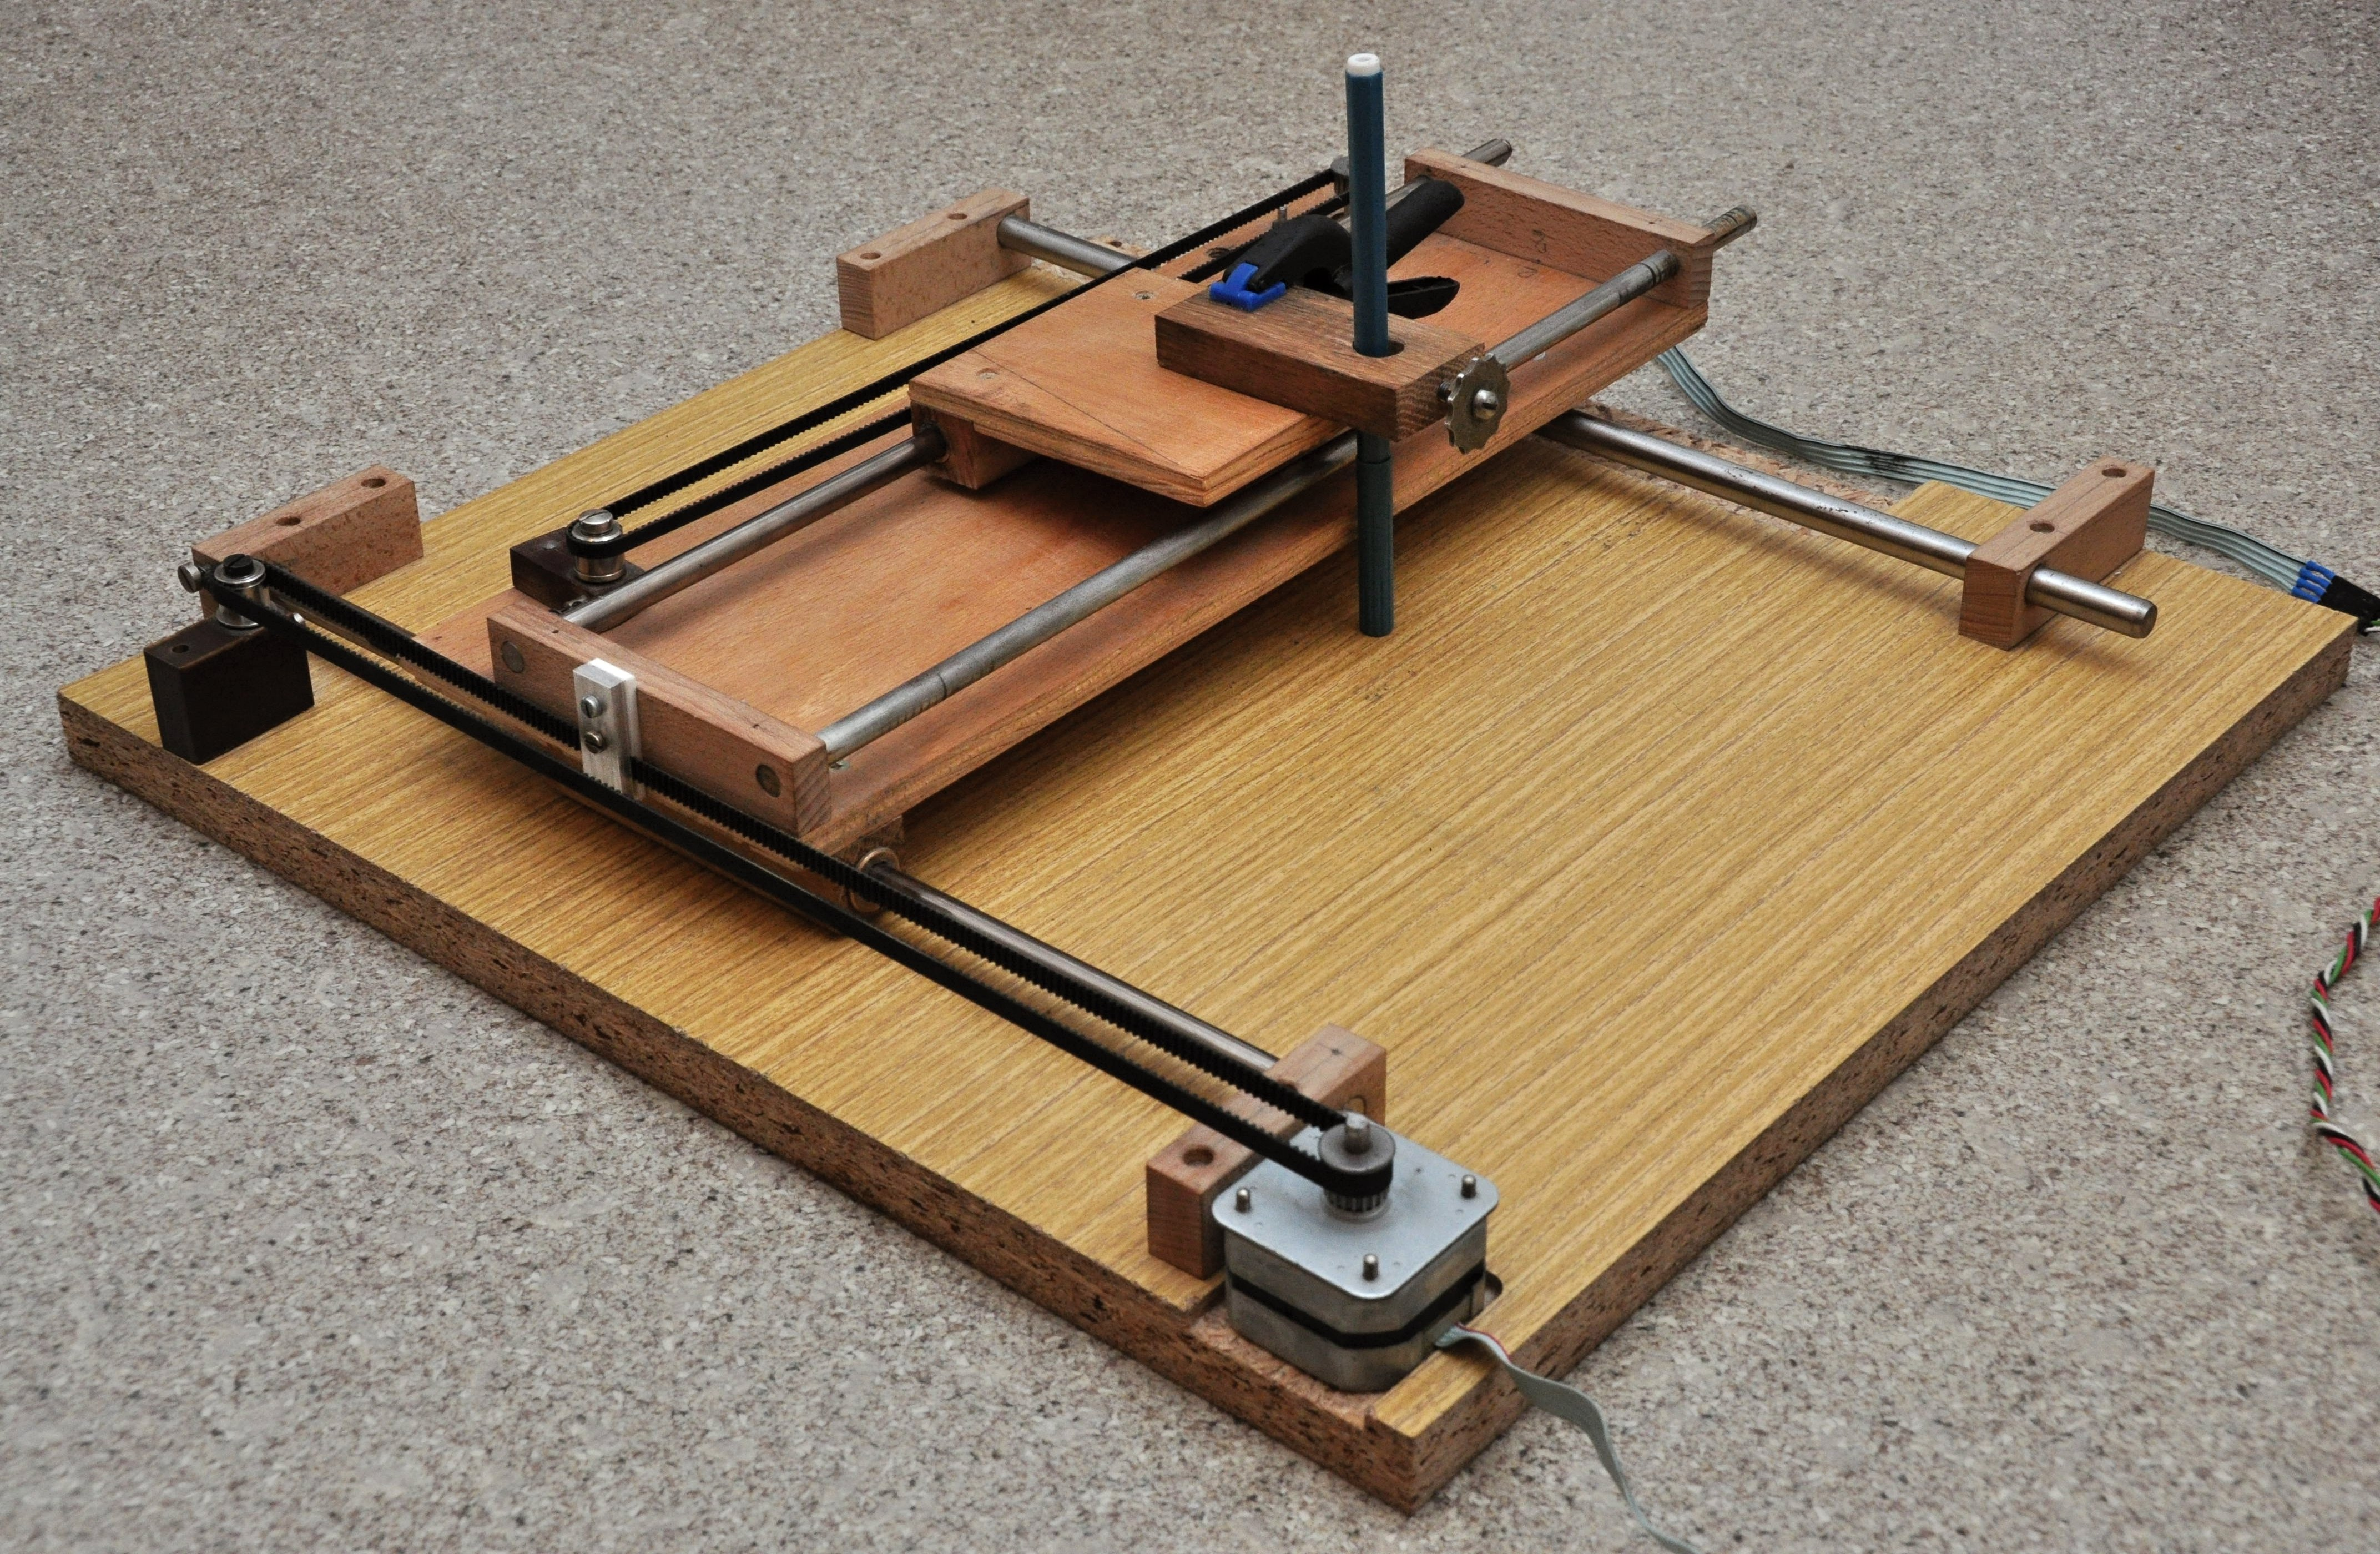
\includegraphics[width=0.8\textwidth]{img/plotter.jpg}
		\caption{Fotografie plotteru, na kterém byl systém testován}\label{fot:plotter}	
	\end{figure}
	
	\begin{figure}[h]
		\centering
		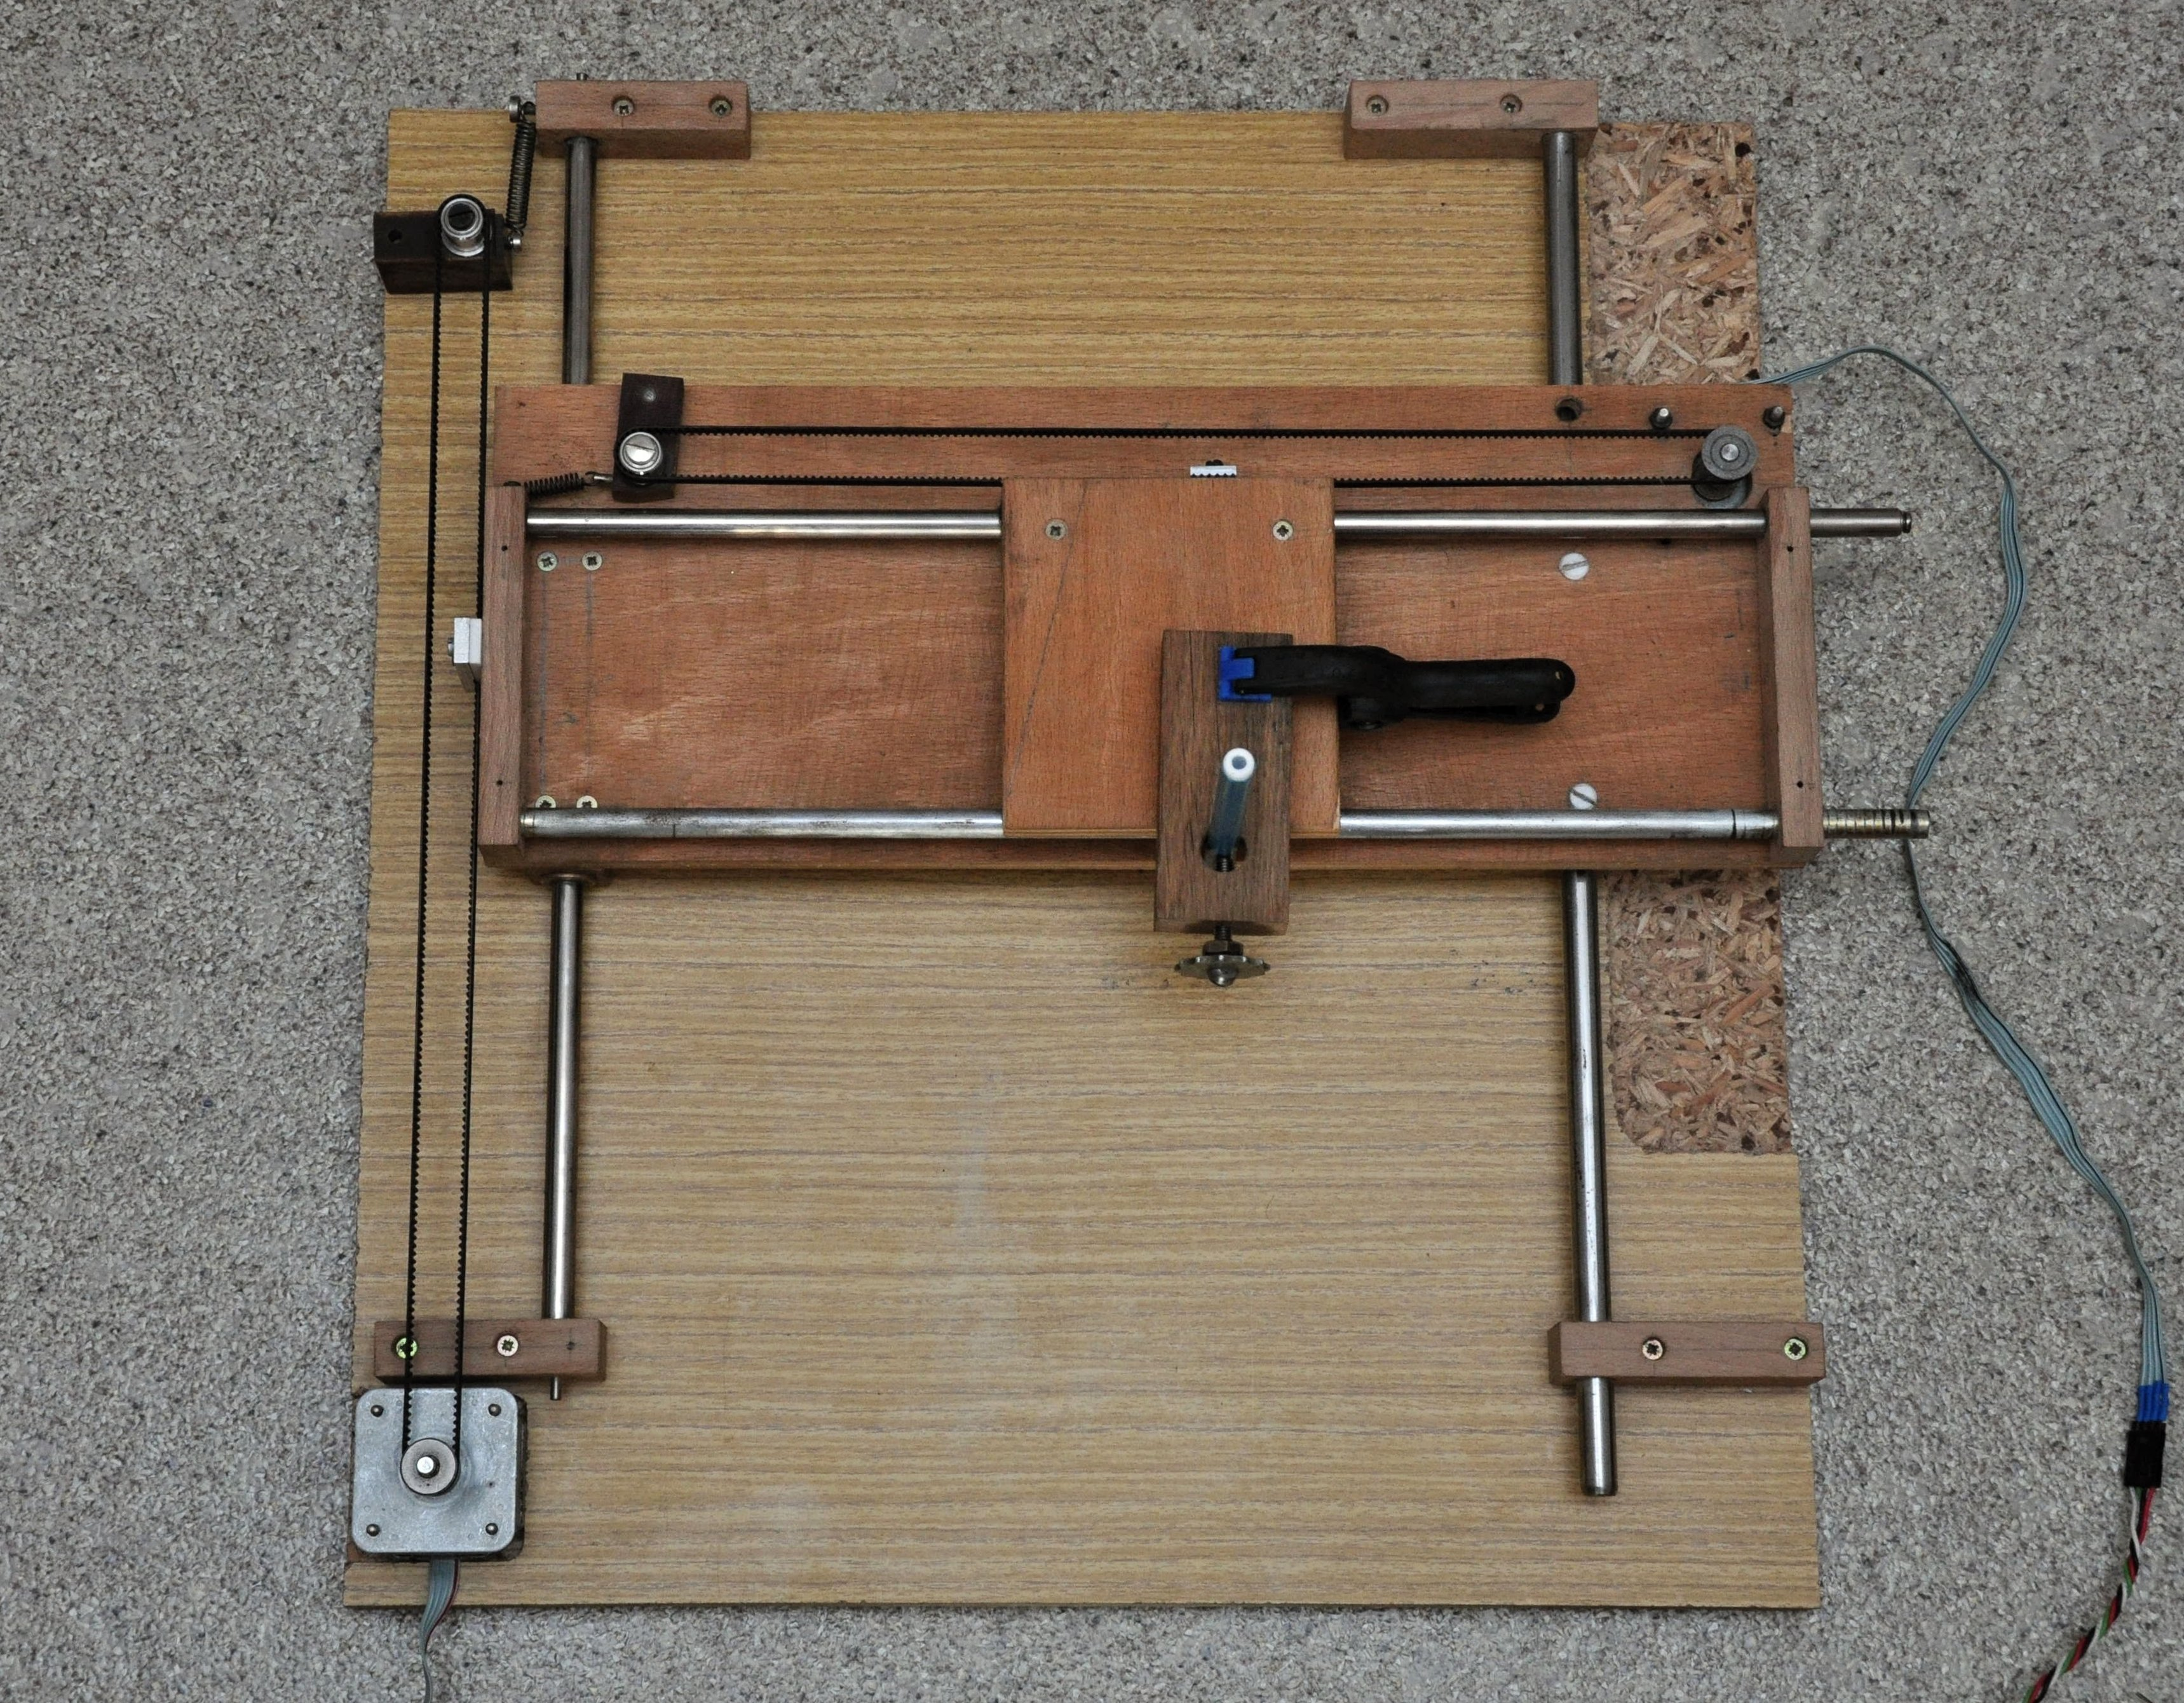
\includegraphics[width=0.8\textwidth]{img/plotter2.jpg}
		\caption{Fotografie plotteru, na kterém byl systém testován}\label{fot:plotter2}	
	\end{figure}
	
	Motory jsou řízeny čínskými \uv{no-name} jednoosými drivery postavenými na integrovaném obvodu Toshiba TB6560\cite{TB6560}. Mezi uživateli C-N-C.cz fóra se běžně označují jako \uv{čínská zelená jednoosá deska}. Existuje více mutací tohoto driveru, pro jeho přesnou identifikaci přikládám fotografii (obrázek \ref{fot:tb6560}). Tyto drivery jsou řízeny step-dir signálem.
	
	\begin{figure}[h]
		\centering
		\includegraphics[width=0.8\textwidth]{img/tb6560.jpg}
		\caption{Fotografie použitých driverů krokových motorů}\label{fot:tb6560}	
	\end{figure}
	
\chapter{Software pro interpolátor}

	Software pro interpolátor je primárně závislý na příchozí USB komunikaci a~interpolaci. Veškerou sérii úkonů jsem se rozhodl rozdělit do jednolivých komponent. Komponenty nejsou reprezentovány objekty, jelikož software je napsán v~jazyce C. Jelikož existuje pouze jediná instance od~každé komponenty, rozhodl jsem se každou komponentu reprezentovat jako soubor globálních funkcí pracujících nad svými globálními proměnnými.
	
	Rozvržení a~provázání jednotlivých komponent je znázorněno na schématu \ref{nak:rozvrzeni}.
	
	\begin{figure}[h]
		\centering
		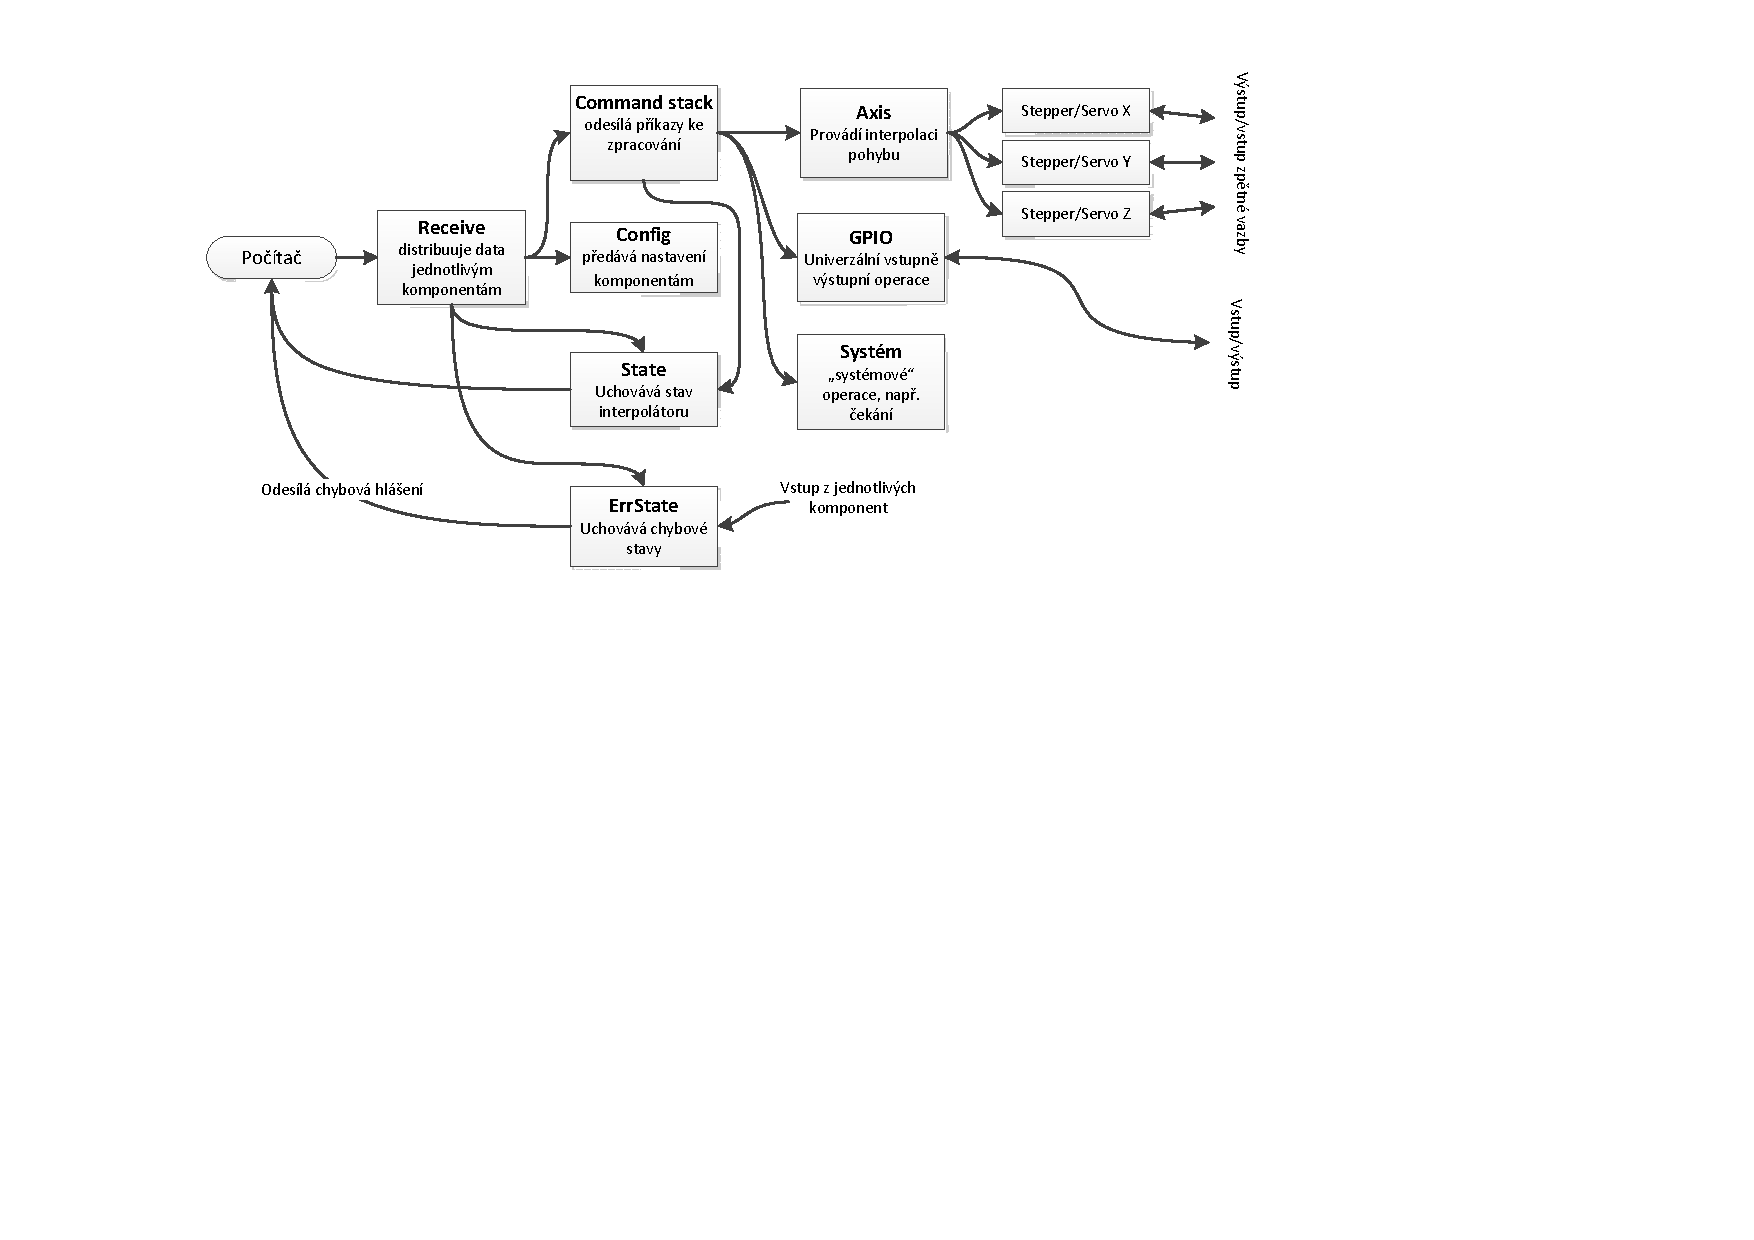
\includegraphics[width=1\textwidth]{img/rozvrzeni2.pdf}
		\caption{Schéma znázorňující rozvržení softwaru pro interpolátor}\label{nak:rozvrzeni}	
	\end{figure}
	
	Základní komponentou celé aplikace je komponenta {\tt Receive}. Tato komponenta zachytává přícházející pakety z~USB, skládá je dohromady a~nasledně tato přijatá data předává dále příslušným komponentám.
	
	Komponenta {\tt Config} příjímá zprávy týkající se nastavení a~na základě přijatých dat volá funkce pro nastavení příšlušných komponent.
	
	Komponenta {\tt State} uchovává informace o současném stavu interpolátoru a~podává zpětnou vazbu počítači. Obdobně komponenta {\tt ErrState} uchovává informace o chybovém stavu jednotlivých komponent a~podává zpětnou vazbu.
	
	Jednou z~nejdůležitějších komponent je {\tt CommandStack}. Tato komponenta přebírá veškeré příkazy pro stroj a~dle příznaku je buď řadí do fronty a~postupně vykonává nebo je vykoná přímo hned po přijetí. Příkazy pohybu zpracovává komponenta Axis, která provádí samotnou interpolaci. Zbývající dvě komponenty ({\tt GPIO} a~{\tt Global}) zpracovávají ostatní druhy příkazů -- např. prodlevu v~programu a~podobně.
	
	\section{Implementace USB a~komunikační protokol}
	Pro komunikaci mezi počítačem a~interpolátorem  používám integrovanou periférii v~mikrokontroléru. Pro její obsluhu jsem použil knihovnu dodávanou výrobcem -- STMicroelectronics -- USB Host-DeviceLibrary.
	
	Jelikož počítač umí v~USB komunikaci vystupovat pouze jako host, nakonfiguroval jsem kit jako device. Mým cílem bylo vytvořit vendor-defined device, které bude kromě control enpointu pro komunikaci využívat jeden vstupní a~druhý výstupní bulk endpoint -- tedy bude tvořit sériovou linku. Kit s~počítačem komunikuje rychlostí Full Speed (pro rychlost High Speed není na kitu příslušné PHY). Délku paketu jsem použil nejdelší možnou pro Full Speed komunikaci -- 64 bytů.
	
	Jelikož jsem měl problémy s nastavením projektu tak, aby se knihovna pro obsluhu USB periférie zkompilovala, vyšel jsem pro mou aplikaci z~projektu vytvořeného v~článku \uv{Začínáme s~STM32F4Discovery 7}\cite{mcu} od~uživatele s~přezdívkou Mard na serveru mcu.cz. Vstupní projekt jsem upravil tak, aby se zařízení tvářilo jako vendor-defined. O této úpravě a~mém prvním sestrojeném demu USB komunikace byl napsán článek na témže serveru\footnote{\url{http://mcu.cz/comment-n2904.html}}.
	
		\subsection{Komunikační protokol a~komponenta Receive}\label{kap:protokol}
		Jak vyplývá z~hiearchie jednotlivých komponent, komunikační protokol je vrstvený. V~nejvyšší vrstvě, kterou zpracovává komponenta {\tt Receive}, je ošetřeno rozdělení dat do více paketů (v~případě, že celková délka dat přesáhne 64 bytů). Veškerá komunikace probíhá binárně -- jednak abych ušetřil přenášená data, tak také, aby zpracování dat v~interpolátoru proběhlo co nejrychleji. Pokud budu čísla posílat v~binárním tvaru (což si můžu dovolit, jelikož platforma x86, resp. x64, je little-endian a~platforma ARM umí pracovat v~obou režimech -- little i big-endian\cite{wiki:end}), tak mi stačí pouhé ukládání dat a~nemusím parsovat textový formát.
		
		První byte prvního přijatého paketu obsahuje informaci o počtu paketů, do kterých je rozdělena právě příjímaná zpráva. Za tímto bytem následuje další byte, který definuje, které komponentě je zpráva určena. Seznam těchto kódů je definován v~hlavičkovém souboru {\tt CommunicationEnumerations.h}. Všechny pakety, které jsou přijaty, jsou předány funkci ProcessPacket. Tato funkce při přijetí prvního paketu vyčte délku zprávy $n$ v~paketech, nakopíruje ji do bufferu a~dalších $n-1$ přijatých paketů nakopíruje do bufferu za sebou. Jakmile je přijato všech $n$ paketů, zavolá funkci DistributeData, která předá přijatou zprávu dalším komponentám (na~základě druhého bytu).
		
		Každá komponenta definuje svou funkci ProcessMessage (tedy např. \texttt{CommandStackProcessMessage}), která zajistí zpracování zprávy dané komponenty. Tvar zprávy pro dané komponenty popisuji v~následujících sekcích.
		
		Pro komunikaci s~počítačem (pro zpětnou vazbu) je použit stejný princip na rozdělení zprávy do paketů. Druhý byte zprávy však nyní neurčuje danou komponentu (tato hiearchie na straně počítače neexistuje), nýbrž identifikátor zprávy. Všechny možné zprávy pro počítač jsou definovány v~hlavičkovém souboru {\tt MessageCodeToPC.h}.
		
	\section{Komponenta CommandStack}
	
	Komponenta {\tt CommandStack} má za úkol spouštět přijaté příkazy. Název této komponenty jsem bohužel zvolil jako trochu zavádějící. CommandStack reprezentuje datový typ fronty -- příkaz přijatý jako první se vykoná jako první.
	
	Příkazy jsou dvojího druhu -- jedny jsou určeny pro okamžité vykonání po jejich přijetí a~druhé jsou prvně umístěny do~bufferu a~postupně se vykonávají. {\tt CommandStack} je tedy implementován jako kruhový buffer. Do~tohoto bufferu jsou ukládány prvky typu {\tt CommandStruct}. Tato struktura reprezentuje jakýkoliv vykonatelný příkaz. {\tt CommandStack} také udržuje informace o~aktuálně vykonávaném a~posledním vykonaném příkazu.
	
	Rozhraním pro tuto komponentu je funkce StartPerforming. Tato funkce je po inicializaci všech komponent po startu interpolátoru volána v~nekonečné smyčce. V~této funkci je vždy vyjmut z~bufferu první příkaz a~je poslán ke zpracování.
	
		\subsection{Struktura CommandStruct}
		Struktura CommandStruct je definována následně:
		\begin{verbatim}
			typedef struct
			{
			    uint8_t receiver;//Receiver component for command
			    uint8_t type;//Type of command
			    CommandID ID;//Unique ID for command
			    union
			    {
			        uint32_t delay;//Delay in ms for waiting
			        uint8_t LED;//Led argument for GPIO
			        AxisLine line;//line argument for Axis component
			        AxisSine sine;//sine arguments for Axis component
			        AxisCircle circle;//circle argument for Axis component
			    };
			}	CommandStruct;
		\end{verbatim}
		V první části struktury jsou deklarovány členy, které jsou společné pro všechny příkazy. Mezi ně patří cílová komponenta, typ příkazu (enumerace pro tyto členy jsou opět definovány v~souboru {\tt CommunicationEnumerations.h}) a~ID každého příkazu. V~druhé části jsou pak v~unionu uloženy datové struktury pro jednotlivé typy příkazů.
		
		{\tt ID} je definováno jako 32-bitové neznaménkové číslo. Každý příkaz má jedinečný identifikátor přidělený počítačem -- používá se např. když interpolátor posílá počítači zprávu, který příkaz je právě vykonáván. Identifikátory není třeba recyklovat -- pokud by každou milisekundu byl vykonán jeden příkaz, k~přetečení tohoto datového typu by došlo za 49 dní, což je dostatečná rezerva.
		
		\subsection{Zpracování zpráv}
		
		CommandStack příjmá následující zprávy:
		
		\paragraph{COMSTACK\_RET\_SPACE}
		 se dotazuje na prázdné místo v~bufferu. Nemá žádné parametry. Odpovědí je {\tt COMSTACK\_FREE\_SPACE\_MESS}, která vrací 16-bitové číslo vyjadřující počet prázdných míst v~bufferu.
		
		\paragraph{COMSTACK\_ADD\_COM}
		 přidává do bufferu příkazy. Zpráva je složena z~8-bitového čísla určující počet zpráv k~přidání. Za ním následuje $n$ příkazů v~podobě {\tt CommandStruct}. Pokud není dostatek volného místa v~bufferu, nastaví se chybový stav {\tt ERR\_COMSTACKOWERFLOW} a~odešle se zpráva počítači.
		 
		\paragraph{COMSTACK\_LAST\_COM\_ID}
		  se dotazuje na ID posledního vloženého příkazu. Odpovědí je {\tt COMSTACK\_LAST\_ID}, která vrací ID posledního příkazu.
		  
		\paragraph{COMSTACK\_LAST\_ITEM\_PROC}
		 vrací identifikátor posledního úspěšně dokončeného příkazu. Odpovědí je {\tt LAST\_PROC\_ITEM\_STACK}, která vrací ID posledního příkazu.	
		 
		\paragraph{COMSTACK\_CURRENT\_ITEM\_PROC}
		 vrací identifikátor právě prováděného příkazu. Odpovědí je {\tt CUR\_PROC\_ITEM\_STACK}, která vrací ID posledního příkazu.	
		  
		\paragraph{COMSTACK\_CLEAR}
		 vyprázdní celý buffer.
		
		\paragraph{COMSTACK\_START}
		 spustí vykonávání příkazů v~bufferu.
		 
		\paragraph{COMSTACK\_PAUSE}
		 zastaví vykonávání příkazů v~bufferu.		 
		
		
	\section{Komponenta Axis}
	
	Komponenta {\tt Axis} vykonává provádění veškerých příkazů pro pohyb. V~této komponentě jsou definovány buffery, které uchovávají aktuální \uv{virtuální} pozici všech os. Na základě obsahu těchto bufferů řídí komponenta {\tt  Stepper}, popř. {\tt Servo}, drivery pohonů.
	
	Interpolace probíhá v~předem dané obnovovací frekvenci. To má na starosti timer {\tt TIM14}, který na základě nastavení, které je posláno z~počítače, pravidelně volá funkci {\tt UpdatePosition} pro vykonání dalšího kroku interpolace.
	
	Příkaz pro pohyb vyvolává komponenta {\tt CommandStack}, která volá funkci {\tt ProcessAxisCommand}. Tato funkce jako argument přebírá strukturu {\tt CommandStruct}. Na základě jejího obsahu připraví funkce {\tt ProcessAxisCommand} příslušný druh interpolace. Funkce poté před svým ukončením čeká, než funkce {\tt UpdatePosition} nastaví příznak označující dokončení pohybu.
	
		\subsection{Použití datového typu float}
		Před implementací této komponenty bylo důležité vhodně vybrat datové typy, ve kterých budou probíhat interpolační výpočty. Ačkoliv jsem zvažoval použití celočíselných datových typů a~následnou implementaci fixed-point aritmetiky, rozhodl jsem se nakonec použít čísla s~plovoucí desetinnou čárkou -- konkrétně datový typ {\tt float}.
		
		Čísla s~plovoucí desetinnou čárkou se pro podobné výpočty zpravidla nepoužívají, jelikož při jejich nesprávném použití můžou vznikat velké chyby a~práce s nimi na mikrokontrolérech bývá pomalá. Jelikož však mnou vybraný mikrokontrolér disponuje hardwarovou FPU, je práce s~datovým typem float téměř stejně rychlá jako s~celočíselným datovým typem. Navíc nemusím řešit změnu řádu při operacích jako je násobení a~dělení, či operace se dvěma čísly v~rozdílných řádech. Veškeré výpočty, které provádím, jsou počítány absolutně -- jejich vstupem jsou předem daná přesná data, nikdy se nezakládají na dříve vypočtené hodnotě -- výpočty tedy nejsou iterativní. V~případě interpolace nepřičítám k~aktuální pozici změnu, ale do bufferu ukládám součet počáteční pozice a~uražené dráhy.
		
		Existují však případy, kdy se nelze vyhnout iteračnímu výpočtu -- jedním z~případů je postupné obnovování hodnoty aktuálního času, kdy se k~proměnné přičítá velmi malá hodnota. V~tomto případě uchovávám a~pracuji s~hodnotou času jako s~celočíselným typem a~až těsně před použitím ve výpočtu převedu celočíselný datový typ na float. Stejně tak pracuji s~uloženou pozicí krokového motoru.
		
		\subsection{Implementace funkce sinus}
		
		Celý fyzikální model je založen na funkcích sinus a~cosinus. Tyto funkce jsou ve standardní knihovně implementovány za pomoci řad. Tato implementace je přesná, avšak velmi pomalá. Rozhodl jsem se proto naimplementovat tyto funkce pomocí vyhledávací tabulky.
		
		Mou prioritou bylo dosažení co nejrychlejšího výpočtu a~rozumné přesnosti. Jelikož má mnou vybraný mikrokontrolér dostatek flash paměti, připravil jsem si tabulku obsahující hodnoty pro kladnou půlvlnu sinu po krocích $\frac{\pi}{4000}$. Tato tabulka zabírá v~paměti necelých 16~kB.	Funkce cosinus je realizována za pomoci posunu v~této tabulce.
		
		Touto tabulkou jsem získal velmi rychlý výpočet pro hodnoty sinu s~dostatečnou přesností.
	
		\subsection{Lineární interpolace}
		Lineární interpolace je využita pro realizaci funkcí G00 a~G01, popř. jako část cyklů (např. G73 vrtací cyklus)\cite{gcode}. Tato interpolace je předávána jako prvek line struktury CommandStruct. Line je typ AxisLine, který je definován následovně:
		\begin{verbatim}
		typedef struct
		{
		    float axis[3];
		    float v0, v, vb;
		    float As, Ab;
		}	AxisLine;
		\end{verbatim}
		Pole {\tt axis} reprezentuje novou polohu os, neboli cílový bod interpolace ze současné pozice. Členy {\tt v0, v, vb} reprezentují počáteční rychlost, respektive cílovou a~brzdnou. {\tt As a~Ab} reprezentují zrychlení použité pro rozjezd a~brzdění. Veškeré jednotky, které stroj používá, používají jako jednotku délky 1~mm, tedy rychlost je v~jednotkách 1~mm$\cdot$s$^{-1}$, zrychlení v~jednotkách 1~mm$\cdot$s$^{-2}$.
		
		Tato struktura je zpracována funkcí {\tt ProcessAxisLine} (voláno funkcí {\tt ProcessAxisCommand}). Tato funkce připraví nezbytná data tak, aby interpolace každé osy mohla probíhat nezávisle na~ostatních. V~této funkci nejprve určím vektor ve směru pohybu jako rozdíl konečného a~počátečního bodu. Tento vektor znormalizuji a~jeho vynásobením se zadaným zrychlením dostanu maximální velikost zrychlení pro každou osu. Stejnou proceduru provedu i s~jednotlivými rychlostmi.
		
		Nyní dopočítám dle odvozených vztahů v~kapitole \ref{kap:pohybpousecce} čas a~dráhu nutnou k~rozjezdu. Na~základě těchto dvou údajů poté určuji v~jaké fázi se pohyb nachází, abych mohl jeho polohu počítat dle správných vztahů.
		
		Pro interpolaci využívám vztah pro dráhu (vztah \ref{rov:lindraha}), který mi vyjadřuje okamžitou vzdálenost od~počátku pohybu. V tomto vztahu je spousta konstantních výrazů pro daný pohyb, proto si tyto konstanty před začátkem pohybu předpočítám, abych je nemusel při každém kroku interpolace znovu počítat.
		
		Všechny předpočítané údaje jsou uloženy ve dvou strukturách. Struktura {\tt AxisMovementLineCommon} reprezentuje data shodná pro všechny osy.
		\begin{verbatim}
			typedef struct
			{
			    float T, TB, t;
			}	AxisMovementLineCommon;
		\end{verbatim}
		Zde {\tt T} vyjadřuje čas nutný k~rozjezdu, {\tt TB} čas nutný ke zbrzdění a~{\tt t} čas, jak dlouho trvá pohyb konstantní rychlostí.
		
		Struktura {\tt AxisMovementBufferLine} je přiřazena ke každé ose a~uchovává jejich specifická data.
		\begin{verbatim}
		typedef struct
		{
		    float* position;
		    float ATpi, ATpiB;
		    float start, constant, brake, end;
		    float v, v0;
		}	AxisMovementBufferLine;
		\end{verbatim}
		{\tt position} je ukazatel na float uchovávající aktuální pozici osy, {\tt ATpi} ({\tt ATpiB}) je předpočítaná hodnota výrazu $\frac{AT}{\pi^2}$ (respektive jeho varianty pro brzdění). {\tt start, constant, brake, end} znamenají postupně: pozici osy pro počátek; místo, odkud se osa pohybuje konstantní rychlostí; místo, odkud začíná osa brzdit; cílová pozice. {\tt v} reprezentuje konstantní rychlost, {\tt v0} počáteční.
		
		Interpolace probíhá následovně. Prvně se pro všechny osy inkrementuje čas. Dále probíhá interpolace pro každou osu samostatně -- na základě času se určí, v~jaké fázi se pohyb nachází. Následně se spočte jeho dráha podle vztahu \ref{rov:lindraha} a~přičte se k~ní počátek celého pohybu. Pokud na dané ose došlo ke změně polohy, je zavolána fukce NotifyMovement, která aktualizuje polohu pohonu.
		
		Jakmile čas dosáhne zadané hranice, je nastaven příznak dokončeného pohybu a~funkce {\tt ProcessAxisLine} se ukončí.
		
		\subsection{Oblouková interpolace}\label{kap:oblinter}
		
		Oblouková interpolace je využita pro realizaci funkcí G02, G03, G12 a~G13\cite{gcode}, popř. je využita při cyklech a~kompenzaci nástroje. Tato interpolace má podobnou mechaniku a~hiearchii jako lineární, proto se v~následujícím textu zaměřím pouze na rozdíly.
		Příkaz pro obloukovou interpolaci je předáván jako prvek {\tt circle} struktury {\tt CommandStruct}. {\tt circle} je typ {\tt AxisCircle}, který je definován následovně:
		\begin{verbatim}
		typedef struct
		{
			    float B[3], C[3];
			    float v, v0, vb;
			    float As, Ab;
		}	AxisCircle;
		\end{verbatim}
		{\tt B} a~{\tt C} zde označují body; B je koncový bod oblouku a~C je bod ležící kdekoliv na něm (s~podmínkou, že současná poloha stroje a~body B, C nesmí ležet na jedné přímce). {\tt v, v0, vb} opět označují příslušné rychlosti, {\tt As} a~{\tt Ab} opět označují použitá zrychlení.
		
		Zde je nutno podotknout, že současná podoba interpolace je v~rozporu se standardem G-kódu. Můj kód je schopný projet kruhový oblouk ležící v~obecné rovině (proto se zadává za pomoci tří bodů), zatímco G-kód definuje jako přípustné roviny pouze XY, XZ a~YZ. Tato chyba vznikla mým prvopočátečním špatným pochopením standardu. Dále dle standardu je možné pomocí kruhové interpolace interpolovat šroubovici. Toho lze docílit zadáním z-ové (respektive y-ové nebo x-ové) souřadnice koncového bodu tak, aby ležel mimo danou rovinu. Tento druh interpolace můj systém zatím nezvládá a~chybně se snaží ze zadaných údajů sestrojit kružnici v~obecné rovině. Z~tohoto důvodu probíhá samotná interpolace zbytečně složitě.
		
		Výše uvedená struktura je zpracovávaná funkcí {\tt ProcessAxisCircle} (volané funkcí {\tt ProcessAxisCommand}). V~této funkci jsou připravena veškerá data. Kružnice je interpolována společně pro všechny osy -- výstupem interpolace je úhlová dráha (v~kódu označována jako {\tt alph}a), na~základě které se dopočítává poloha jednotlivých os.
		
		Funkce {\tt ProcessAxisCircle} nejprve dopočte střed kružnice na základě jejích třech bodů (sestrojením normálového vektoru roviny kružnice, díky němuž je možné vytvořit osy tětiv ze~tří bodů a~nalezením průsečíků těchto os). Poté připraví data. Příjatá data ve struktuře {\tt AxisCircle} vyjadřují obvodové hodnoty. Jak jsem napsal v~předchozím odstavci, pro mou interpolaci potřebuji úhlové hodnoty. Proto všechny hodnoty rychlostí a~zrychlení před použitím vydělím poloměrem oblouku, čímž získám úhlovou rychlost a~úhlové zrychlení, na základě nichž dopočítám potřebné konstanty stejně jako v~případě lineární interpolace (nyní však pouze pro jednu \uv{osu} -- úhlovou).
		
		Po dopočítání úhlové dráhy potřebuji tuto dráhu převést na kružnici v~kartézských souřadnicích. Pro tento převod používám parametrickou rovnici kružnice v~obecné rovině (vztah \ref{rov:kruznice}\cite{kruznice})
		\begin{equation}
		\label{rov:kruznice}
		\vec{P} = R\;\vec{u}\cos(t) + R\sin(t) \;\;\vec{n}\times\vec{u} + \vec{c}
		\end{equation}
		V tomto vztahu $\vec{P}$ je polohový vektor hledaného bodu, $R$ poloměr oblouku, $t$ parametr, $\vec{n}$ jednotkový vektor kolmý na rovinu kružnice, $\vec{u}$ jednotkový vektor směřující ze středu k~počátečnímu bodu oblouku a~$\vec{c}$ polohový vektor středu kružnice. Vektorovou rovnici jsem si pro potřeby převodu rozdělil na jednotlivé osy, jim předpočítal konstantní hodnoty a~jako paramet předávám okamžitou úhlovou dráhu.
		
		Potřebná data jsou uložena obdobně jako u~lineární interpolace v~následujících strukturách:
				\begin{verbatim}
				typedef struct
				{
				    float w, w0;
				    float alpha;
				    float constant, brake, end;
				    float ATpi, ATpiB, T, TB;
				}	AxisMovementCircleCommon;
				
				typedef struct
				{
				    float* position;
				    float final;
				    float crossProduct, center, R, u;
				}	AxisMovementBufferCircle;
				\end{verbatim}
		
		Vynechané části průběhu interpolace probíhají podobně jako u lineární, proto je dále nepopisuji.
		
		\subsection{Interpolace ideální křivky}
		V kódu lze spatřit i odkazy na interpolaci ideální křivky z~kapitoly \ref{kap:krivka}. Jak jsem v~ní zmínil, s~křivkou jsem počítal pouze na~počátku a~v~pozdější fázi vývoje jsem se ji rozhodl vypustit. Interpolace této křivky je tedy ve funkčním stavu, avšak na této křivce není omezen ryv a~neexistuje možnost, jak křivku vložit z~G-kódu (není podporovaná na straně počítače). V~kódu interpolátoru jsem ji však do budoucna pro případnou plnou implementaci ponechal.
		
	\section{Komponenty Movement a~Stepper}
	
	Komponenta {\tt Movement} zajišťuje převod pozice jednotlivých os na výstupní signál pro drivery. V~začátcích projektu jsem měl v~plánu implementovat jak step-dir řízení v~podobě komponenty {\tt Stepper}, tak i PID smyčku se zpětnou vazbou pro přímé řízení servomotoru v~podobě komponenty {\tt Servo}. V~současnosti je implementována pouze komponenta {\tt Stepper} a~interpolátor tedy umí generovat pouze step-dir signál. Úkolem komponenty {\tt Movement} je zajistit jednotné rozhraní pro generování výstupních signálů pro komponentu {\tt Axis}, která volá její funkci {\tt NotifyMovement}.
	
	Pro každou osu je vytvořen jeden prvek následující struktury:
	\begin{verbatim}
	typedef enum {STEPPER = 1, SERVO = 2, UNUSED = 0} MovementType;
	
	typedef struct
	{
	    MovementType type;
	    union
	    {
	        Stepper stepper;
	        Servo servo;
	    };
	} MovementStruct;
	\end{verbatim}
	Při zavolání funkce {\tt NotifyMovement} (tedy když se změnila poloha osy), je na základě členu type rozhodnuto, zdali se bude volat funkce pro upozornění komponenty {\tt Stepper} nebo {\tt Servo}.
	
	To, která osa bude obsahovat komponentu {\tt Stepper} a~která {\tt Servo}, je určeno nastavením z~počítače. Toto nastavení je provedeno pomocí příchozí zprávy {\tt CONFIG\_MOVEMENT\_SETTYPE}. První byte této přijaté zprávy určuje index osy, pro kterou se nastavuje typ, a~druhý byte určuje druh generátoru výstupního signálu (Stepper/Servo) pro tuto osu. Druhou zprávou, kterou je nutno poslat, je zpráva {\tt CONFIG\_MOVEMENT\_INDIVIDUAL} předávající dané ose, respektive generátoru, jeho příslušná nastavení. První byte této zprávy určuje index osy a~za ním následují konfigurační data (konfigurační zpráva), která jsou předána již příslušné komponentě ke zpracování.
	
		\subsection{Komponenta Stepper}
		Komponenta {\tt Stepper} sloužící ke generování step-dir signálu je reprezentována následující strukturou:
		\begin{verbatim}
		typedef struct
		{
		    uint32_t mmPerStep;
		    int32_t position;
		    uint8_t pulsePin;
		    GPIO_TypeDef* GPIO;
		    uint16_t directionPin;
		    bool inverted;
		    bool lastDirection;
		}	Stepper;
		\end{verbatim}
		Tato struktura uchovává veškerá data a~nastavení. Člen {\tt mmPerStep} vyjadřuje vzdálenost, o kterou je posunuta osa při jednom kroku. Tato hodnota je uložena v~desetitisícinách milimetru ($10^{-4}~$mm). Člen {\tt position} vyjadřuje současnou pozici osy v~desetitisícinách milimetru (tedy maximální délka osy je $\pm214$~metrů). Člen {\tt pulsePin} je index výstupního pinu pro komponentu {\tt PulseGenerator}, na kterém probíhá generování signálu step. Členy {\tt GPIO} a~{\tt directionPin} určují výstupní pin pro signál dir. Člen {\tt inverted} určuje, zda-li je třeba prohodit směr otáčení osy. Člen {\tt lastDirection} není nastavením, nýbrž ukládá směr pohybu při poslední aktualizaci pohybu.
		
		Pokud nastane změna pohybu osy, je skrz univerzální rozhraní komponenty {\tt Movement} zavolána funkce komponenty {\tt Stepper NotifyStepper}. Tato funkce nejprve zjistí odchylku fyzické pozice osy (na základě členu {\tt position} ve struktuře {\tt Stepper}) od~pozice osy vypočtené komponentou {\tt Axis}. Pokud je tato odchylka větší než velikost jednoho kroku (člen {\tt mmPerStep}), zjistí jednotka směr (tedy polaritu signálu dir) a~za pomoci komponenty {\tt PulseGenerator} vygeneruje signál step. Poté přičte, či odečte délku jednoho kroku od~aktuální pozice.
		
		\subsection{Komponenta PulseGenerator}
		
		Komponenta {\tt PulseGenerator} má za úkol generovat pulzy. Původní myšlenka byla, aby byla schopna generovat pulzy libovolné délky v~daném rozsahu s~největší možnou přesností. Toho jsem chtěl docílit použitím timerů {\tt TIM3} a~{\tt TIM12} v~PWM módu. V~PWM módu generují timery na pinech {\tt PA6, PA7, PB0, PB1} a~{\tt PB14, PB15} PWM signál\cite{refman}, jehož střídu lze určit hodnotou příslušných compare registrů. Frekvence PWM je dána předděličkou k~timeru. Procesor umí generovat přerušení při přetečení timeru\cite{refman}. Těchto vlastností jsem využil ke generování jednoho pulzu -- nastavil jsem si do fronty délku jednoho pulzu, při přetečení timeru jsem nastavil správnou hodnotu šířky pulzu a~PWM mód jsem spustil. Při opětovném přetečení jsem timer vypnul. Tím jsem docílil generování jednoho pulzu. V~průběhu testování se však ukázalo, že vznikají parazitní pulzy -- pohony dělaly kroky navíc. Podezříval jsem, že se díky vnořování přerušení nestíhá PWM mód v~čas vypínat -- tuto doměnku se mi však nepodařilo ověřit.
		
		Rozhodl jsem se proto oželet možnost generovat proměnlivou délku pulzu a~za pomoci timeru generovat pulz konstantní šířky. Bohužel při tomto generování pulzu vznikal stejný jev -- objevovaly se pulzy navíc. Snažil jsem se chybu objevit, avšak neúspěšně.
		
		Z nedostatku času a~díky nutnosti funkčnosti této komponenty (bez ní nelze řídicí systém testovat), jsem se uchýlil k~dočasnému hacku. Nyní generuji 100~ns pulz a~čekání zajišťuji sérií instrukcí nop. Nyní mi již nevznikají žádné parazitní pulzy. Toto řešení je dočasné a~mělo by být co nejdříve nahrazeno jiným.

	
	\section{Implementace ostatních komponent}
	V předchozích sekcích byly popsány nejdůležitější komponenty, které tvoří jádro celého interpolátoru. Tyto komponenty mají na starost pohyb stroje. G-kód však definuje další druhy příkazů, které se netýkají pohybu a~proto bylo nutné do návrhu přidat ještě dvě komponenty.
	
		\subsection{Komponenta GPIOControl}
		Tato kompenta má za úkol obsluhovat vstupy a~výstupy mikrokontroléru. Skrze ni by mělo být např. zapínáno vřeteno (funkce M03, M04\cite{gcode}). Záměrně byla tato komponenta navžena úzce spjatá s~hardwarem, aby si zachovala univerzálnost, a~tak bylo možné v~počítači co nejpodrobněji nakonfigurovat chování.
		
		Tato komponenta není zatím dokončena a~pro demonstrativní účely zatím umí ovládat jednotlivé LED na kitu, které jsem používal pro demonstraci funkčnosti.
		
		\subsection{Komponenty SystemComponents}
		{\tt SystemComponents} zastřešuje příkazy spíše systémového rázu, které nesouvisí s~výstupem. Příkladem takového příkazu (a zatím jediného implementovaného z této katogorie) je funkce prodlevy -- P parametr příkazů G-kódu\cite{gcode} realizován pomocí {\tt DelayComponent}.
		
		Prodleva je implementována pomocí přerušení {\tt SysTick} \cite{refman}. Frekvence tohoto přerušení byla nastavena na 1~kHz -- přerušení nastává každou milisekundu. {\tt DelayComponent} implementuje seznam až 32 prodlev. Pokaždé, když nastane přerušení, je hodnota každé prodlevy právě o~jednu milisekundu zmenšena. Jakmile dosáhne hodnota prodlevy nuly, je prodleva ze seznamu odstraněna a~je zavolána případná callback funkce.
	

\chapter{Software pro počítač}

	Jak jsem již zmínil v~kapitole \ref{kap:prostredky} (\nameref{kap:prostredky}), aplikace pro počítač je napsána v~jazyce C++ s~využitím prvků z~nového standardu C++11. Pro GUI jsem použil framework WxWidgets. V~následujícím textu záměrně vynechávám některé detaily implementace (především co se GUI a~výstavby aplikace týče), jelikož se jedná vesměs o~standardní postupy, a~zaměřuji se na specifika řídicího systému -- interpretaci G-kódu, výpočet rychlosti pro stroj a~následnou komunikaci s~interpolátorem.
	\section{Uživatelské rozhraní}
	Uživatelské rozhraní mé aplikace je tvořeno jedním oknem, rozděleným na tři panely (viz obrázek \ref{obr:okno}).
	\begin{figure}[h]
		\centering
		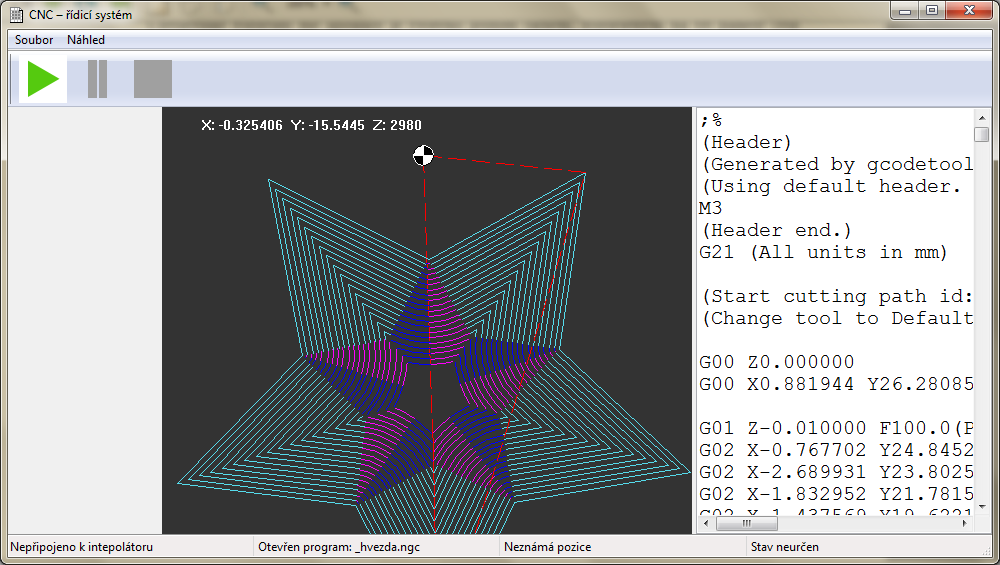
\includegraphics[width=0.99\textwidth]{img/okno2.png}
		\caption{Screenshot uživatelského rozhraní}\label{obr:okno}	
	\end{figure}
	
	Pravý panel zobrazuje aktuálně načtený program v~G-kódu a~za jeho běhu zvýrazňuje aktuálně prováděný řádek. Úplně levý panel zatím není využit, do budoucna by však měl zobrazovat další ovládací prvky a~informace.
	
	Prostřední panel zobrazuje náhled drah stroje. V~současné verzi zobrazuje pouze 2D náhled drah, které leží v~rovině XY. Náhled je možné libovolně posouvat myší a~kolečkem jej přibližovat/oddalovat. Do tohoto náhledu se také zobrazuje zpětná vazba z~interpolátoru (zvýrazňují se již projeté dráhy). Dráhy zadané přímo G-kódem se zobrazují barevně odlišené podle druhu interpolace (rychloposuv je naznačen přerušovaně). Barvy jednotlivých typů interpolace lze navolit v~konfiguračním souboru. Dráhy, které byly dopočteny (vznikly kompenzací nástroje), jsou zobrazeny bíle.
	
	Dole v~taskbaru aplikace jsou zobrazeny následující údaje: stav připojeno/odpojeno od~interpolátoru, otevřený program, okamžitá pozice os a~současný (chybový) stav interpolátoru.
	
	V~toolbaru se nacházejí tři tlačítka pro spuštění, pozastavení a~úplné zastavení běhu programu. V~menu aplikace Soubor lze otevřít program v~G-kódu. V~menu náhled je možné vypnout zobrazování již provedených pohybů strojem a~obnovit zobrazení náhledu drah.
	
	Uživatelské rzohraní je v~současném stádiu vývoje velmi chudé a~veškerá nastavení jak aplikace, tak interpolátoru jsou prováděna úpravou konfiguračního INI souboru. Aplikace využívá jediný konfigurační soubor {\tt settings.ini}. V tomto souboru jsou definovány jednotlivé sekce, obsahující příslušná nastavení.
	
	\section{Intepretace G-kódu}
	Jednou z~klíčových vlastností řídicího systému je parsování G-kódu na interní formát, se kterým lze uvnitř programu pracovat.
		\subsection{G-kód a~jeho formát}                        \label{kap:gcodeform}
		G-kód je univerzální jazyk pro programování CNC strojů\cite{wiki:gcode}. Syntaxe G-kódu je ralativně jednoduchá. Program je dělen na tzv. bloky. Blok je jeden řádek programu. V~každém bloku jsou uvedeny hodnoty jednotlivých registrů (A--Z). Registr G může být uveden vícekrát, čímž mu je přiděleno více hodnot\cite{wiki:gcode}. G-kód ignoruje mezery a~obecně jakékoliv bílé znaky. Program zpravidla začíná a~končí znakem procenta (\%). Komentáře v~G-kódu jsou umístěny do obyčejných jednoduchých závorek a~nesmí přesáhnout hranici jednoho bloku.
		
		Nejpoužívanějšími registry jsou registry G a~M, které uchovávají typ funkce k~vykonání. Ostatní registry slouží jako parametry těchto funkcí. Registry X, Y, Z uchovávají souřadnice lineárních os (koncové body). Vedle těchto registrů se používají i registry A, B, C pro polohu rotačních os, avšak jelikož můj interpolátor podporuje pouze 3 osy, nebudu tyto registry dále zmiňovat. Registry I, J, K a~R slouží pro zadávání parametrů obloukové interpolace. Registr F určuje rychlost stroje (posuv). Ostatní registry jsou méně používané, jejich kompletní seznam lze nalézt na stránkách \cite{wiki:gcode}.
		
		Seznam všech G-funkcí, které můj systém v~současné verzi podporuje, a~jejich popis je uveden v~tabulce~\ref{tab:funkce}.
		
		Funkce G zpravidla vykonávají pohyb stroje a~nastavují parametry. Funkce M mají speciální význam, který je dán specificky pro každý stroj. Existují však některé ustálené M-funkce (např. M03 pro zapnutí vřetena\cite{wiki:gcode}). Pokud je v~jednom bloku uvedeno více funkcí, určuje pořadí jejich vykonání stroj.
		
		G-kód podporuje i podprogramy, zápis matematických výrazů či polární zadávání souřadnic. Tyto funkce však dnes už nejsou (obvzláště v~hobby sféře) příliš rozšířené. Dříve podprogramy umožňovaly zkrácení programu a~jeho snažší zápis pro člověka. Tyto funkce však již dnes s~nástupem CAM programů nejsou zapotřebí. Proto jsem se tyto funkce rozhodl do mého systému neimplementovat.
		
		Některé hodnoty některých registrů si systém pamatuje do doby, dokud nejsou znovu nastaveny. Příkladem můžou být zadané cílové souřadnice, či posuv. Není tedy nutné zadávat pokaždé znovu všechny 3 souřadnice, stačí pouze ty, které se změnily. Také pokud byla použita funkce G01 (lineární interpolace), tak lze pro sérii pohybů po úsečce napsat pouze do prvního bloku G01 a~do dalších bloků uvést pouze souřadnice. Systém pak automaticky použije funkci G01.
		
		Část programu v G-kódu může vypadat následovně:
		\begin{verbatim}
		G00 X1	Y31 Z50
		G01 Z0.1 F100
		    X0.19 Y 29.58
		G02 X2.1 Y26.89 I6.64 J3.47
		    X5.53 Y25.61 I4.26 J6.16
		    X2.1 Y26.89 I6.64 J3.47
		\end{verbatim}
		
		\begin{table}
		    \begin{tabularx}{\textwidth}{|c|X|c|}
		        \hline
		        Funkce & Význam                                                                                                                                                                                                                                                                                               & Argumenty              \\ \hline \hline
		        G00    & Rychloposuv. Funkce není určená pro obrábění. Stroj nemusí pohyb interpolovat lineárně.                                                                                                                                                                                                              & X, Y, Z                \\ \hline
		        G01    & Lineární interpolace ze současné pozice na zadanou posuvem F                                                                                                                                                                                                                                         & X, Y, Z, F             \\ \hline
		        G02    & Oblouková interpolace ve směru hodinových ručiček. Oblouk je zadán současnou polohou a~koncovým bodem. Jeho střed je určen buď registry I, J, K, které určují odsazení středu od~počáteční polohy, nebo prametrem R učujícím poloměr oblouku. Učebnice G-kódu doporučují zadávání pomocí odsazení. & X, Y, Z, I, J, K, R, F \\ \hline
		        G03    & Oblouková interpolace proti směru hodinových ručiček. Zadáváno stejně jako G02                                                                                                                                                                                                                       & X, Y, Z, I, J, K, R, F \\ \hline
		        G20    & Nastaví pracovní jednotky na palce                                                                                                                                                                                                                                                                   & ~                      \\ \hline
		        G21    & Nastaví pracovní jednotky na milimetry                                                                                                                                                                                                                                                               & ~                      \\ \hline
		        G40    & Funkce zruší kompenzaci nástroje                                                                                                                                                                                                                                                                     & ~                      \\ \hline
		        G41    & Zapne kompenzaci nástroje doleva ve směru obrábění. Průměr nástroje je zadán jako D                                                                                                                                                                                                                  & D                      \\ \hline
		        G42    & Zapne kompenzaci nástroje doprava ve směru obrábění. Průměr nástroje je zadán jako D                                                                                                                                                                                                                 & D                      \\ \hline
		        G43    & Zapně kompenzaci délky nástroje kladného směru osy~Z. Délka nástroje je zadána jako H                                                                                                                                                                                                                 & H                      \\ \hline
		        G44    & Zapně kompenzaci délky nástroje do záporného směru osy~Z. Délka nástroje je zadána jako H                                                                                                                                                                                                             & H                      \\ \hline
		        G49    & Vypne délkovou kompenzaci nástroje                                                                                                                                                                                                                                                                   & ~                      \\
		        \hline
		    \end{tabularx}
		    \caption{Tabulka G-funkcí podporovaných mým systémem. Definice funkcí převzaty z~\cite{gcode}.}\label{tab:funkce}
		\end{table}
		
		\subsection{Interní formát a~třída GCodeInterpreter}
		Abych mohl G-kód dále zpracovat (dopočítat rychlost, provést korekce, odeslat do interpolátoru), musím jej neprve převést na interní formát mého programu, se kterým lze dobře pracovat.
		
		Veškeré zpracování G-kódu má na starosti třída {\tt GCodeInterpreter}. Tato třída implementuje veškerou funkcionalitu pro převod vstupního řetězce obsahujícího G-kód na příkazy pro interpolátor. Tento proces v~sobě zahrnuje i provedení korekcí nástroje a~výpočet rychlosti. Převedení G-kódu na výsledek je spuštěno funkcí {\tt ProcessString}. Tato metoda přebírá {\tt std::string}, který obsahuje G-kód. Výsledkem je seznam objektů pro vykreslení na obrazovce a~seznam připravených příkazů pro interpolátor. Třída {\tt GCodeInterpreter} v~sobě zahrnuje i načtení konfigurace týkající se zpracování z~daných konfiguračních souborů a~jejich následné předání příslušným metodám či objektům. Také uchovává stav jednotlivých parametrů v~průběhu převodu.
		
		\subsection{Převod G-kódu}
		Parsování G-kódu probíhá v metodě {\tt GCodeInterpreter::ParseCodeToPath} ve dvou krocích -- v~prvním kroku z~G-kódu vyčtu hodnoty jednotlivých registrů pomocí metody {\tt GCodeInterpreter::ParseGCodeLine}. Jelikož některé registry mohou obsahovat více hodnot (např. registr G), vrací tato funkce asociativní pole, kde je klíčem char označující registr a~hodnotou je seznam čísel s plovoucí desetinnou čárkou ({\tt std::map$<$char, vector$<$float$>>$}). V~druhém kroku jsou z~tohoto asociativního pole vybrány jednotlivé funkce a~jejich argumenty podle prototypů. To provádí metoda {\tt GCodeInterpreter::SeparateCommandsFromLine}. Zároveň tato metoda zajišťuje správné pořádí provádění funkcí v~případě, kdy je jich v~bloku uvedeno více.
		
		Metoda {\tt ParseGCodeLine} v~cyklu postupně načítá jeden znak ze stringu. Pokud je tento znak bílý, tak jej přeskočí. Pokud narazí na znak~\uv{{\tt (}}, začne načítat a~zahazovat další znaky, dokud nenarazí na znak~\uv{{\tt )}}. Pokud je načtený znak písmeno, načte pomocí třídy stringstream z~následujích znaků číslo a~uloží je do asociativního pole, které je na konci navráceno jako výsledek.
		
		Metoda {\tt SeparateCommandsFromLine} využívá seznam prototypů funkcí G-kódu uvedených v~souboru {\tt gcode.dat}. Tento soubor zároveň definuje pořadí vykonání funkcí, pokud by všechny byly uvedeny v~jednom bloku. Toto pořadí jsem převzal z~online učebnice G-kódu \cite{gcode2}. Prochází jeden prototyp funkce za druhým a~zjišťuje, jestli pasuje na hodnoty registrů předané v~tomto bloku. Pokud ano, zkopíruje tyto hodnoty do struktury {\tt GCodeLine}, která vždy obsahuje přesně jednu funkci pouze s~jejími parametry. Tato metoda zároveň zjišťuje, zda-li je možné převzít některý z~předchozích registů G -- např. pro řetězení funkcí G01 bez jejich opisování, jak bylo zmíněno v~kapitole \ref{kap:gcodeform}.
		
		Soubor {\tt gcode.dat} je textový soubor, který na každém řádku obsahuje definici jednoho prototypu. Je složen ze sloupců oddělených tabulátorem. První sloupec obsahuje druh registru -- buď M, nebo G. Druhý sloupec obsahuje číslo funkce, popř. -1 pokud na tomto čísle nesejde (např. posuv je realizován jako funkce). V~dalších sloupcích jsou vždy uloženy jednotlivé kombinace registrů, které fungují jako argumenty. Jednotlivé registry jsou od~sebe odděleny mezerou a~za~posledním je umístěn středník.
		
	\section{Třída PathPart}
		G-kód je v~mém systému převáděn na trasu ({\tt path}). Trasa vyjadřuje všechny úseky pohybu proložené všemi modálními příkazy (např. změna posuvu, zapnutí vřetene, atd.). Jednotlivé úseky jsou poté převáděny na příkazy pro interpolátor.
		
		Trasa je definována jako {\tt list$<$unique\_ptr$<$PathPart$>>$}. {\tt list} (tedy řetězený seznam) jsem zvolil, abych mohl přidávat prvky uprostřed seznamu s~malou časovou náročností. Cenou za to je ztráta nahodilého přístupu jako u kontejneru {\tt vector}. Avšak trasu vždy potřebuji procházet pouze sekvenčně, takže zde pro mě {\tt list} neskýtá žádné omezení.
		
		Třída {\tt PathPart} je abstraktní základní třída, od~které dědí všechny ostatní části. Abych mohl využít polymorfického chování, je umístěna v~kontejneru skrz třídu {\tt unique\_ptr} ze standardní knihovny C++11. Tato třída je deklarována v~hlavičkovém souboru {\tt PathPart.h}. Třída obsahuje deklaraci metod pro všechny úkony, které lze s~úsekem trasy provést. Definuje funkce pro získání jednotlivých rychlostí, pro získání tečného vektoru na svém začátku či konci. Také definuje metodu {\tt ComputeSpeeds}, která má za úkol provést výpočet rychlosti na daném úseku. Metoda {\tt ProcessCompensationStarting}, respektive {\tt ProcessCompensationEnding}, řeší provedení kompenzace nástroje na začátku tohoto úseku, respektive na jeho konci. Jelikož je při některých operacích nutné přistupovat k~předcházejícímu či následujícímu prvku, obsahuje třída PathPart atribut {\tt list$<$unique\_ptr$<$PathPart$>>$::iterator item}. Tento atribut uchovává iterátor ukazující na tento objekt třídy {\tt PathPart}. Jeho inkrementováním či dekrementováním můžu získat následující úsek, respektive předcházející. Toto řešení je založeno na tom, že iterátor kontejneru {\tt list} zůstává po celou dobu existence daného prvku platným, nehledě na přidané či odebrané prvky.
		
		Z třídy {\tt PathPart} jsou děděny dvě třídy, které slouží jako základ pro implementaci konkrétních typů úseku. Jsou to třídy {\tt PathPartMovable} a~{\tt PathPartModable}. Třída {\tt PathPartMovable} je základem pro části trasy, které skutečně reprezentují pohyb stroje a~je nutné pro ně počítat rychlost a~provádět korekci nástroje. Naopak potomci třídy {\tt PathPartModable} nereprezentují pohyb stroje, ale ostatní příkazy. Pro tyto úseky se rychlost nepočítá a~ani se neprovádí korekce nástroje. 
		
		Obě výše uvedené třídy mají stejný základ a~musí definovat všechny metody. Třída {\tt PathPart} definuje metodu {\tt IsMovable}, která vrací typ třídy. Tato metoda je definována v~{\tt PathPartMovable} tak, aby vracela {\tt true}, v~{\tt PathPartModable} vrací {\tt false}. Třída {\tt PathPartMovable} také definuje všechny pro ni nesmyslené funkce (např. výpočet rychlosti) tak, že ve svém těle vyhodí výjimku, což usnadňuje debugování. Během práce s~úseky tedy volám funkci {\tt IsMovable}, abych věděl, jestli pro daný úsek mohu volat všechny metody. Toto řešení není nejelegantnější, ale použil jsem ho kvůli jednoduchosti implementace a~také kvůli tomu, že drtivá většina úseků je typu {\tt PathPartMovable} a~jen mizivá část je typu {\tt PathPartModable}.
		
		Z~třídy {\tt PathPartMovable} jsou odvozeny třídy {\tt PathPartLine} (reprezentuje lineání interpolaci), {\tt PathPartRapid} (rychloposuv), {\tt PathPartCircle} (reprezentuje obloukovou interpolaci) a~třídy {\tt PathPartOffsetLine} a~{\tt PathPartOffsetCircle} (reprezentují úseky trasy, které vznikly např. při kompenzaci nástroje a~nemají odkaz na sebe v~G-kódu).
		
		Z~třídy {\tt PathPartModable} byla prozatím odvozena pouze jediná třída {\tt PathPartUnproc}, která funguje jako forma návěstidla -- označuje např. konec či začátek programu.
	\section{Převod GCodeLine na PathPart}
		Tento převod má na starosti metoda {\tt GCodeInterpreter::ConvertCommandToPath}. Jako argument přebírá funkci G-kódu v~podobě třídy {\tt GCodeLine}. Podstata této metody spočívá v~asociativním poli {\tt processingFunctions}. Jako klíč zde vystupuje kód funkce {\tt GFunction} a~hodnotou je ukazatel na metodu třídy {\tt GCodeInterpreter}, která vykonává převod. Toto pole je deklarováno následovně:
		\begin{verbatim}
		//Definice datových typů
		typedef void (GCodeInterpreter::*GCodeProcessingFunction)(GCodeLine&);
		typedef pair<char, float> GFunction;
		//Definice pole
		map<GFunction, GCodeProcessingFunction> processingFunctions;
		\end{verbatim}
		V~konstruktoru třídy {\tt GCodeInterpreter} je toto pole naplněno příslušnými ukazateli na metody. Tyto metody pro převod jsem nazval stejně jako příslušné G-funkce -- např. G00, G01 apod.
		
		Metoda {\tt ConvertCommandToPath} prvně zkusí najít příšlušnou funkci v~asociativním poli. Pokud ji nenalezne, vyhodí výjimku. Pokud ji nalezne, zavolá ji a~příslušná funkce se postará o~převod a~zařazení úseku do trasy.
		
			\subsection{Funkce G00}
			Tato funkce má za úkol vytvořit pohyb rychloposuvem. Ačkoliv standard tvrdí, že v~tomto případě není nutné, aby interpolace probíhala lineárně (může probíhat maximální rychlostí pro každou osu), implementuji jej jako lineární interpolaci s~rychlostí pro rychloposuv nastavenou v~konfiguračním souboru. Jedině tak můžu zajistit, že rychloposuv probíhá na základě fyzikálního modelu a~respektuje všechna omezení.
			
			V~prvním kroku funkce ještě na základě aktuálně nastaveného režimu souřadnic (absolutní a~inkrementální) provede jejich přepočet tak, aby vždy byly v~absolutních hodnotách.
			
			Na základě těchto údajů se zavolá konstruktor třídy {\tt PathPartRapid}, která je odvozena od~třídy PathPartLine. Takto vytvořený úsek je následně vložen do trasy.
			
			\subsection{Funkce G01}
			Funkce G01 slouží pro lineární interpolaci. Tato interpolace je realizována stejně jako funkce G00, pouze se jako hodnota posuvu použije naposledy zadaná hodnota funkce F a~jako úsek trasy je vytvořen objekt třídy {\tt PathPartLine}.
			
			\subsection{Funkce G02 a~G03}
			Funkce G02 a~G03 slouží pro zadání obloukové interpolace. Navzájem se liší pouze ve směru. V~mé konkrétní implementaci to tedy znamená, jestli výsledný úsek obdrží identifikátor {\tt CIRCLE\_CW}, nebo {\tt CIRCLE\_CCW}. Proto tento druh úseku vytváří funkce {\tt CircleFunction}, která je volána jak ve funkci G02, tak i ve funkci G03 -- pouze je jí předán jiný identifikátor.
			
			{\tt CircleFunction} projde předané argumenty v~{\tt GCodeLine} a~buď zavolá konstruktor {\tt PathPartCircle}, který přebírá poloměr, nebo konstruktor, který přebírá souřadnice středu kružnice. Zde se implementace G-kódu na různých strojích rozcházejí -- některé stroje berou argumenty I, J a~K jako odsazení od~počátku oblouku, jiné je berou jako absolutní hodnotu. Zde jsem se inspiroval implementací, kterou používá LinuxCNC -- standardně jsou tyto argumenty přebírány jako odsazení od~počátku oblouku, avšak pomocí funkce G90.1 nebo změnou nastavení v~konfiguračním souboru je lze přepnout na absolutní hodnoty.
			
			\subsection{Funkce G20 a~G21}
			
			Funkce G20 nastavuje pracovní jednotky na palce, naopak G21 na milimetry. Můj systém standardně pracuje v~milimetrech. Pro implementaci jsem zavedl do třídy {\tt GCodeInterpreter} atribut {\tt unitMultiply}, který uchovává aktuální jednotku. Tímto atributem jsou všechny souřadnice zadané v~G-kódu násobeny před jejich použitím pro kontrukci úseků trasy. Funkce G20 mu tedy přiřazuje hodnotu $2,54$; funkce G21 hodnotu $1$.
			
			\subsection{Funkce F}
			Funkce F nastavuje aktuální rychlost. Činí tak natavení atributu {\tt GCodeInterpreter::standard-Feed}. Tato hodnota uchovává posuv -- jednotkou je tedy buď mm$\cdot$min$^{-1}$ nebo in$\cdot$min$^{-1}$. Před jejich použitím je tedy nutné je převést na mm$\cdot$s$^{-1}$. 
			Funkce F zároveň do trasy přidává návěstidlo pro debugovací účely. Toto návěstidlo je typu {\tt PathPartUnproc}.
			\subsection{Funkce G40, G41 a~G42}
			Funkce G40 ruší jakoukoliv aplikovanou korekci průměru nástroje. Funkce G41 zapíná kompenzaci průměru nástroje směrem doleva ve směru obrábění, naopak funkce G43 doprava.
			
			Tyto funkce jsou relizovány nastavením příšlušných hodnot objektu třídy {\tt PathPartOffset}. Objekt této třídy je předáván každému úseku typu {\tt PathPartMovable} v~jeho konstruktoru. Na~základě něj potom úsek vytvoří příslušnou úpravou trasu, která respektuje kompenzaci nástroje.
			\subsection{Funkce G43, G44 a~G49}
			Tyto funkce jsou analogické k~funkcím uvedeným v~předchozím odstavci -- tyto funkce pouze nastavují délkovou korekci nástroje. Jsou i naprosto stejně implementované.
			
			Funkce G49 délkovou kompenzaci vypíná, G43 ji zapíná do kladného směru osy Z a~funkce G44 ji zapíná do záporného směru osy Z.
	\section{Implementace korekce nástroje}\label{kap:korekce}
		Poté, co je G-kód převeden na jednotlivé úseky trasy, je tato trasa dále zpracovávána. Prvním stupněm zpracování je vyřešešení korekce nástroje. Tato korekce je vyvolána v~metodě {\tt GCodeInterpreter::PostProcessPath}, kde je postupně pro každý úsek volána jeho metoda {\tt PathPart::ProcessToolCompensation}.
		
		Zpracování každého úseku se skládá ze dvou částí -- prvně je vyřešen počáteční bod tohoto úseku a~následně koncový bod. Během tohoto zpracování je třeba někdy vložit do trasy nové úseky. Jelikož však tyto úseky nemají přímý odkaz na G-kód, nevychází z~něj a~neobsahují informace o původní trase, jsou reprezentovány speciálními úseky -- {\tt PathPartOffsetLine} a~{\tt PathPartOffsetCircle}. 
		
		Standard G-kódu nijak podrobně nespecifikuje, jak má korekce nástroje probíhat a~jak mají být řešeny jednotlivé přechody. Různé stroje implementují korekce mírně odlišně. Pro mou implementaci jsem vycházel z~chování systému LinuxCNC (viz dokument \cite{emckor}), systému Sinumerik\cite{sinumerik} (i přesto, že se jedná o systém pro soustruh, bral jsem jej jako porovnání s~novějšími systémy) a~systému Heidenheim (viz manuál \cite{heid}).
		
		V následujícím textu se odprostím od~implementace tohoto řešení do kódu, která je relativně jednoduchá, a~zaměřím se na teoretickou část problému -- jak má korekce vypadat a~jak dopočítat souřadnice korigované trasy.
		
			\subsection{Korekce průměru}
			Korekce průměru nástroje probíhá v~rovině XY. Tedy veškeré úvahy se vztahují pouze k~průmětu aktuální trasy do roviny XY.
			
			\subsubsection{Základní korekce, tečné úseky}
			Nejjednodušším případem je korekce úseku, který se nachází uprostřed již korigované oblasti. Situace je zobrazena na obrázku \ref{obr:kor-zak}.
			
			Pro korekce jsem zavedl konvenci, že kladná hodnota korekce značí korekci doprava ve~směru obrábění, záporná doleva. Pro provedení odsazení na úsečce mi tedy stačí pouhé posunutí jejího počátečního a~koncového bodu. Vektor $\vec{n}$ je kolmý jednotkový vektor na daný úsek, $k$ označuje velikost korekce a~nabývá hodnot $\pm r$ ($r$ je poloměr nástroje). Posun $\vec{A}$, lze tedy zapsat jako:
			\begin{equation}
			\label{rov:odsz}
				\vec{A}' = \vec{A}+k\cdot\vec{n}
			\end{equation}
			Obdobně lze provést i korekci na kruhovém oblouku. Pouze vektor $\vec{n}$ nyní není stejný pro počáteční i koncový bod a~je nutné jej pro každý bod určit sólo. Zkorigovaný oblouk je s~původním soustředný.
			
			\begin{figure}[h]
				\centering
					\begin{subfigure}[b]{0.30\textwidth}
						\centering
						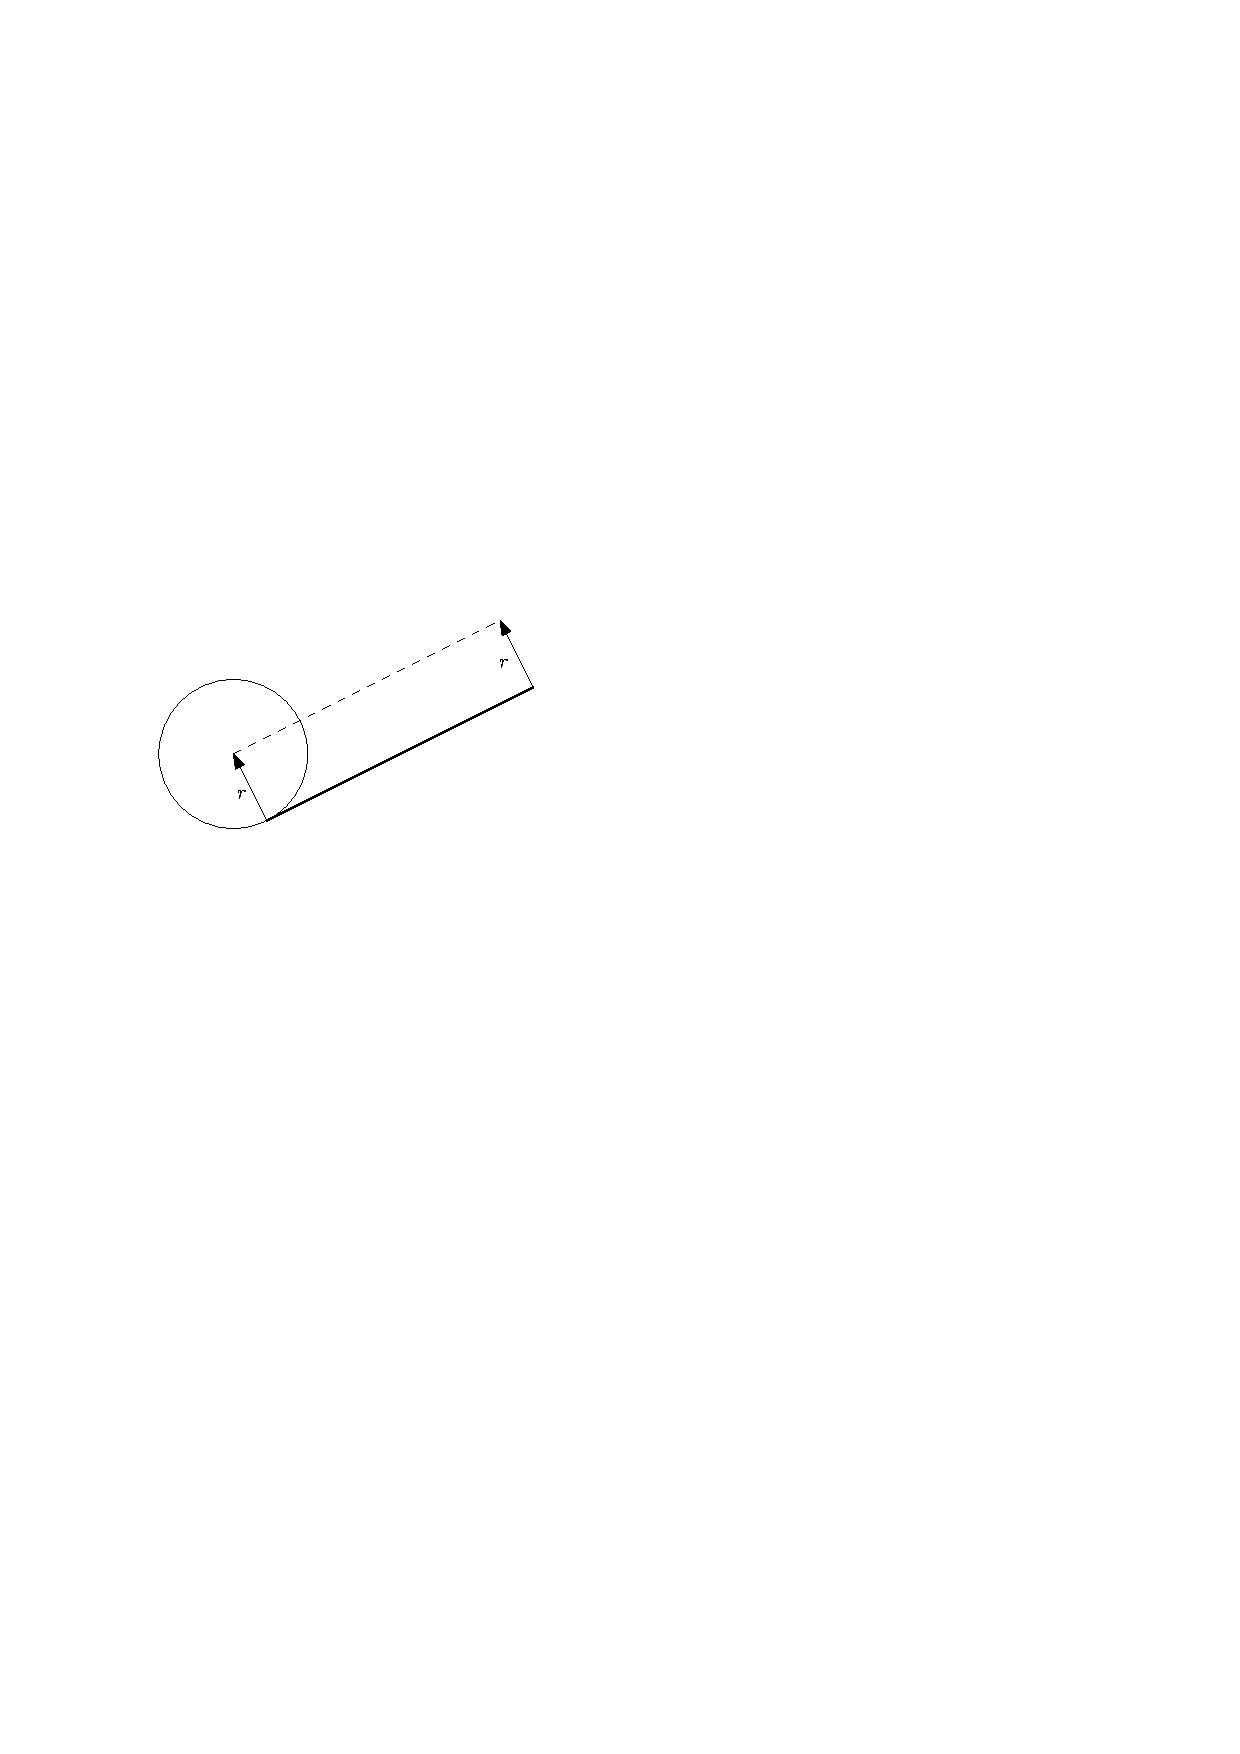
\includegraphics[width=\textwidth]{img/korekce-lin-jedn.pdf}
						\caption{Korekce na úsečce}
					\end{subfigure}
					~~~~~~~~~~~~~~~~~~~
					\begin{subfigure}[b]{0.25\textwidth}
						\centering
						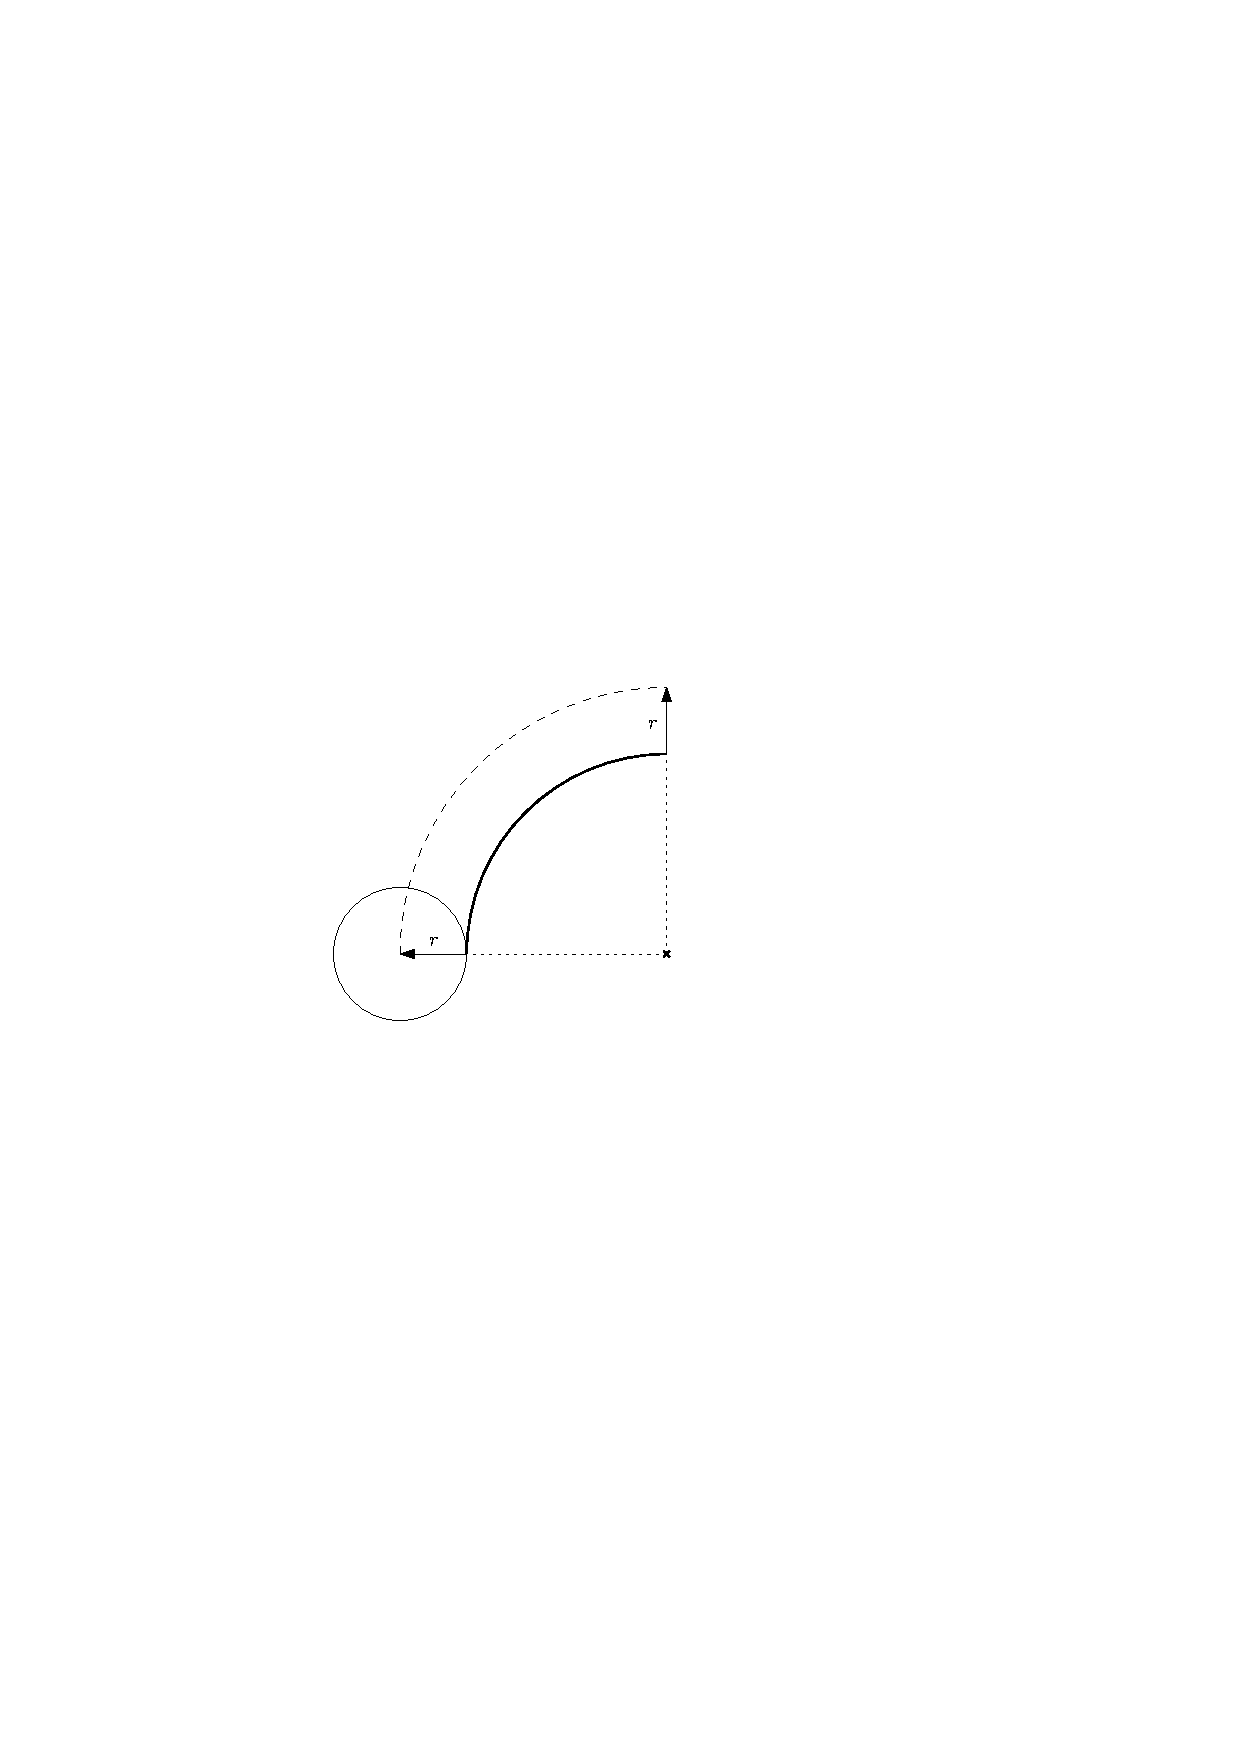
\includegraphics[width=\textwidth]{img/korekce-kruh-jedn.pdf}
						\caption{Korekce na oblouku}
					\end{subfigure}
					\caption{Znázornění základní korekce. Černou čarou je znázorněna naprogramovaná kontura (tedy trasa zadaná G-kódem), přerušovaně pak dopočtená korigovaná trasa.}\label{obr:kor-zak}
			\end{figure}
			Tuto korekci lze provést i na tečně navazujících úsecích se stejnou hodnotou korekce -- jelikož jsou tečné, jejich kolmý vektor v~koncovém bodě prvního a~počátečním bodě druhého úseku je stejný, tudíž zkorigované body splynou a~po korekci dostávám spojitou trasu.
			
			\subsubsection{Korekce pro úseky nenavazující tečně}
			
			Pokud bych na úseky, které na sebe tečně nenavazují použil výše uvedenou korekci, dostal bych nespojitou zkorigovanou trasu. V~tomto případě navázání je nutné rozlišit několik případů. Z~pohledu korekce je nutné hlavně rozlišit, zdali se jedná o vnitřní nebo vnější roh. Z~pohledu výpočtu je ještě nutné rozlišit, mezi jakými druhy úseků korekce nastává. Možné situace jsou znázorněny na obrázcích \ref{obr:kor-netec}.
			
			\begin{figure}[h]
				\centering
					\begin{subfigure}[b]{0.3\textwidth}
						\centering
						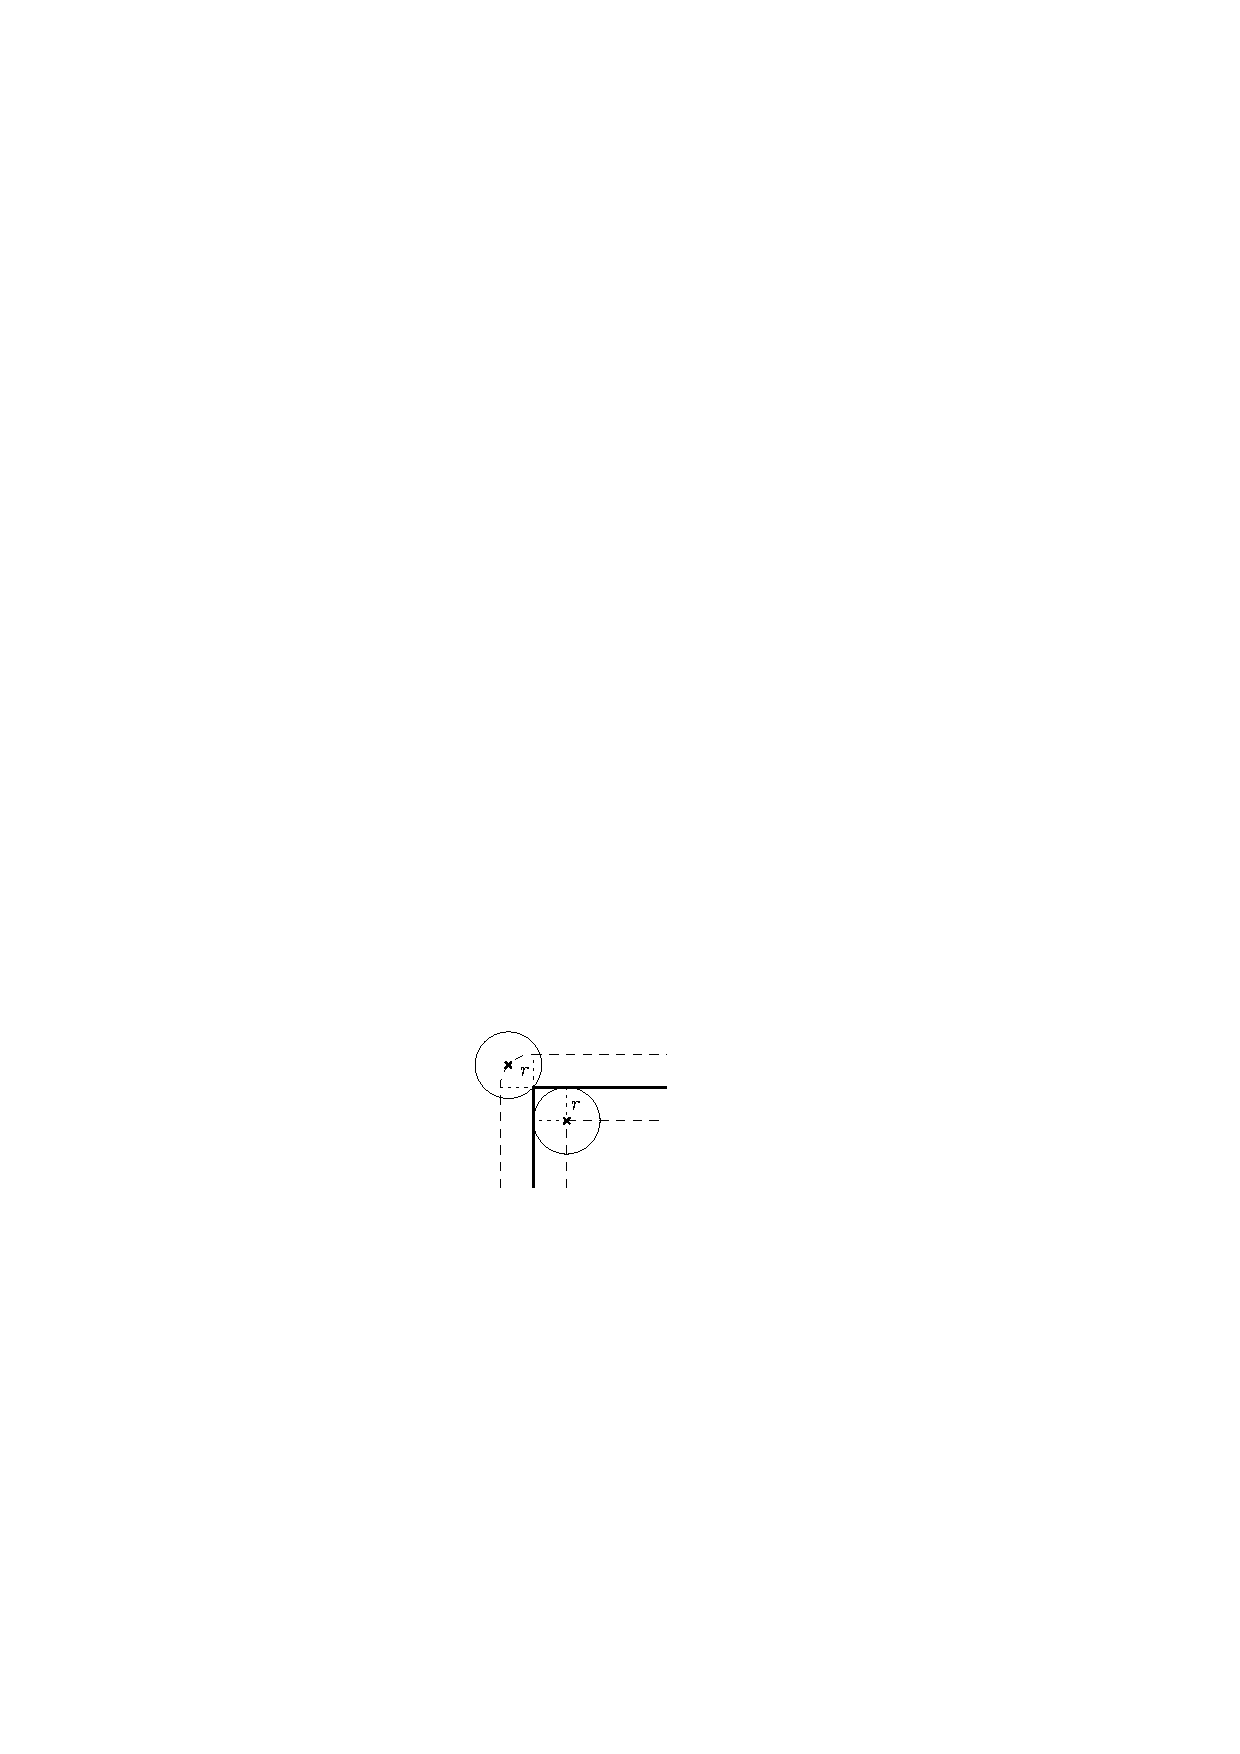
\includegraphics[width=\textwidth]{img/korekce-lin-dva.pdf}
						\caption{Korekce na úsečkách}
					\end{subfigure}
					~
					\begin{subfigure}[b]{0.3\textwidth}
						\centering
						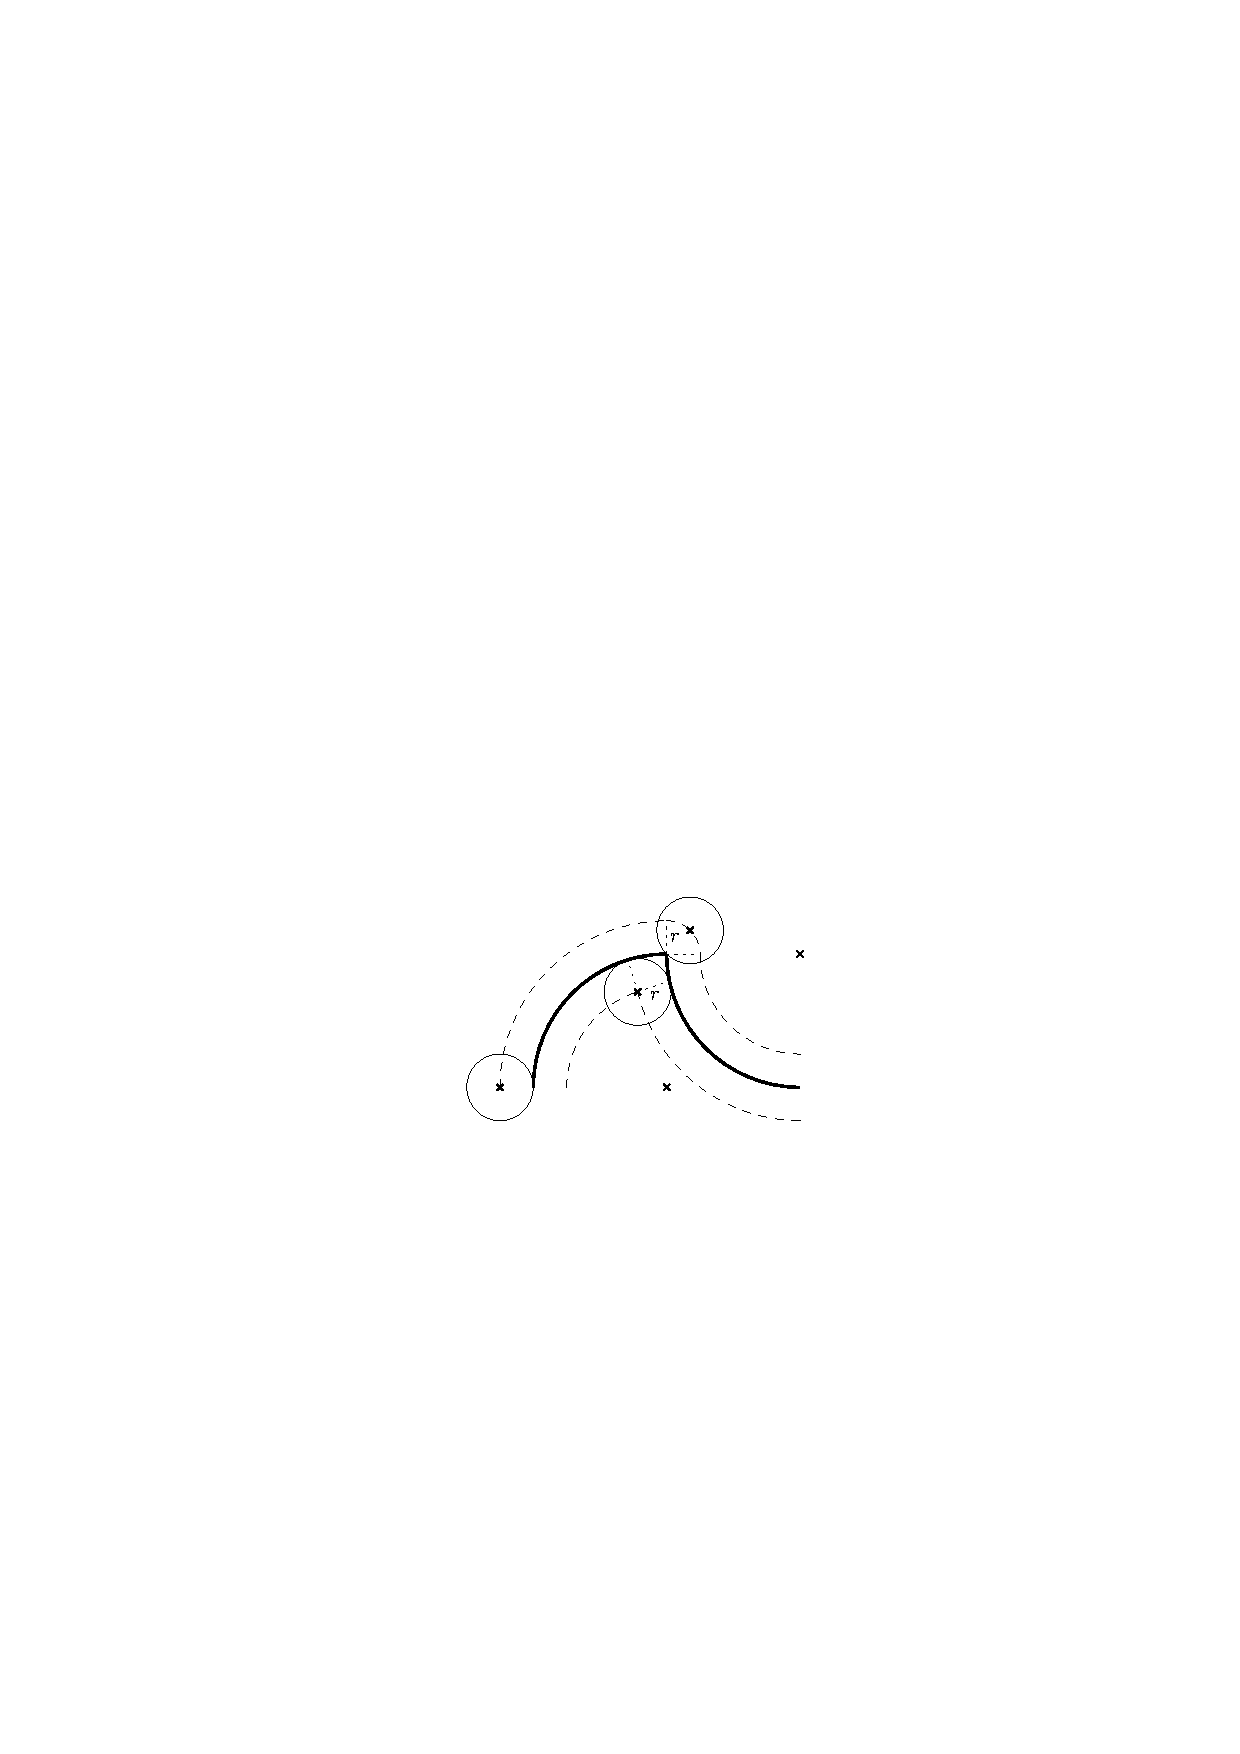
\includegraphics[width=\textwidth]{img/korekce-kruh-dva.pdf}
						\caption{Korekce na obloucích}
					\end{subfigure}
					~
					\begin{subfigure}[b]{0.3\textwidth}
						\centering
						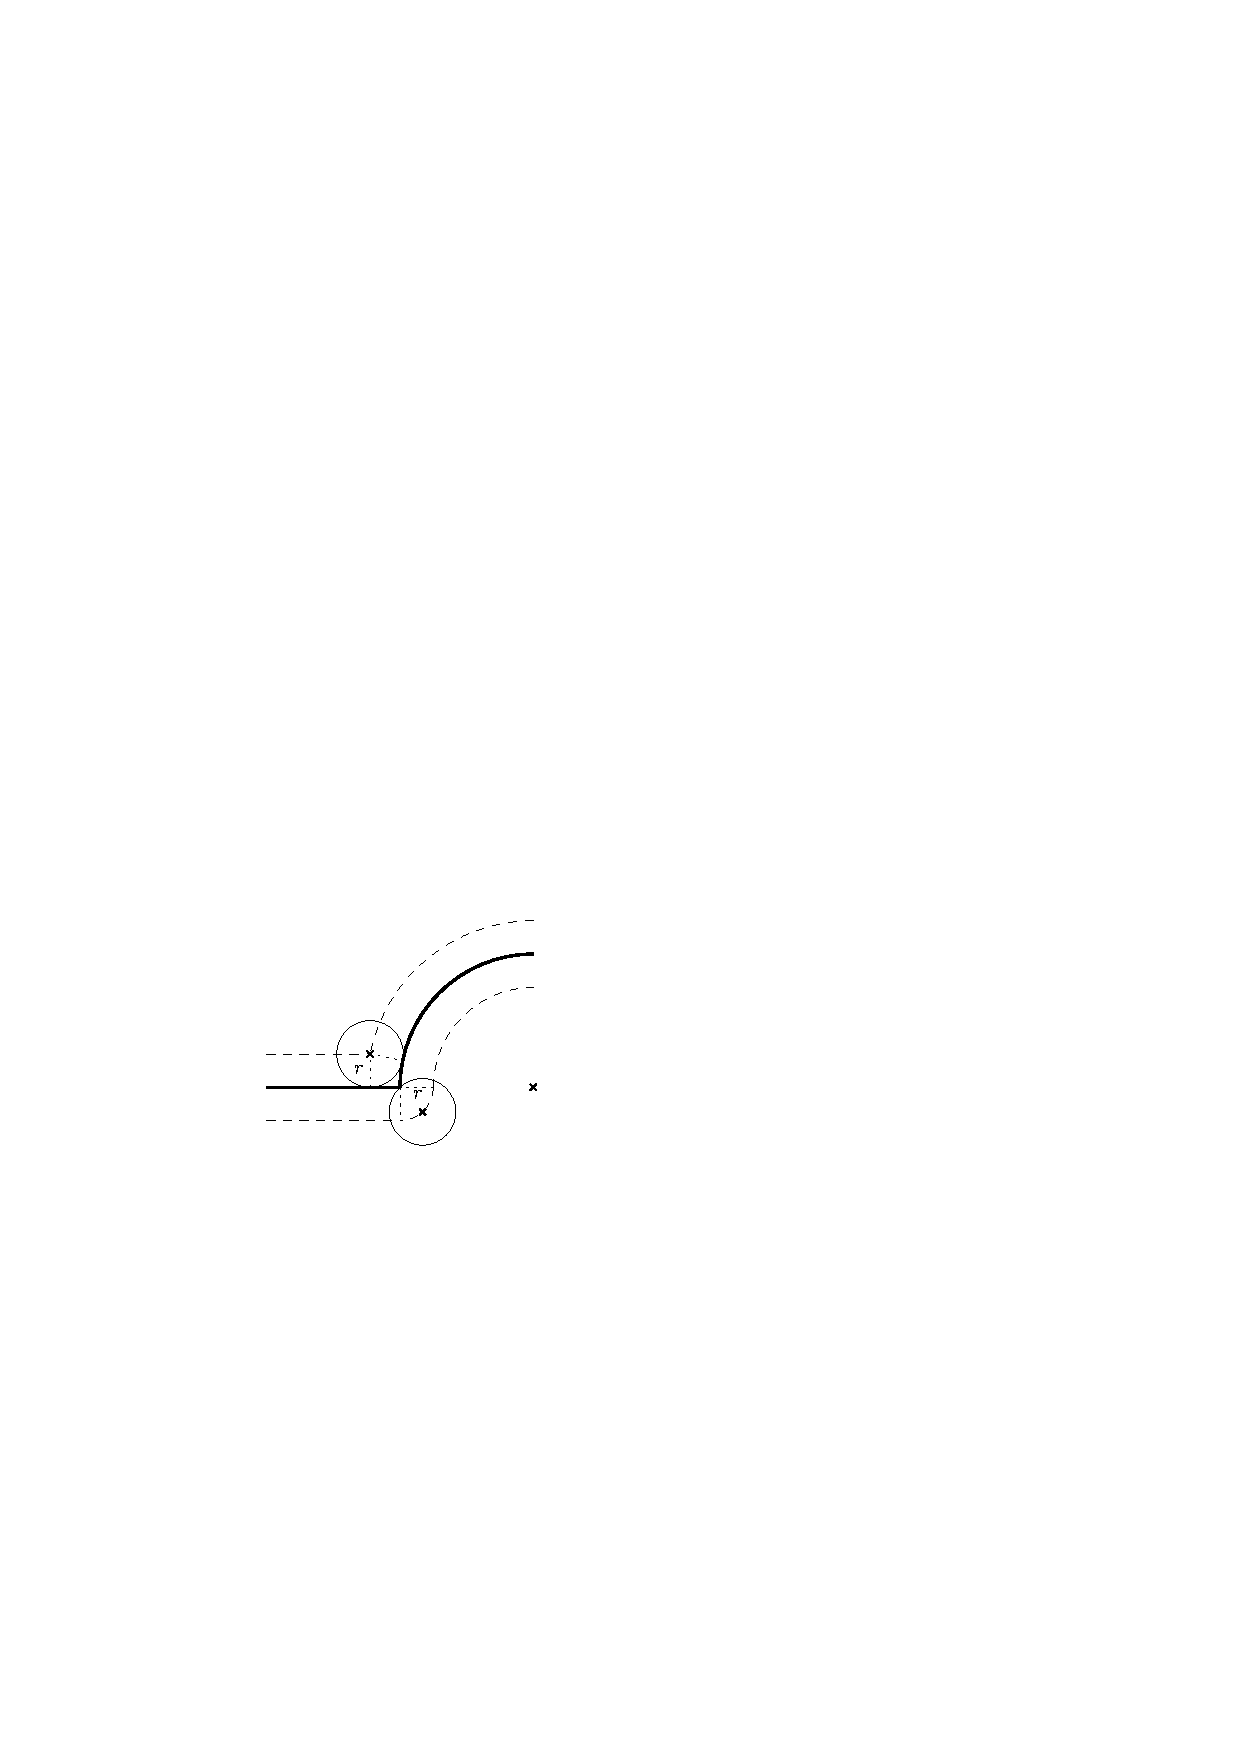
\includegraphics[width=\textwidth]{img/korekce-komb-dva.pdf}
						\caption{Kombinovaná korekce}
					\end{subfigure}
				\caption{Znázornění korekcí na tečně nenavazujících úsecích. Tlustou čarou je zde znázorněna naprogramovaná kontura (původní trasa zadaná G-kódem), přerušovaně pak dopočítaná korekce trasy.}\label{obr:kor-netec}
			\end{figure}
			
			Provedení odsazení vnějšího rohu je relativně jednoduché. Pro zkrácení obráběcího času se neprojíždí plné odsazení, nýbrž se roh opíše obloukem\cite{heid}. Tím je dosaženo zkrácení trasy z~$2r$ na $\frac{\pi}{2}r$. Zároveň se tím však zjednodušuje výpočet korigované trasy. Oba úseky stačí zpracovat stejně jako v~základním případě podle vztahu \ref{rov:odsz} a~mezi koncový odsazený bod prvního úseku a~počáteční odsazený bod druhého úseku vložit oblouk se středem v~koncovém neodsazeném bodu prvního úseku (popř. počátečním neodsazeném bodu druhého úseku, jelikož tyto body jsou totožné). Při obrábění vnějšího rohu nevznikají žádné nepřesnosti.
			
			Pro zpracování vnitřního rohu je třeba nalézt průsečík již zkorigovaných úseků. Jak lze vidět na obrázcích \ref{obr:kor-netec}, vzniká při obrábění vnitřního rohu nepřesnost, kterou nelze nijak korigovat. Lze ji pouze minimalizovat použitím menšího nástroje.
			
			Nejjednodušší situace nastává u dvou netečně navazujících úseček. Průsečík zde hledám tak, že si parametricky vyjádřím zkorigované úsečky (k~parametrickému vyjádření původní trasy přičtu $k\cdot\vec{n}$). Tato soustava vypadá následovně:
			\begin{equation}
				\begin{cases}
				\vec{P}=\vec{A}+p\cdot\vec{u}+k\cdot\vec{n} \\
				\vec{P}=\vec{B}+q\cdot\vec{v}+k\cdot\vec{m},
				\end{cases}
			\end{equation}
			kde $p$ a~$q$ jsou parametry, $u$ a~$v$ směrové vektory, $n$ a~$m$ přislušné normálové vektory a~$k$ je hodnota korekce nástroje.
			
			Porovnáním těchto dvou rovnic a~následným vyřešením získám hodnotu parametru, ze kterého lze jednoduše dopočítat průsečík, což je koncový a~počáteční bod příslušných zkorigovaných úseků.
			\begin{equation}
				p=\frac{-A_1+A_2+B_1-B_2+m_1-m_2-n_1+n_2}{u_1-u_2}	
			\end{equation}
			
			Obdobně lze naléz i průsečík dvou oblouků -- pro zjednodušení výpočtu však všechny útvary posunu tak, aby střed jedné z~kružnici ležel v~bodě $[0;0]$ a~po provedení výpočtu výsledek posunu opačným směrem (zpět). Tímto posunem se mi výrazně zjednodušší výpočet, jelikož dostanu jednoduší středovou rovnici jedné z~kružnic:
			\begin{equation}
				\begin{cases}
				x^2+y^2=r_1^2 \text{~~~~~~~~--~rovnice zjednodušená posunem}\\
				(x-m)^2+(y-n)^2=r_2^2, 
				\end{cases}
			\end{equation}
			kde $x$ a~$y$ jsou souřadnice hledaného průsečíku $P[x;y]$, $m$ a~$n$ jsou  souřadnice středu druhé kružnice $S[m;n]$, $r_1$ a~$r_2$ jsou zkorigované poloměry odsazených kružnic (k~poloměru původních oblouků zadaných G-kódem je přičtena korekce $k$).
			
			Řešením této soustavy je tento relativně složitý výraz:
			\begin{equation}
				P[x;y]\begin{cases}
					x = \frac{m^3+m\left(n^2+r_1^2-r_2^2\right)\pm\sqrt{n^2\left(-\left(m^2+n^2-r_1^2\right)^2+2r_2^2\left(m^2+n^2+r_1^2\right)-r_2^4\right)}}{2\left(m^2+n^2\right)}\\
					y = \frac{n^4+n^2\left(m^2+r_1^2-r_2^2\right)\mp m \sqrt{n^2\left(-\left(m^2+n^2-r_1^2\right)^2+2r_2^2\left(m^2+n^2+r_1^2\right)-r_2^4\right)}}{2n\left(m^2+n^2\right)}
				\end{cases}
			\end{equation}
			Existují dva průsečíky těchto kružnic, bohužel se mi nepodařilo zjistit, jak předem rozlišit, který průsečík je ten mnou hledaný. V~mém kódu tedy počítám oba dva a~za správný považuji ten, který leží blíže původnímu napojení nekorigovaných oblouků.
			
			Poslední případ, který může nastat je vnitřní roh mezi obloukem a~úsečkou. Zde opět využiji parametrického vyjádření úsečky, které následně dosadím do obecné rovnice kružnice. Opět v~zájmu zjednodušení byl proveden posun tétou soustavy tak, aby střed oblouku ležel v~bodě $[0;0]$.
			\begin{equation}
				\begin{cases}
				\vec{P}=\vec{A}+p\cdot\vec{u}+k\cdot\vec{n} \\
				x^2+y^2=r^2
				\end{cases}
			\end{equation}
			Pro zjednodušení výrazu sloučím v~rovnici přímky konstantní výrazy v~konstantu $\vec{k}$:
			\begin{equation}
			\vec{A}+k\cdot\vec{n}=\vec{k}	
			\end{equation}
			Po rozdělení rovnice přímky na dvě (pro $x$-ové a~$y$-ové souřadnice) a~jejich dosazení do rovnice kružnice, dostávám následující vztah pro parametr $p$:
			\begin{equation}
				p=\frac{\pm k_1u_1\pm k_2u_2\mp\sqrt{u_1^2(r^2-k_2^2)+2k_1k_2u_1u_2+u_2^2(r^2-k_1^2)}}{u_1^2+u_2^2},
			\end{equation}
			z~něhož snadno dopočítám oba průsečíky. Stejně jako v~předchozím případě, i~zde jsem nepřišel na způsob, jak předem určit, který z~parametrů je mnou hledaný. Proto opět počítám oba dva a~vybírám bod, který je blíže průsečíku původních nekorigovaných úseků.
			
		\subsubsection{Korekce pro úseky se změnou její hodnoty}
			To, jak se má korekce chovat, pokud je nastavena, je relativně logické. Standard však nedefinuje, jak se má systém zachovat po spuštění korekce. Rozhodl jsem se respektovat chování systémů LinuxCNC\cite{emckor} a~Heidenhein\cite{heid}. Tyto systémy považují první pohyb po aplikování korekce za \uv{lead-in}\footnote{termín používaný v~dokumentaci LinuxuCNC\cite{emckor}, nenašel jsem adekvátní překlad, proto v~textu používám anglický výraz}. Tento pohyb by neměl být určen k~obrábění a~jeho cílem je aplikovat korekci -- na svém konci by měl být nástroj již ve správném odsazení od~původní trasy. Jako vzor chování stroje během lead-in pohybu jsem si vzal chování systému LinuxCNC (popsáno v~\cite{emckor}). Toto chování se však ukázalo v~jednom případě jako nevhodné (viz dále).
			
			Výše uvedené systémy (LinuxCNC, Heidenhein, Sinumerik), akceptují jako lead-in pohyb pouze lineární pohyb (funkci G01), avšak  já jsem se rozhodl do mého systému zaimplementovat i podporu pro obloukový lead-in pohyb (funkce G02, G03).
			
			Celkem tedy mohou nastat čtyři případy: lead-in pohyb je lineární a~navazuje na vnitřní roh; lead-in pohyb je lineární a~navazuje na vnější roh; lead-in pohyb je obloukový a~korekce se zmenšuje; lead-in pohyb je obloukový a~korekce se zvětšuje.
			
			Nejjedodušším případem je lineární lead-in pohyb navazující na vnitřní roh. Zde jsem se také po konzultaci na diskusním fóru C-N-C.cz\footnote{\url{http://www.c-n-c.cz/viewtopic.php?f=47\&t=9669}} rozešel s~implementací LinuxuCNC. Implementace systémem LinuxCNC je znázorněna na nákresu \ref{nak:EMCk}. Logikou tohoto systému je, že nástroj nesmí odebrat materiál mimo zadanou konturu, proto raději zanechá neobrobenou část na kontuře\cite{emckor}.
			
			Po konzultaci na diskusním fóru jsem si stanovil pro můj systém stejnou prioritu jako systém Heidenheim\cite{heid} -- systém musí, co nejpřesněji obrobit zadanou konturu. Na nákresech \ref{nak:leadin1} je znázorněno chování mého systému. Na nákresu b si lze povšimnout, že systém porušuje konturu lead-in pohybu. Jak jsem však již dříve zmínil, lead-in pohyb by neměl obrábět. Proto porušení jeho kontury nevadí. Ve správně napsaném programu by v~prostoru lead-in pohybu neměl být žádný materiál.
			
			Z této úvahy vyplývá, že pro zpracování lineárního lead-in pohybu stačí počáteční bod zpracovat stejně, jako by se jednalo o~klasickou konturu, a~jeho koncový bod má souřadnice:
			\begin{equation}
			\vec{P} = \vec{B}+k\cdot\vec{n},
			\end{equation}
			kde $\vec{B}$ je počáteční bod navazujícího úseku, $\vec{n}$ normálový vektor navazujícího úseku a~$k$ je hodnota korekce.
			
			\begin{figure}[h]
				\centering
				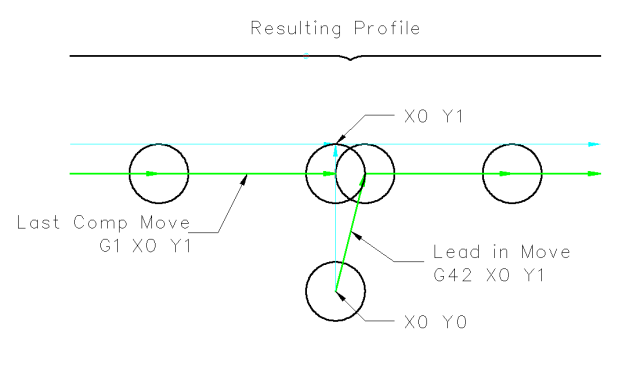
\includegraphics[width=0.6\textwidth]{img/comp02.png}
				\caption{Implementace chování lineárního lead-in pohybu v~systému LinuxCNC. Převzato z~\url{http://www.linuxcnc.org/docs/2.4/html/comp02.png}}\label{nak:EMCk}	
			\end{figure}
			
			\begin{figure}[h]
				\centering
					\begin{subfigure}[b]{0.42\textwidth}
						\centering
						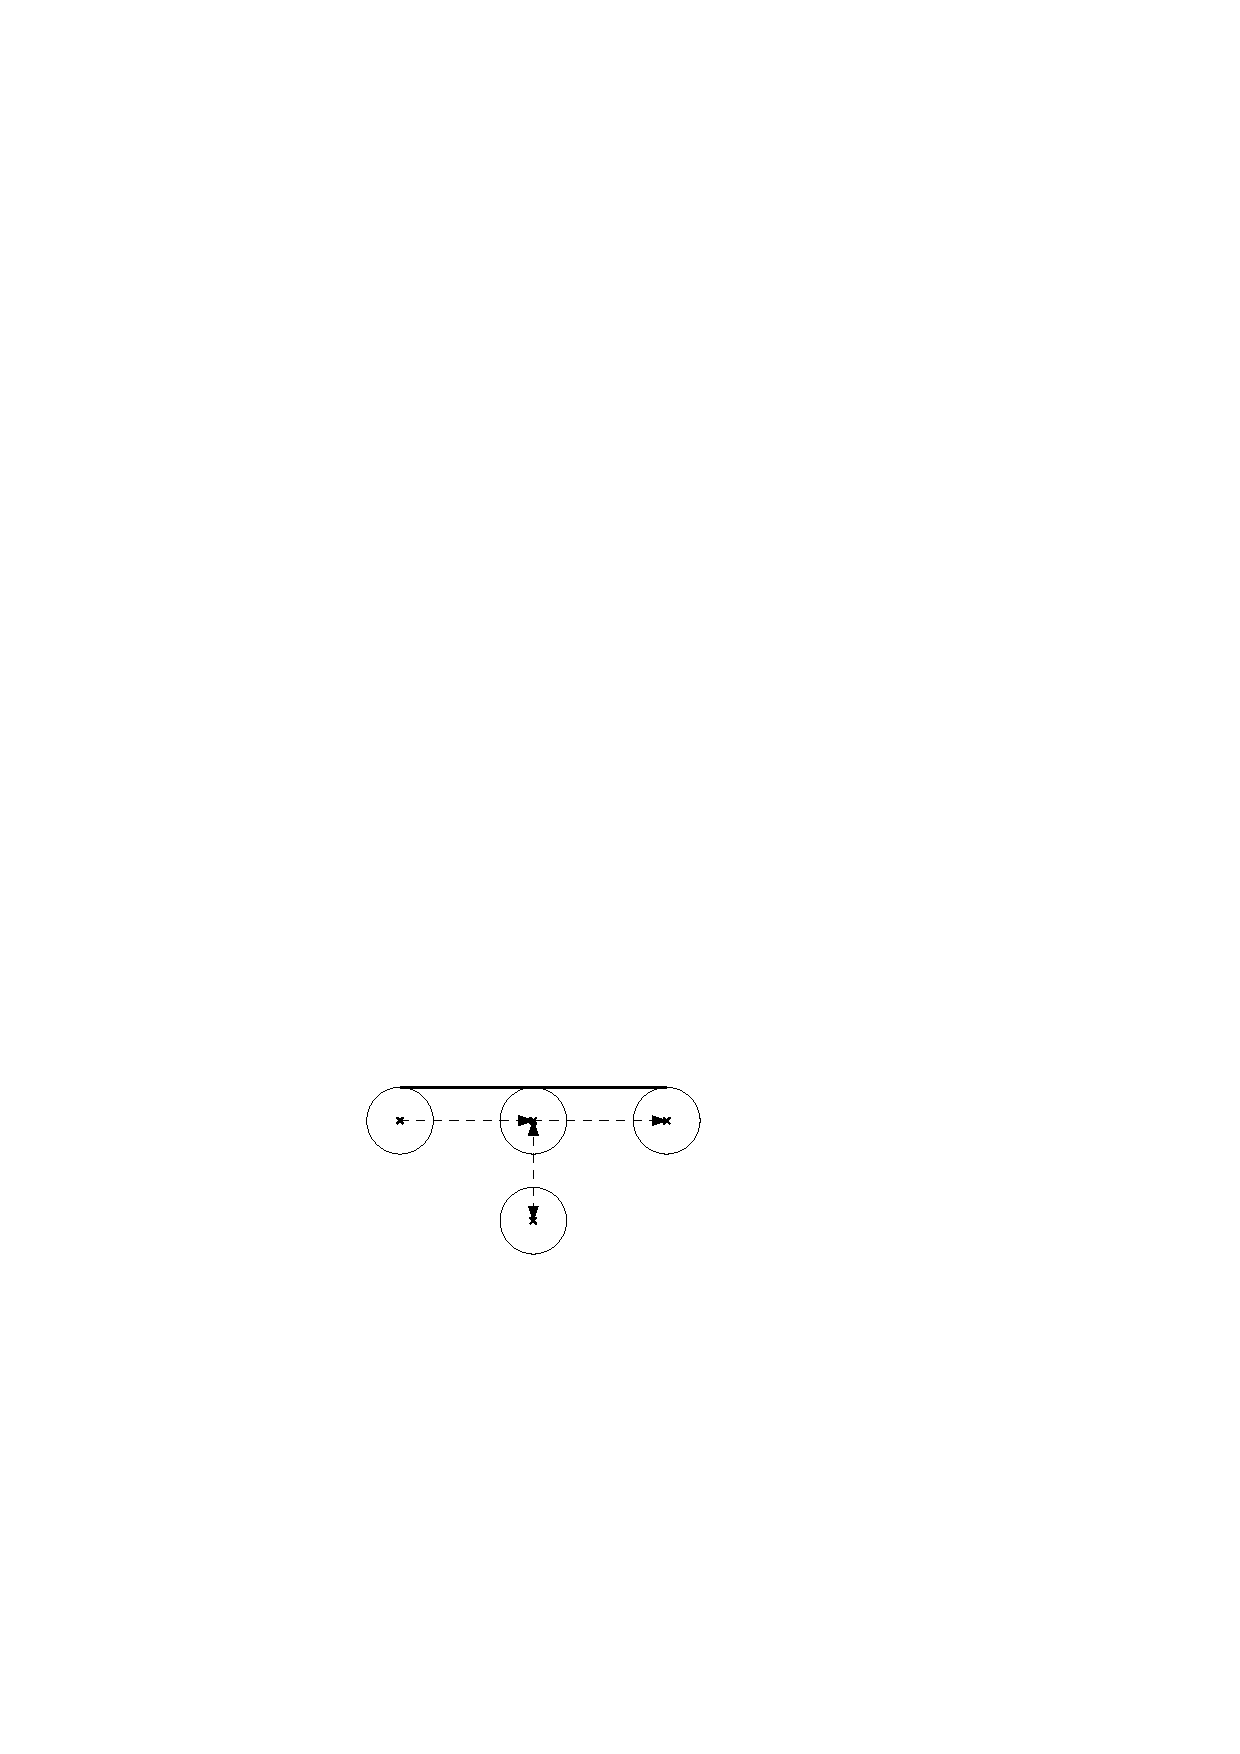
\includegraphics[width=\textwidth]{img/korekce-leadin1.pdf}
						\caption{Mé řešení situace z~dokumentace LinuxCNC}
					\end{subfigure}
					~~~
					\begin{subfigure}[b]{0.3\textwidth}
						\centering
						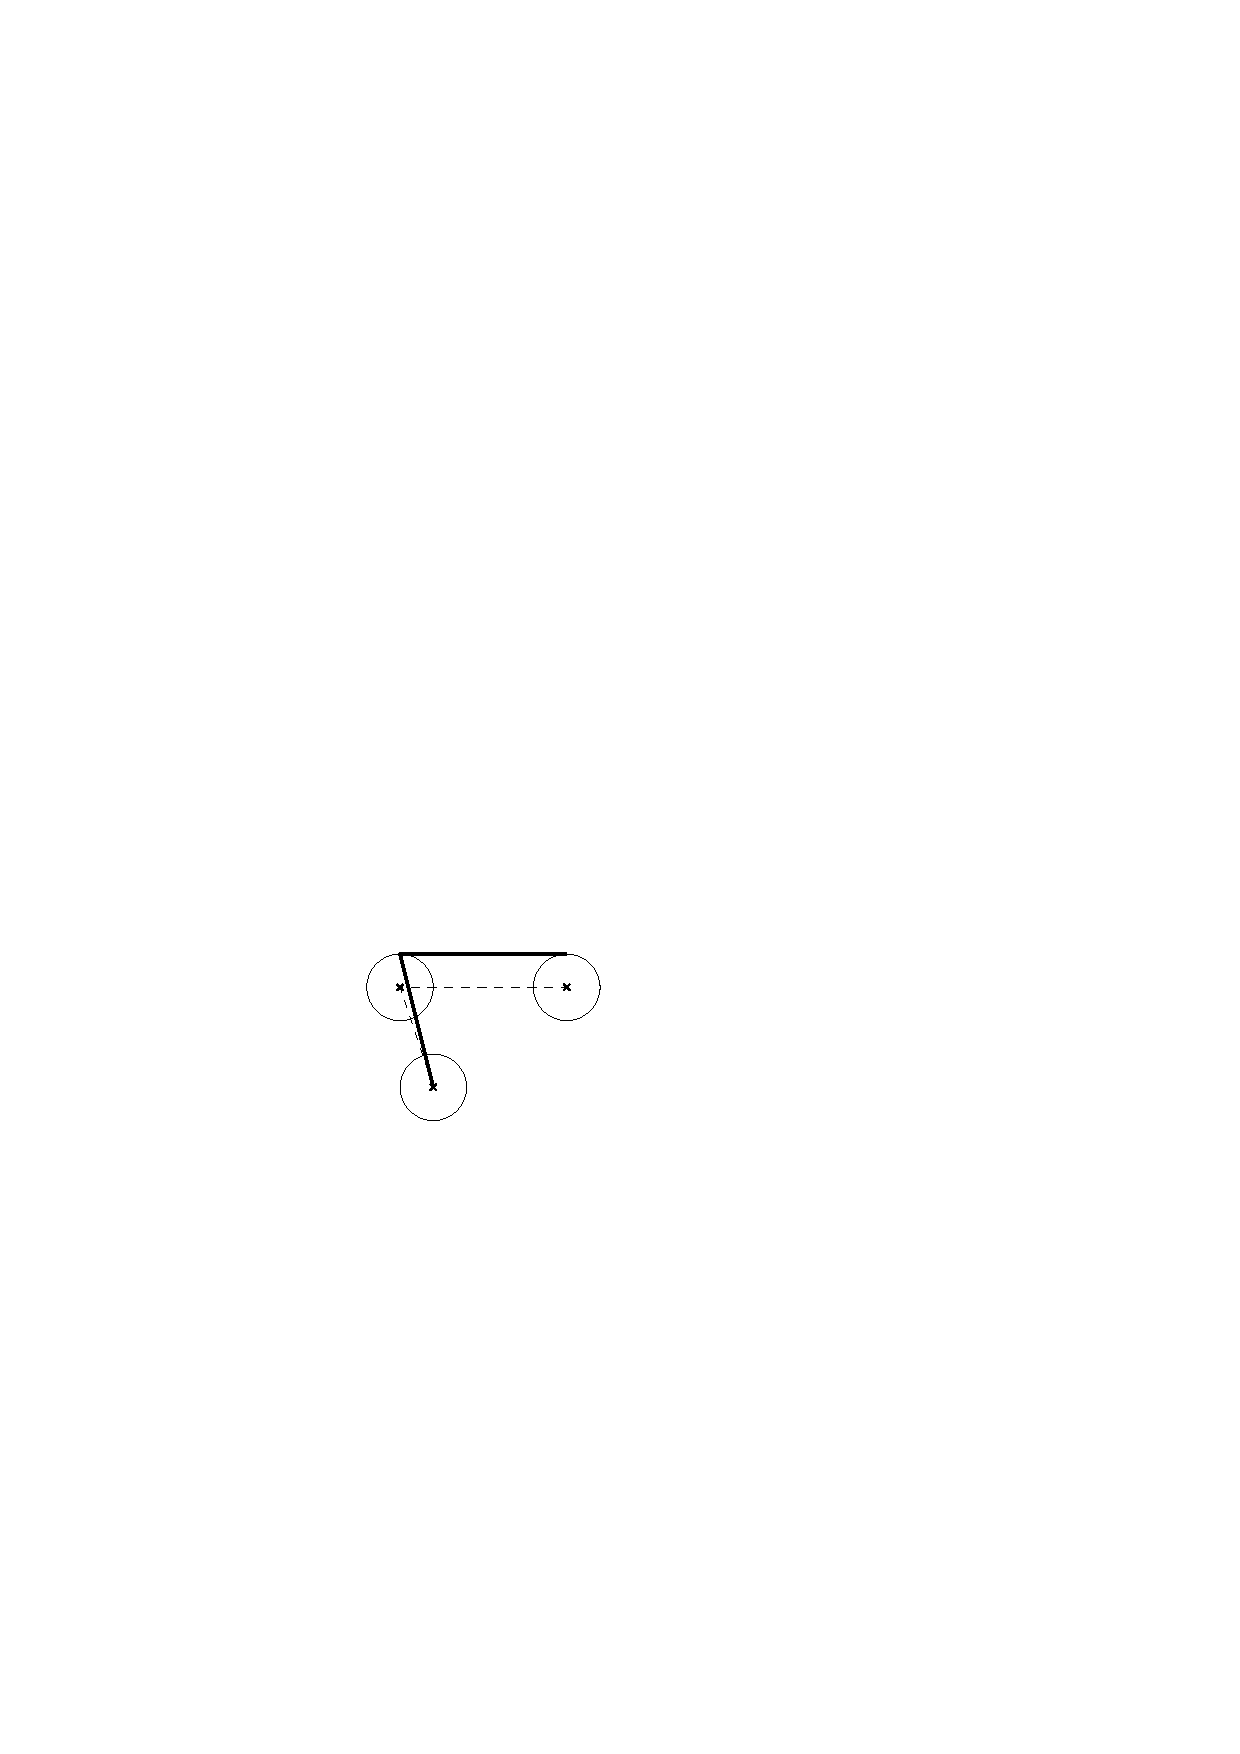
\includegraphics[width=\textwidth]{img/korekce-leadin2.pdf}
						\caption{Obecný případ}
					\end{subfigure}
				\caption{Implementace lineárního lead-in pohybu v~mém systému. Tlustá čára znázorňuje trasu zadanou G-kódem, přerušovaná pak dopočtenou korekci.}\label{nak:leadin1}
			\end{figure}
			
			Pokud lineární lead-in pohyb navazuje na vnější roh, je situace obdobná jako v~případě klasického korigovaného pohybu -- vnější roh je obroben vloženým obloukem, který jej opisuje. Pokud bych však na počátku a~na konci lead-in pohybu použil jinou hodnotu korekce, nenavazoval by tento oblouk tečně, tudíž by těsně před ním musel stroj zabrzdit. Ideálně by měl oblouk navazovat tečně, jak znázorňuje obrázek \ref{nak:leadin3}.
			
			Výpočet pozice bodu C jsem v~tomto případě realizoval skrz vektor odsazení $\vec{o}$. Mé řešení vychází z~pravoúhlého trojúhelníku ABC. Pokud budu uvažovat vektor mezi body A a~B jako~$\vec{u}$, mohu úhel $\alpha$ vyjádřit následovně:
			\begin{equation}
				\vec{u}\cdot\vec{o}=\cos\alpha
			\end{equation}
			Jelikož je délka vektoru $\vec{o}$ rovna korekci $\abs{k}$, tak můžu vyjářit $\cos\alpha$ i pomocí těchto délek. Získám tedy soustavu rovnic:
			\begin{equation}
				\begin{cases}
					\vec{u}\cdot\vec{o} = \frac{\abs{k}}{\abs{\vec{u}}} \\
					\abs{\vec{o}}=\abs{k} \implies o_1^2+o_2^2=k^2
				\end{cases}
			\end{equation}
		Pokud označím $\abs{\vec{u}}=d$, řešením této soustavy je
			\begin{equation}
			\vec{o}
			\begin{cases}
				o_1=\frac{dku_1\pm\sqrt{d^2k^2u_2^2 \left(d^2\left(u_1^2+u_2^2\right)-1\right)}}{d^2\left( u_1^2+u_2^2\right)} \\
				o_2=\frac{dku_2^2\mp u_1\sqrt{d^2k^2u_2^2\left(d^2\left(u_1^2+u_2^2\right)-1\right)}}{d^2u_2(u_1^2+u_2^2)}
			\end{cases}
			\end{equation}
			Tento výraz je použitelný i pro situaci, kdy původní korekce nebyla nulová, či dokonce měla opačný směr. Pouze se jako bod A vezme již jeho zkorigovaná hodnota. Nadále zde zůstává pravoúhlý trojúhelník. U~tohoto výrazu se mi podařilo určit znaménko ve vzorci pro určení požadovaného řešení. Pokud se nová korekce nachází na stejné straně od~kontury jako předcházející, je ve výrazu pro $o_1$ plus a~ve výrazu $o_2$ mínus. Pokud se původní korekce nacházela na opačné straně od~kontury, jsou znaménka přesně opačná.
		
			\begin{figure}[h]
				\centering
				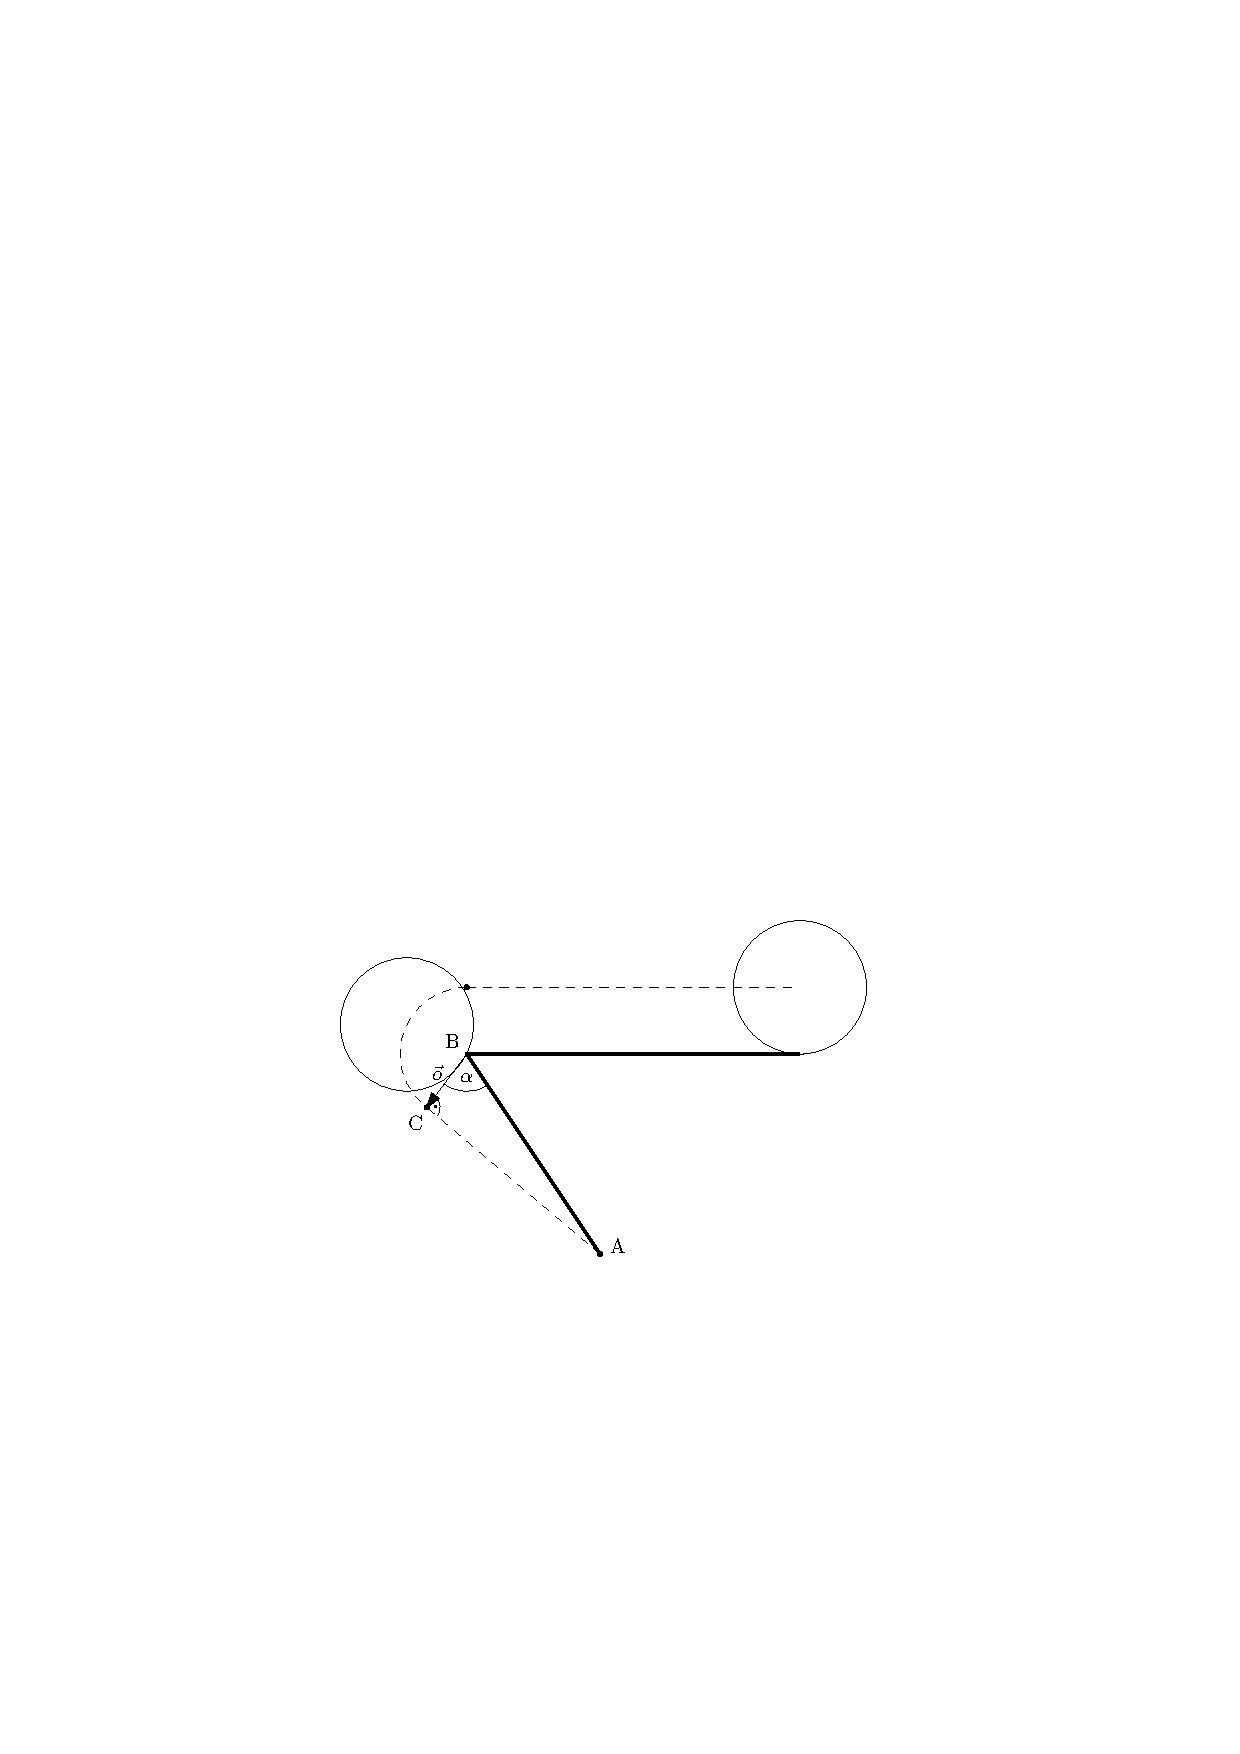
\includegraphics[width=0.5\textwidth]{img/korekce-leadin3.pdf}
				\caption{Znázornění implementace lead-in pohybu, který navazuje na vnější roh.}\label{nak:leadin3}	
			\end{figure}
			
			Jak jsem zmínil v~úvodu této sekce, rozhodl jsem se do mého systému zaimplementovat podporu pro obloukový lead-in pohyb. Jsou dvě možnosti korekce -- výsledkem první je oblouk o menším poloměru, výsledkem druhé je oblouk o větším poloměru. Obě situace znázorňují nákresy~\ref{nak:leadinobl}.
			
			Při korekci na oblouk o větším poloměru přidám do trasy úsečku délky $k$ ve směru tečném k~počátečnímu bodu oblouku. Následně za tento lineární úsek přidám oblouk o původním poloměru a~úhlové délce 90~$^\circ$. V~jeho koncovém bodě se již nástroj dostává do zkorigované pozice a~následuje oblouk již o zkorigovaném poloměru.
			
			Při korekci na oblouk o menším poloměru je postup opačný -- pohyb začíná obloukem se~zkorigovaným poloměrem a~úhlové délce 90~$^\circ$. Za něj vkládám lineární úsek o délce $k$. V~tomto bodě se již nástroj nachází ve~zkorigované pozici a~následuje zkorigovaný původní oblouk kontury.
			
			Z~mnou použitého řešení, jak implementovat oblouk jako lead-in pohyb, vyplývá jedno omezení -- jako lead-in pohyb nelze použít oblouk, který má úhlovou délku kratší než 90~$^\circ$.
			
			
			Na obrázku \ref{nak:korvys} si lze prohlédnout výstup již implementované korekce průměru v~mém systému. Korekce je znázorněna bílou čarou. Jedná se o ukázkový příklad, kdy byly do jednoduchého programu v G-kódu na náhodná místa přidány funkce G40, G1 a~G42.
			
			\begin{figure}[h!]
				\centering
					\begin{subfigure}[b]{0.40\textwidth}
						\centering
						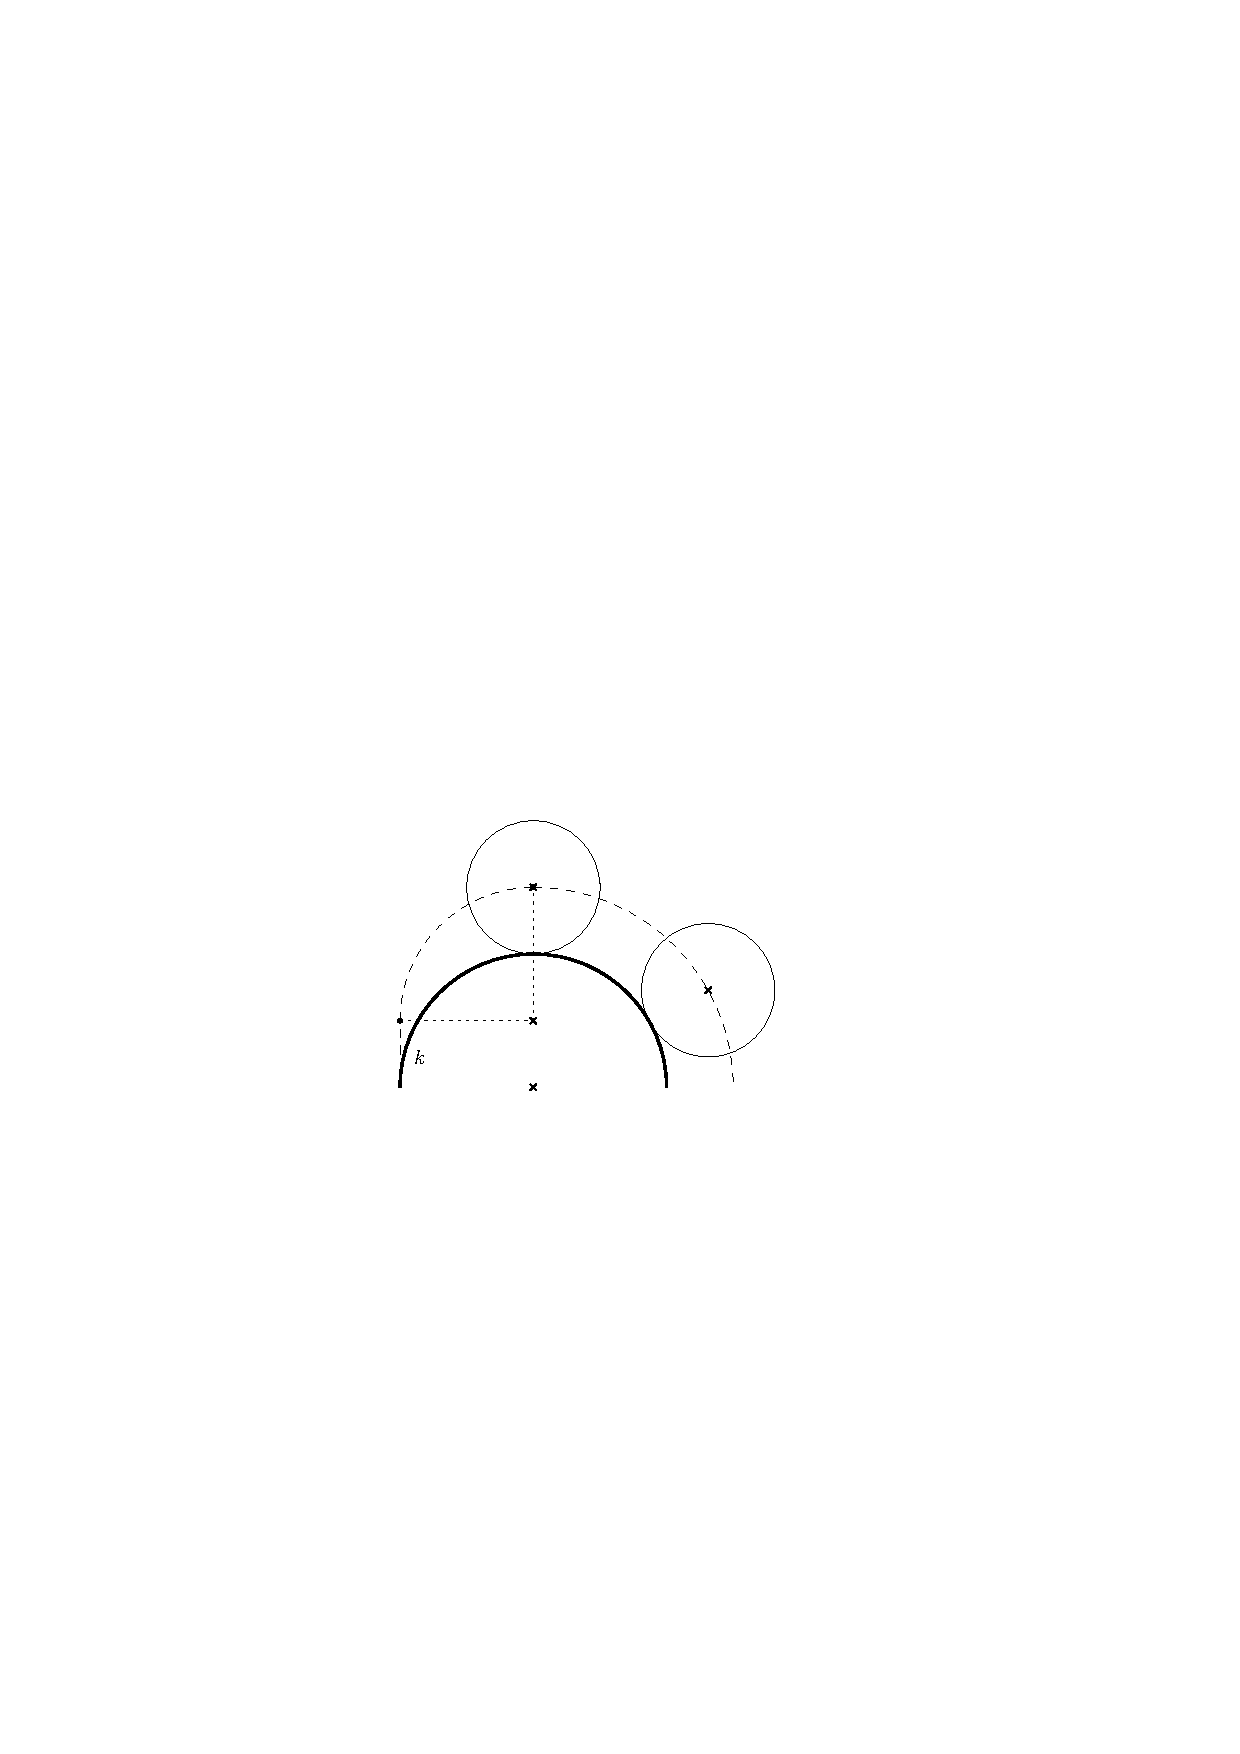
\includegraphics[width=\textwidth]{img/korekce-leadin4.pdf}
						\caption{Korekce na větší poloměr}
					\end{subfigure}
					~~~
					\begin{subfigure}[b]{0.40\textwidth}
						\centering
						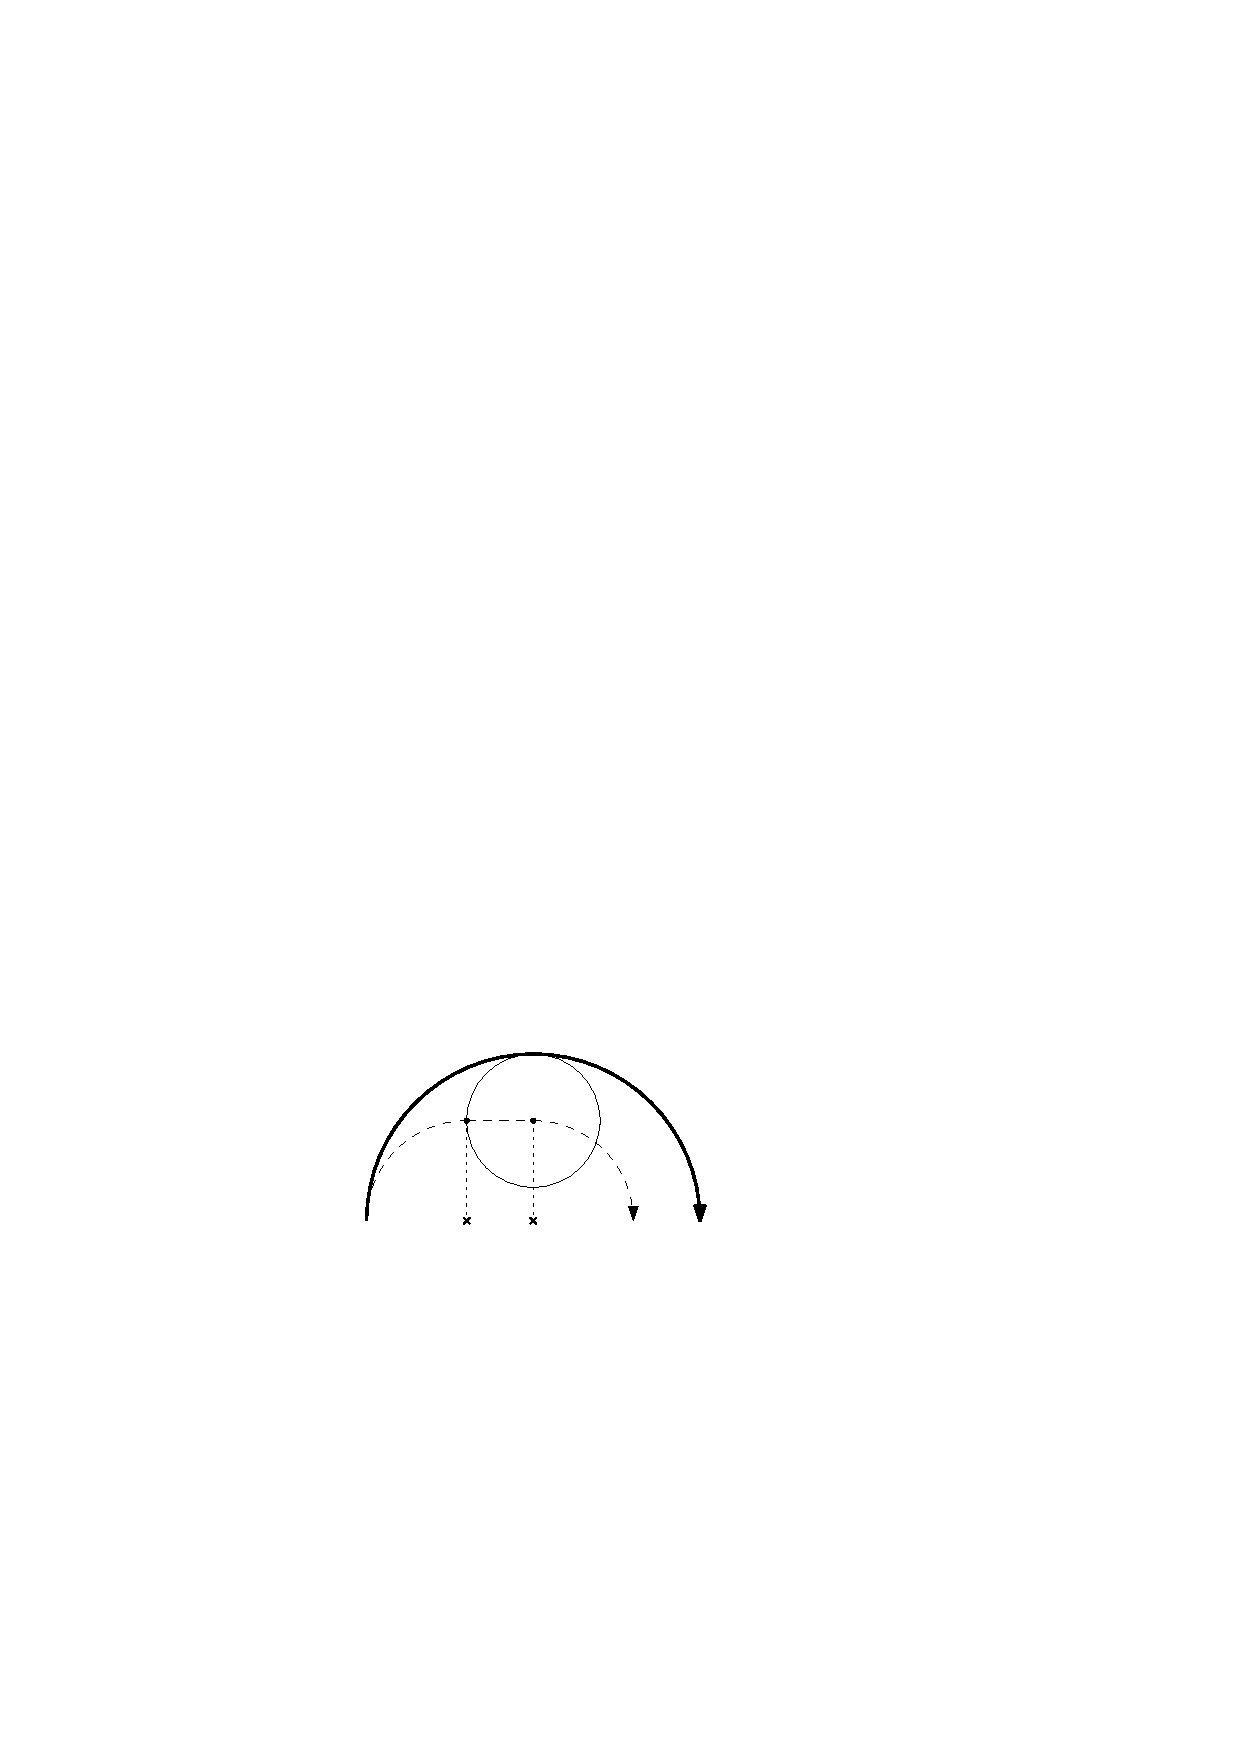
\includegraphics[width=\textwidth]{img/korekce-leadin5.pdf}
						\caption{Korekce na menší poloměr}
					\end{subfigure}
				\caption{Znázornění implementace obloukového lead-in pohybu}\label{nak:leadinobl}
			\end{figure}
			
		\begin{figure}[h!]
			\centering
			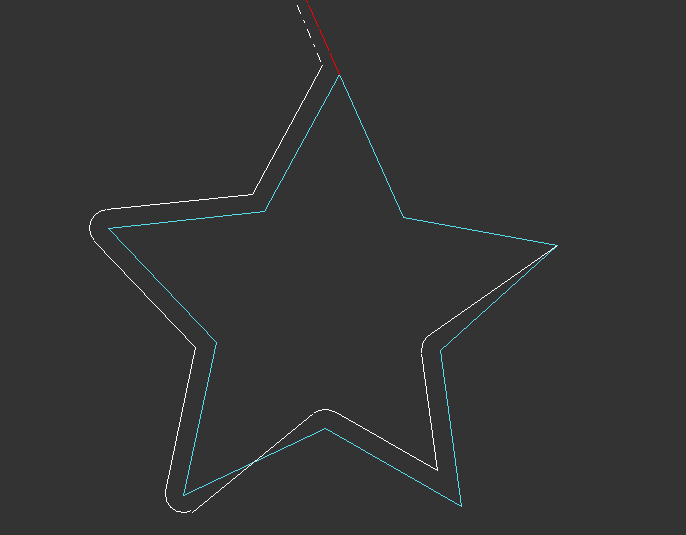
\includegraphics[width=0.7\textwidth]{img/korekce.png}
			\caption{Ukázka zpracování korekce průměru nástroje mým systémem. Na počátku kontury je nastavena korekce doprava ve směru obrábění, na třetím vrcholu hvězdy, je změněna korekce na opačnou (doleva).  Za čtvrtým vrcholem je korekce vypnuta.}\label{nak:korvys}	
		\end{figure}
			
		\subsection{Korekce délky}
		Oproti korekci poloměru nástroje je implementace korekce délky nástroje jednoduchou záležitostí. Jedná se totiž pouze o korekci ve směru jedné osy (Z), narozdíl od~dvou os (X a~Y) v~případě korekce poloměru nástroje.
		
		Počáteční bod každého úseku je nutno zkorigovat o korekci nastavenou pro úsek předcházející a~koncový bod každého úseku je nutno zkorigovat korekcí nastavenou pro aktuálně zpracovávaný úsek.
		
		Zde je nutno podotknout, že tato korekce zatím nebyla v~mém systému plně implementována a~může způsobovat chyby. Na vině je implementace kruhové interpolace, která není v~souladu se~standardem G-kódu (viz kapitola \ref{kap:oblinter}). Pokud by nastala změna délkové korekce na kruhovém oblouku, měl by počáteční a~koncový bod jiné Z-ové souřadnice. Dle standardu by se tato změna měla interpolovat po šroubovici, avšak můj systém se pokusí nalézt kruhový oblouk v~obecné rovině, který tomuto zadání vyhovuje.
		
		
	\section{Výpočet rychlosti}\label{kap:rychlost}
	Poslední činností, kterou vykonává třída {\tt GCodeInterpreter} před tím, než vytvoří seznam příkazů pro interpolátor, je dopočtení rychlostí pro každý úsek.
	
	Rychlost na každém úseku je charakterizována počáteční, cílovou a~brzdnou rychlostí a~také maximálním zrychlením pro rozjezd a~brzďění. Na základě těchto údajů je schopen interpolátor provést pohyb. {\tt GCodeInterpreter} na základě posuvu v~G-kódu, maximálního zrychlení a~ryvu zadaného v~konfiguračním souboru a~tvaru úseku určuje vhodnou rychlost.
	
	Výpočet rychlosti probíhá pro každý úsek samostatně. Pro vypočtení rychlosti celé trasy tedy procházím každý prvek trasy od~konce po začátek. Při provádění výpočtu rychlosti od~konce je totiž menší šance na vznik cyklické závislosti -- může se stát, že vypočtená počáteční rychlost je pro daný prvek příliš velká, a~musím se proto tedy vrátit na $n$ předcházejících prvků a~ty znovu spočítat. Při procházení trasy od~konce však tato situace nastává pouze zřídka, např. při seskupení krátkých oblouků o malém poloměru za sebou. Výpočet rychlosti daného prvku má na starosti metoda {\tt PathPart::ComputeSpeeds}.
	
	V následujícím textu používám pojmy předcházející a~následující úsek. Ačkoliv úseky zpracovávám v~opačném pořadí (od posledního po první), pojmem následující úsek mám na mysli úsek, který následuje během pohybu (tedy pořadí od~prvního po poslední), resp. pojmem předchozí úsek mám na mysli úsek, který předchází během pohybu.
	
	Pro jednotlivé rychlosti platí, že počáteční a~koncová rychlost je menší nebo rovna požadované. Tato podmínka vychází z~logiky, že posuvem je dána maximální možná rychlost na daném úseku, která nesmí být překročena. A jelikož posuv určuje požadovanou rychlost, tak počáteční i koncová rychlost musejí být menší.
	
	Postup výpočtu, který je popsán v~následujících odstavcích je také znázorněn na schématu~\ref{nak:vypocet}.
	
	\begin{figure}[h!]
		\centering
		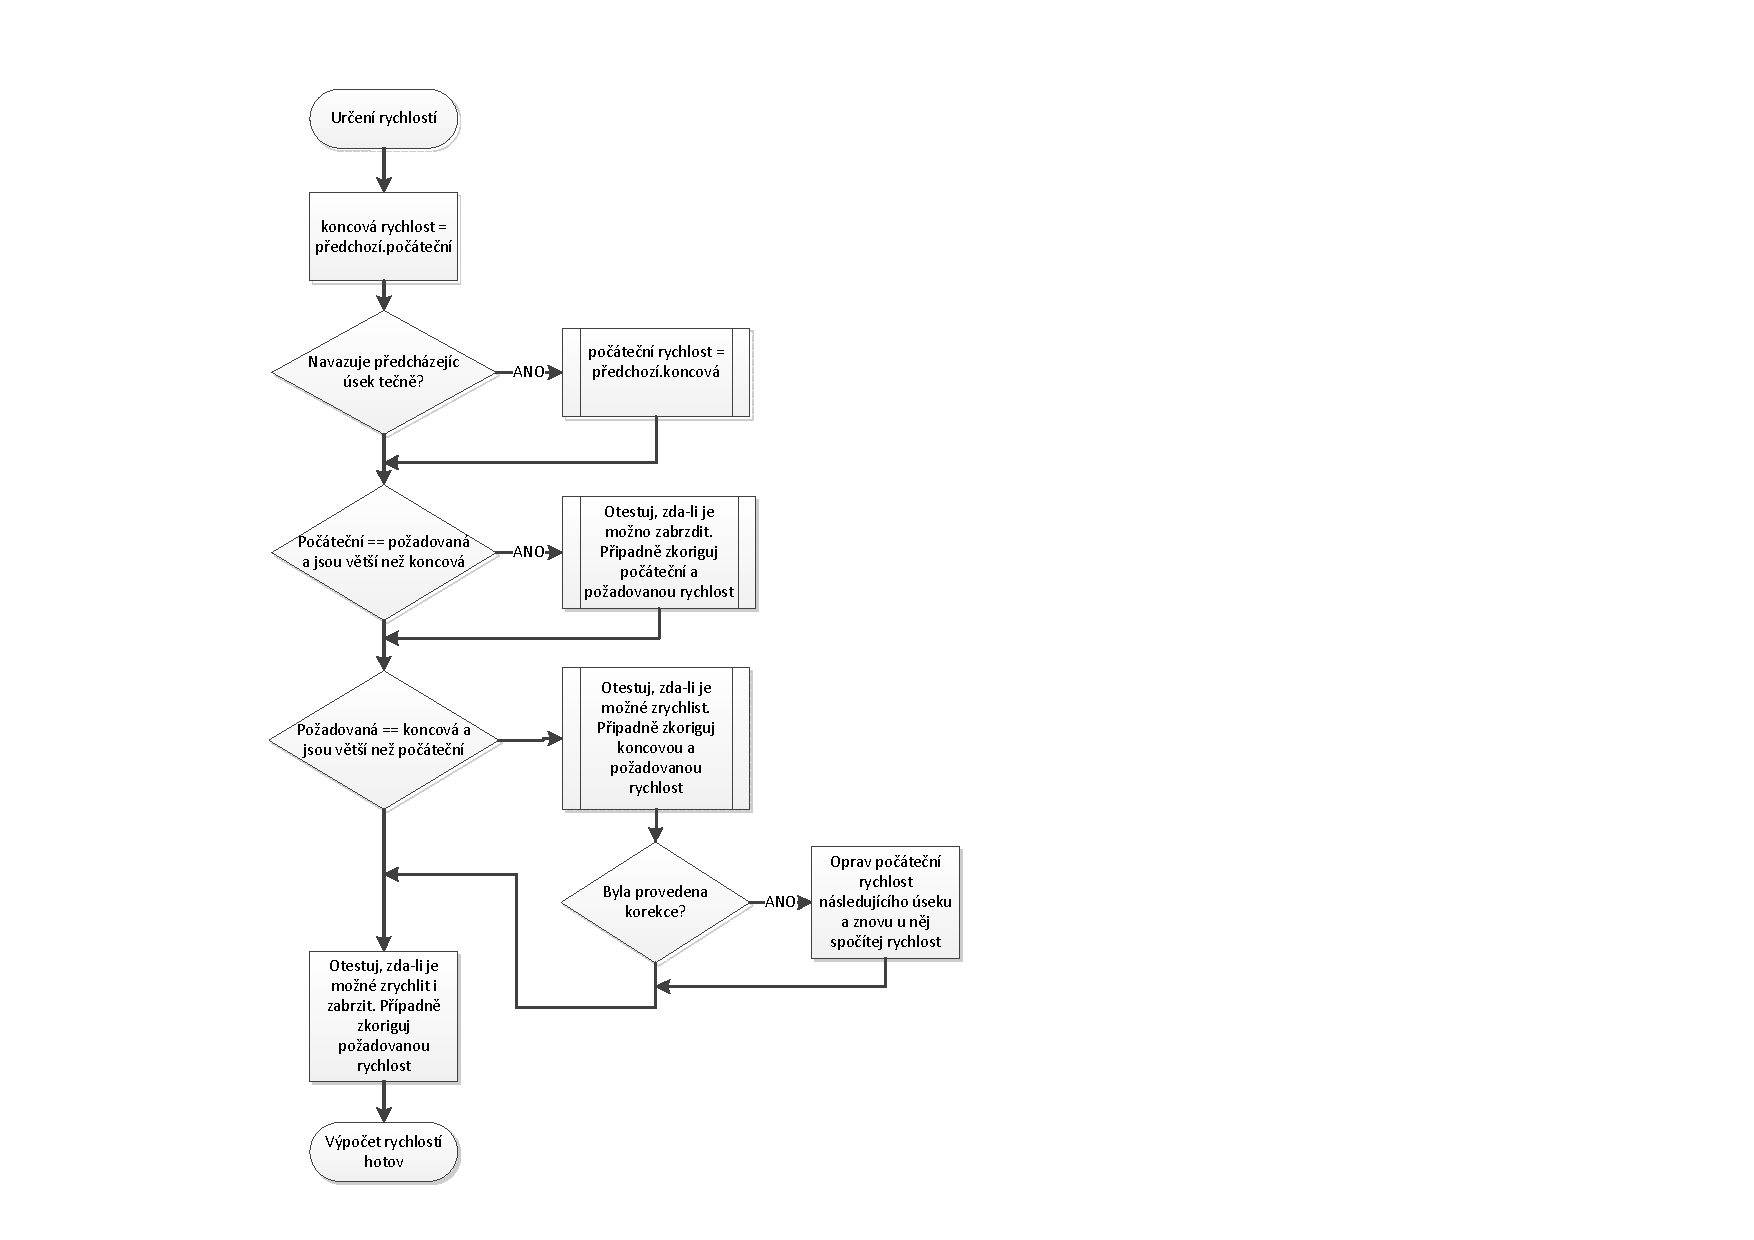
\includegraphics[width=0.7\textwidth]{img/vypocetrychlosti.pdf}
		\caption{Znázornění postupu výpočtu rychlosti daného úseku.}\label{nak:vypocet}	
	\end{figure}
	
	V každém úseku před zpracováním je počáteční a~koncová rychlost nastavena na nulu a~cílová rychlost je nastavena dle posuvu. Při výpočtu se koncová rychlost úseku nastaví na počáteční rychlost následujícího úseku. Poté se testuje, zda-li předcházející úsek navazuje tečně. Pokud ano, je současnému prvku nastavena počáteční rychlost rovna požadované rychlosti předchozího prvku (za podmínky, že je menší nebo rovna požadované rychlosti aktuálního prvku).
	
	Nyní je třeba otestovat, zda-li je možno požadovaných rychlostí dosáhnout na aktuálním úseku (jeho délce). Pro tento test je nutno spočítat rozjezdovou a~brzdnou dráhu (podrobněji popsáno v~kapitolách \ref{kap:drahlin} a~\ref{kap:rych-obl}).
	
	Test rychlosti probíhá v~několika úrovních. Pokud je počáteční rychlost rovna požadované a~zárověň jsou tyto rychlosti větší než koncová, je proveden test navíc - je totiž nutné určit, zda-li je možno na zadaném úseku ze zadané počáteční rychlosti zbrzdit na koncovou. Pokud ne, je nutné vhodně upravit počáteční (a požadovanou) rychlost.
	
	Následně se určí jak brzdná, tak rozjezdová dráha a~zkoumají se jejich hodnoty. Pokud je brzdná dráha nulová a~tedy požadovaná rychlost rovna koncové, zkoumá se, zda-li je možno požadované rychlosti dosáhnout. Pokud ne, je třeba snížit koncovou rychlost. Jelikož jsem změnil hodnotu koncové rychlosti, musím změnit hodnotu počáteční rychlosti následujícího úseku, který již byl zpracován, a~znovu jej zpracovat. Tento případ však nenastává často (to je důvod, proč zpracovávám úseky od~konce).
	
	Pokud brzdná dráha není nulová, nastává obecný případ. Pokud je součet obou drah větší než délka úseku, je nutné pomocí bisekce najít novou požadovanou rychlost. Tím je výpočet rychlosti na úseku vyřešen.
	
	\subsection{Určení rozjezdové a~brzdné dráhy při lineárním pohybu}\label{kap:drahlin}
	
	Určení délky rozjedové (brzné) dráhy při lineárním pohybu má na starosti metoda {\tt PathPartLine::GetSFromStartMovement}, resp. {\tt GetSFromEndMovement}. Tato metoda volá metodu {\tt PathPartLine::GetATFromMovement}, která na základě předané počáteční a~požadované rychlosti dopočte hodnoty maximální amplitudy zrychlení $A$ a~doby pohybu $T$ při zadaných omezeních. Poté z~těchto hodnot podle vztahu \ref{rov:lindrah} z~kapitoly \ref{kap:linrozbrzd} (resp. vztahu \ref{rov:lindrahb} pro brzdění) dopočte dráhu. Zároveň uloží vypočtené zrychlení do interního atributu {\tt Astart} (resp. {\tt Aend}) třídy {\tt PathPartMovable}, které je poté součástí příkazu pro interpolátor.
	
	Metoda {\tt GetATFromMovement} prvně testuje, zda-li nejsou předané rychlosti stejné. Pokud ano, vrátí nulový čas a~maximální možné zrychlení. Pokud ne, pokusí se prvně dopočítat čas pohybu za omezení ryvem. Využívá k~tomu vztah \ref{rov:linTJ}. Z~vypočteného času poté určí potřebnou amplitudu zrychlení. Pokud je tato amplituda menší než konfigurací nastavená maximální hodnota, vrátí funkce již vypočtený čas a~příslušné zrychlení. Pokud by při omezení ryvem bylo přesáhnuto maximální zrychlení, je dopočten čas pohybu za omezení zrychlením dle vztahu \ref{rov:lincas}. Poté je navrácen tento nově vypočtený čas a~maximální přípustná hodnota zrychlení.
	
	\subsection{Určení rozjezdové a~brzdné dráhy při pohybu po oblouku}\label{kap:rych-obl}
	I u obloukového pohybu jsou použity pro výpočet drah metody {\tt GetSFromStartMovement} a~{\tt GetSFromEndMovement}. Tyto metody volají přetíženou metodu {\tt GetATFromMovement}, která vrací příslušné hodnoty $A$ a~$T$ pro pohyb na oblouku pro předané rychlosti za daných omezení. Metoda {\tt GetSFromStartMovement} (resp. {\tt GetSFromEndMovement}) využívá pro určení dráhy stejné vztahy jako její obdoba pro lineární pohyb.
	
	Metoda {\tt GetATFromMovement} prvně zkontroluje, zdali je možno požadované rychlosti dosáhnout -- podmínka vyplývající ze~vztahu \ref{rov:oblpodm}. Tato podmínka je zde pro debuggovací účely -- již v dřívějších krocích by mělo být zajištěno, aby požadovaná rychlost nepřekračovala tuto mezní hodnotu.
	
	Funkce dále samostatně řeší případ, kdy je požadovaná rychlost rovna mezní hodnotě. V~tomto případě prvně počítám hodnoty $A$ a~$T$ za omezení ryvem s~jeho maximální hodnotou v~$t=0$, jelikož výpočet s~maximem v~$t=\frac{3T}{4}$ je výpočetně náročnější (je řešen numericky), proto jej počítám pouze v~krajním případě. K~výpočtu těchto hodnot jsou použity vztahy \ref{rov:linTJ} a~\ref{rov:oblA}. Na základě spočítaného $A$ a~$T$ dopočítám hodnotu ryvu v~čase $t=\frac{3T}{4}$ (dle prvního vztahu ze soustavy \ref{rov:oblJT}). Pokud je tato hodnota vyšší než hodnota v~čase $t=0$, musím omezit pohyb ryvem s~maximem v~$t=\frac{3T}{4}$. Tento numerický výpočet provádí metoda {\tt ComputeATLimitedByJerk} popsaná v~sekci \ref{kap:newton}. 
	
	Pokud požadovaná rychlost nedosahuje mezní hodnoty, jsou hodnoty $A$ a~$T$ určeny obdobně. Pouze je na závěr ještě nutno provést test, zda-li nebylo překročeno maximální zrychlení. Tento test není nutno v~mezním případě provádět, protože maximum zrychlení automaticky nastává v~čase $t=T$ a~dosahuje přesně mezní hodnoty. Maximum celkového zrychlení zde nastává v~čase $t=\frac{T}{2}$ a~pro jeho výpočet je použit vztah \ref{rov:oblak}. Pokud je překročeno, je nutné pohyb limitovat zrychlením. Příslušné hodnoty $A$ a~$T$ v~tomto případě určují vztahy \ref{rov:oblt2a}.
	
		\subsubsection{Řešení soustavy rovnic Newtonovou metodou}\label{kap:newton}
		Pro výpočet rychlosti, kdy maximum ryvu nastává v~čase $t=\frac{3T}{4}$, je třeba vyřešit soustavu rovnic \ref{rov:oblJT}. Tato soustava však není řešitelná obecně, je třeba využít numerické metody. K~jejímu řešení v~mé implementaci používám Newtonovu metodu, jelikož se snadno aplikuje na soustavu rovnic a~rychle konverguje\cite{wiki:newton}. Postup, jak řešit soustavu rovnic Newtonovou metodou jsem čerpal z~dokumentu~\cite{newton}.
		
		Princip řešení soustavy rovnic Newtonovou metodou spočívá v~převedení hledaného kořene na vektor a~nahrazení derivace příšlušné funkce maticí parciálních derivací daných funkcí\cite{newton}. Soustavu rovnic tedy musím převést na funkci\cite{newton} 
		\begin{equation}
			\vec{f(x)}=
			\begin{pmatrix}
				f_1(x_1, x_2,~\hdots~, x_n) \\
				f_2(x_1, x_2,~\hdots~, x_n) \\
				\vdots	\\
				f_n(x_1, x_2,~\hdots~, x_n)
			\end{pmatrix},
		\end{equation}
		jejíž derivací je matice parciálních derivací\cite{newton}
		\begin{equation}
			D\vec{f(x)}=
			\begin{pmatrix}
			\frac{\partial f_1}{\partial x_1}(x) & \frac{\partial f_1}{\partial x_2}(x) & \cdots & \frac{\partial f_1}{\partial x_n}(x)\\
			\frac{\partial f_2}{\partial x_1}(x) & \frac{\partial f_2}{\partial x_2}(x) & \cdots & \frac{\partial f_2}{\partial x_n}(x)\\
			\vdots & \vdots & \ddots & \vdots\\
			\frac{\partial f_n}{\partial x_1}(x) & \frac{\partial f_n}{\partial x_2}(x) & \cdots & \frac{\partial f_n}{\partial x_n}(x)\\
			\end{pmatrix}
		\end{equation}
		Mnou hledaným kořenem soustavy je vektor $\vec{p}$, pro nějž platí\cite{newton}
		\begin{equation}
				\vec{f(p)}=0
		\end{equation}
		Rekurzivní vztah pro kořen soustavy tedy potom vypadá následovně\cite{newton}:
		\begin{equation}
			\vec{p_{n+1}}=\vec{p_n}-\left(D\vec{f(p_n)}\right)^{-1}\vec{f(p_n)}
		\end{equation}
		
		Implementace mého konkrétního problému Newtonovou metodou není složitá, jelikož mám pouze soustavu dvou rovnic, tudíž pracuji s~dvojrozměrným vektorem a~maticí 2$\times$2.
		
		Tím se mi výrazně zjednodušuje hledání inverzní matice parciálních derivací. Pokud mám matici 2$\times$2
		\begin{equation}
			A=\begin{pmatrix}
				a & b \\
				c & d
			\end{pmatrix},
		\end{equation}
		tak její inverzní matici můžu vypočítat následovně\cite{inverze}:
		\begin{equation}
		A^{-1}=\frac{1}{\det A}\begin{pmatrix}
						d & -b \\
						-c & a
					\end{pmatrix}=\frac{1}{ad-bc}\begin{pmatrix}
											d & -b \\
											-c & a
										\end{pmatrix}
		\end{equation}
		
		Následné přepsání do kódu už je pouze rutinní záležitost. Díky jednoduchosti hledání inverzní matice není nutno použít speciální knihovnu pro práci s~maticemi a~celý problém lze naimplementovat s~použitím několika málo proměnných.
		
		Soustava \ref{rov:oblJT} reprezentuje v~kladných hodnotách (jiné nemají pro můj problém smysl) dvě křivky se dvěma průsečíky, jak lze vidět na grafu \ref{graf:newton}. Rovnice má tedy dva reálné kořeny v~kladných hodnotách (další reálné řešení se nachází v~záporném čase). První řešení s~nižší hodnotou času pohybu $T$, vždy přesahuje maximální zadanou hodnotu $A$ (experimentálně ověřeno na vzorku reálných dat). Za relevatní tedy považuji druhé řešení s~vyšší hodnotou periody $T$. Odtud se odvíjí můj odhad kořene pro Newtonovu metodu. Jako počáteční hodnotu volím dostatečně velkou hodnotu doby pohybu $T$ -- konkrétně stonásobek hodnoty vypočtené pomocí vztahu, který omezuje ryv v~čase $t=0$. Tím dosáhnu toho, že se k~hodnotě blížím zprava a~jako první naleznu pro mě relevantní řešení.
		
		\begin{figure}[h]
			\centering
			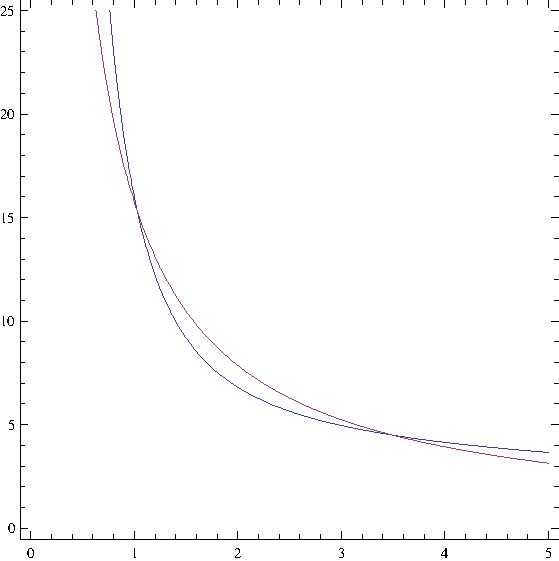
\includegraphics[width=0.5\textwidth]{img/graf_newton.pdf}
			\caption{Graf znázorňující řešení soustavy rovnic \ref{rov:oblJT}. Vodorovná osa reprezentuje dobu pohybu $T$, svislá amplitudu zrychlení $A$.}\label{graf:newton}	
		\end{figure}

		
	
	\subsection{Určení nové rychlosti pomocí bisekce}\label{kap:bisekce}
	
	Jak jsem zmínil v~předcházejícím textu, pro výpočet mezní rychlosti jsem použil metodu bisekce. Bisekce je též známá jako metoda půlení intervalů\cite{bisekce}. Tato metoda se zpravidla používá pro hledání kořene funkce mezi dvěmi zadanými mezemi. Metoda pracuje tak, že určuje, v~které polovině daného intervalu se nachází hledaná hodnota. Jakmile určí správný interval, rekurzivně se opakuje a~opět půlí tentokrát již menší interval\cite{bisekce}. Rekurze je ukončena, jakmile je buď nalezena správná hodnota, nebo je dosaženo požadované přesnosti.
	
	V praxi však není hojně používána, jelikož konverguje relativně pomalu (např. oproti Newtonově metodě). Avšak pro mě má bisekce výhodu v~tom, že ji lze použít nejen pro jednoduché hledání kořene, ale i k~hledání parametru v~určitém vztahu s~relativně složitou podmínkou, což je právě můj případ pro hledání rychlosti.
	
	Ačkoliv jsem v~kapitole \ref{kap:linryv} uvedl vztah, ze kterého lze Newtonovou metodou určit maximální dosažitelnou rychlost pro lineární pohyb, nepoužívám jej v~mém řídicím systému. Problémem tohoto řešení je, že je nutno vytvořit 4 varianty tohoto vztahu -- pro různé kombinace omezení rozjezdu a~brzdění omezeného ryvem či zrychlením. Také je nutné určit, který vztah je třeba použít. Výsledkem byl složitý kód, který měl podobnou časovou náročnost jako má současná implementace (avšak měl o něco lepší přesnost -- zde jsem generoval rychlost s~přesností 0,01~mm$\cdot$s$^{-1}$, nyní generuji rychlost s~přesností 0,1~mm$\cdot$s$^{-1}$, což je více než dostatečné). Situace pro výpočet rychlosti na oblouku byla ještě složitější a~počet variant zde prudce vzrostl. Proto jsem se rozhodl přiklonit k~metodě bisekce.
	
	Bisekci v~kódu implementuji pomocí cyklu. Tento cyklus probíhá, dokud velikost intervalu je větší než $0,1$ a~nebylo provedeno více než 10 iterací. V~tomto cyklu spočítám dráhu pro rychlost v~polovině daného intervalu. Na základě této dráhy a~podmínky rozhodnu, který interval budu dále půlit. Jako jedna hranice počátečního intervalu slouží nyní nevyhovující požadovaná rychlost a~jako druhá slouží počáteční nebo koncová rychlost -- podle toho, která z~nich je větší. Na reálných programech je rychlost s~přesností na 0,1~mm$\cdot$s$^{-1}$ dosažena během 4 iterací.
	
	\section{Komunikace s interpolátorem}
	
	Pro komunikaci s~interpolátorem přes USB používám knihovnu WinUSB. Tato knihovna obsahuje driver, který mi umožní z~user space operačního systému otevřít jednotlivé endpointy a~zapisovat na ně, popř. z~nich číst. Odprostí mě tak od~nutnosti psát vlastní driver v~kernel space\cite{winusb}.
	
	Ačkoliv je WinUSB dílem Microsoftu, musí tento ovladač projít stejným certifikačním procesem jako jakýkoliv jiný driver. To je pravděpodobně způsobeno tím, že pro použití musím upravit INF soubor ovladače, čímž poruším integritu dat a~již dříve udělený certifikát by se stal neplatným. Problematika ovladačů a~jejich certifikování na Windows je poměrně rozsáhlá a~bohužel se mi do ní nepodařilo zcela proniknout. Je možné, že mnou vytvořený certifikát a~vlastně i celý balíček ovladače nesplňuje všechny požadavky Microsoftu, avšak podařilo se mi jej nainstalovat na několika počítačích a~různých systémech (Windows XP, Windows 7 x86 i Windows 7 x64).
	
		\subsection{Tvorba balíčku ovladačů WinUSB}
		Aby WinUSB spolupracoval s~mým zařízením, je nutné upravit vzorový INF soubor\cite{winusb}. Tento soubor slouží jako popis driveru, resp. zařízení.
		
		V~sekci {\tt Version} je nutné vyplnit jméno poskytovatele driveru, uvést třídu zařízení, verzi a~datum vydání driveru, jeho GUID a~jako poslední také jméno souboru katologu. Katalog obsahuje hash všech souborů, které ovladač obsahuje a~tím slouží k~ověření, zda-li soubory nebyly modifikovány. K~ověření pravosti katalogu slouží certifikát, jak zmiňuji níže.
		
		GUID (Globally unique identifier) je 128 bitové číslo\cite{wiki:guid}. Toto číslo slouží jako identifikátor COM objektu, na základě něhož si je možné z~mé aplikace tento objekt vyvolat a~skrz něj komunikovat se zařízením. GUID se generuje náhodně -- vzhledem k~velikosti čísla je šance, že by se podařilo vygenerovat dvě stejná GUID velmi malá\cite{winusb}.
		
		V~sekci {\tt Manufacturer} je třeba nastavit identifikátor, resp. cestu k zařízení, pro jednotlivé platformy. Tato cesta je ve tvaru {\tt USB\textbackslash VID\_xxxx\&PID\_yyyy}, kde xxxx je příslušné vendor ID zařízení a~yyyy je příslušné product ID zařízení.
		
		Úpravou sekce {\tt SourceDisksNames} je možné docílit vlastního pojmenování instalačních disků (toto jméno se zobrazuje během instalace ovladače). Poslední sekcí, kterou je třeba upravit, je sekce {\tt Strings}. Touto sekcí lze nastavit jméno zařízení tak, jak se bude zobrazovat ve správci zařízení a~specifikovat výrobce, kterého lze zobrazit ve vlastnostech daného zařízení.
		
		Jakmile je INF soubor upraven, je třeba vytvořit katalog ovladače\cite{kernel}. Katalog zajišťuje integritu celého ovladače a~umožňuje systému před instalací ověřit, zda-li nebyl driver modifikován. Microsoft poskytuje utilitu zvanou Inf2Cat\cite{kernel}, která na základě předaného INF souboru vytvoří katalog všech souborů, na které INF soubor odkazuje. V~případě problémů je možné také použít utilitu MakeCat\cite{kernel}, která vytvoří katalog na základě předaného seznamu souborů.
		
		Následně je nutno katalog podepsat\footnote{Windows XP podepsání nevyžadují, avšak zobrazí varování o nedůvěryhodném driveru. Windows Vista a~výše však již podepsání vyžadují, jinak odmítnou ovladač nainstalovat.}, čímž je zajištěna jeho pravost. Toto podepsání lze provést pomocí utility SingTool\cite{kernel}. Pro podepsání je však třeba mít certifikát. Aby driver při instalaci do systému prošel bez chyby ověřovacím procesem, je třeba mít certifikát vydaný institucí schválenou Microsoftem\cite{kernel}. Tato možnost je relativně drahá a~hlavně pro fyzickou osobu nedostupná. Naštěstí Microsoft umožňuje pro vývojové účely vygenerovat si vlastní certifikát, který umožní katalog podepsat\cite{kernel}. Avšak při instalaci ovladače se zobrazí, že certifikát pochází od~nedůvěryhodné osoby. Tento certifikát je možné vygenerovat si pomocí utility MakeCert\cite{kernel}.
		
		Mnou upravený balíček ovladačů WinUSB, společně s~katalogem a~příslušnými utilitami lze nalézt na přiloženém CD.
		
		\subsection{Třída MyDevice}
		
		Třída {\tt MyDevice} reprezentuje rozhraní pro komunikaci s~interpolátorem. Zaobaluje veškerou funkcionalitu okolo WinUSB -- stará se o inicializaci zařízení (otevření endpointů), jeho správnou deinicializaci při ukončení aplikace a~reaguje na jeho připojení čí odpojení.
		
		Posílání zpráv do interpolátoru je realizováno metodou {\tt SendRawData}, která přebírá data k odeslání buď jako ukazatel na pole a~jeho délku nebo jako {\tt std::vector<char>}. Tato metoda zkontroluje, zda-li je zařízení připojeno a~případně odešle data do interpolátoru pomocí funkce {\tt WinUsb\_WritePipe} přes příslušný endpoint. Jelikož je obrovské množství zpráv, které je možné do zařízení odeslat, nedefinuje tato třída pro každou zprávu speciální metodu, ale raději poskytuje obecnou metodu pro zápis libovolných dat. V~mém návrhu existuje pouze několik málo speciálních zpráv (požadavků, na které je očekávána odpověď), pro které je definována speciální metoda. Tyto požadavky jsou popsány v~následujícím odstavci.
		
		Třída {\tt MyDevice} také uchovává objekt třídy {\tt ReceiveFromDevice}, který se stará o příchozí data. Tato třída je popsána v~následující podkapitole. Ve spolupráci s~ní definuje třída {\tt MyDevice} speciální metody {\tt GetFreeSpaceInQueue}, {\tt GetLastProcessedItemStack}, {\tt GetCurrentlyProcessed-ItemStack}. Tyto metody odešlou příslušnou zprávu pro intepolátor (dle svého názvu) a~čekají na odpověď. Jsou tedy definovány jako blokující (proto by neměly být volány ve vláknu uživatelského rozhraní). Jako návratovou hodnotu mají již zpracovanou odpověď na danou zprávu.
		
		\subsection{Třída ReceiveFromDevice}
		
		Třída {\tt ReceiveFromDevice} je potomkem třídy {\tt wxThread} -- reprezentuje tedy vlákno. Uvnitř tohoto vlákna je v~nekonečném cyklu volána blokující funkce {\tt WinUsb\_ReadPipe}, která čte z~daného endpointu. Tato třída skládá dohromady zprávy rozdělené na více paketů stejně jako to dělá interpolátor (popsáno v~kapitole \ref{kap:protokol}). Pro každou přijatou zprávu pak volá metodu {\tt ProcessMessage}. V~této metodě je definováno zpracování všech možných zpráv.
		
		\subsection{Třídy ProgramControl a~ProgramRun}
		
		Nejdůležitějším typem komunikace je odesílání příkazů interpolátoru do jeho komponenty {\tt CommandStack}, odkud jsou postupně vykonávány. Další důležitou funkcí je zpětná vazba o poloze stroje, která je následně zobrazována uživateli. Tyto operace má na starosti třída {\tt ProgramRun}, která je ovládána třídou {\tt ProgramControl}.
		
		Třída {\tt ProgramRun} je potomkem třídy {\tt wxThread} -- reprezentuje tedy vlákno. Proto jsem pro interakci tohoto vlákna se zbytkem aplikace implementoval třídu {\tt ProgramControl}. Třída {\tt ProgramControl} při spuštění vykonávání programu v~G-kódu vytvoří novou instanci třídy {\tt ProgramRun}. Tuto třídu, respektive vlákno, poté ovládá pomocí příznaků. Příznak může mít tři stavy -- stav signalizující běžící program, stav signalizující pozastavení vykonávání a~stav zastavení programu.
		
		Během běhu programu třída {\tt ProgramRun} se neustále dotazuje interpolátoru na volné místo v~zásobníku a~pokud nějaké volné místo je, odešle patřičný počet příkazů do interpolátoru. Zároveň také posílá dotaz na aktuální pozici stroje. Tento dotaz je posílán v~neblokujícím režimu, jelikož jeho výsledek není nutný pro další běh vlákna (na~rozdíl od~dotazu na volné místo). Odpověď na pozici stroje zpracuje třída ReceiveFromDevice, která zajistí předání dat na správné místo tak, aby byla pozice stroje uživateli znázorněna.
		
		Pokud je běh programu pozastaven, pošle vlákno interpolátoru příkaz pro zastavení aktuálně vykonávané činnosti a~čeká na znovuobnovení běhu programu.
		
		Pokud je program zastaven, odešle vlákno interpolátoru příkaz pro zastavení aktuálně vykonávané činnosti a~příkaz pro vyprázdnění zásobníku příkazů. Poté se vlákno ukončí.